\documentclass{report}

\usepackage{fullpage}
\usepackage{physics}
\usepackage{hepnicenames}
\usepackage{booktabs}
\usepackage{siunitx}
\usepackage{hyperref}
\usepackage{feynmp-auto}
\usepackage{pdfpages}
\usepackage{bm}
\usepackage{mathtools}
\usepackage{subcaption}

\setlength{\parindent}{0pt}
\setlength{\parskip}{1em}

% Bold vectors
\renewcommand{\vec}[1]{\bm{\mathrm{#1}}}
% Trace operator
\DeclareMathOperator{\tr}{Tr}
% Feynman slash
\newcommand{\fsl}[1]{\ensuremath{\mathrlap{\!\not{\phantom{#1}}}#1}}


\begin{document}

  \begin{titlepage}
    \phantom{\,}
    \vfill
    \centering
    {\huge\textbf{The Standard Model}}\\
    \vspace{\parskip}
    {\Large\textbf{Part I}}
    \vspace{5em}
    \vfill
  \end{titlepage}

  \chapter*{Acknowledgements}
These notes were orignially made during a course of lectures delivered as part of an intercollegiate postgraduate course in high-energy physics at the University of London from September to December 2015.

They are based on lectures by Dr Mario Campanelli (UCL) and previous notes written by Sam Cook and Aidan Randle-Conde.

Some textbooks were also used for reference. These include:
\begin{itemize}
  \item F. Halzen, and A.D. Martin. \textsl{Quark & Leptons: An Introductory Course In Modern Particle Physics.} John Wiley & Sons, 2008.
  \item M. Peskin, and D. Schroeder. \textsl{An introduction to quantum field theory.} 1995.
  \item J. Binney, and D. Skinner. \textsl{The physics of quantum mechanics.} Oxford University Press, 2013.
  \item M. Thomson. \textsl{Modern particle physics.} Cambridge University Press, 2013.
\end{itemize}


  \tableofcontents

  \chapter{Introduction: Matter and Forces}
The definition of the Standard Model (SM) is not fully agreed upon in the scientific community. The minimal acceptable definition is that of the unified electroweak (EW) interaction according to Glashow, Salam, and Weinberg (GSW). Quantum chromodynamics (QCD) explains the strong force, but there is currently no theory of unified EW and QCD interactions. The most commonly used Standard Model is that of EW plus QCD interactions. In this model, neutrinos are massless. However, in principle, the SM could include the phenomena of neutrino oscillations by adding a kinetic term to the Standard Model Lagrangian, $\mathcal{L}_{SM}$. If neutrinos were found to be Majorana fermions (their own antiparticles), this would explain the small neutrino mass. The widest definition of the Standard Model includes general relativity and cosmology. This extreme version is not generally used, since its large- and small-scale behaviours cannot presently be unified. In what follows, we work with SM = EW + QCD.

\section{Matter content of the universe}
The Standard Model splits the fundamental particles into fermions (spin-$\frac{1}{2}$) and bosons (integer spin). Fermions are the building-blocks of matter due to the Pauli exclusion principle. The fundamental bosons are the results of gauge invariances and serve to mediate the forces of the Standard Model.

Fermions are further divided into leptons and quarks.

\subsection{Leptons}
\begin{table}[h]
\centering
\begin{tabular}{cccc}
\toprule
I & II & III\\
\midrule
$\begin{pmatrix}\Pnue \\ \Pe \end{pmatrix}$ &
$\begin{pmatrix}\Pnum \\ \Pmu \end{pmatrix}$ &
$\begin{pmatrix}\Pnut \\ \Ptau \end{pmatrix}$ \\
\bottomrule
\end{tabular}
\caption{The leptons of the Standard Model arranged into three generations. The top row has charge $Q=0$ and the bottom row $Q=-1$.\label{tab:leptons}}
\end{table}

\begin{table}
\centering
\begin{tabular}{cc}
\toprule
\Plepton & Mass \\
\midrule
\Pe & \SI{511}{\kilo\electronvolt\per c^2} \\
\Pmu & \SI{106}{\mega\electronvolt\per c^2} \\
\Ptau & \SI{1.78}{\giga\electronvolt\per c^2}\\
\bottomrule
\end{tabular}
\caption{The masses of the charged leptons.\label{tab:leptonMass}}
\end{table}

Leptons do not experience the strong force (they are color neutral) and do not mix. Due to its mass, the \Ptau lepton can decay hadronically, whereas muon decay is purely leptonic. The most common muon decay is \HepProcess{\Pmuon\to\Pelectron\Pnum\APnue}.

\subsection{Quarks}
Similarly, the three generations of quarks are organised into isospin doublets.
\begin{table}[h]
\centering
\begin{tabular}{ccc}
\toprule
I & II & II \\
\midrule
$\begin{pmatrix}\Pup \\ \Pdown \end{pmatrix}$ &
$\begin{pmatrix}\Pcharm \\ \Pstrange \end{pmatrix}$ &
$\begin{pmatrix}\Ptop \\ \Pbottom \end{pmatrix}$ \\
\bottomrule
\end{tabular}
\caption{The quarks arranged into three isospin doublets. The top row has its third component of isospin $I_3=+\frac{1}{2}$ and the bottom $I_3=-\frac{1}{2}$. Equivalently, they have charges $Q=+\frac{2}{3}$ and $Q=-\frac{1}{3}$, respectively.\label{tab:quarks}}
\end{table}

It is difficult to assign masses to the individual quarks since they are always bound. Most of the proton's mass is created dynamically by the strong interaction between the light valence quarks. For heavy quarks, assigning a mass from the difference between hadron masses becomes easier, and approximate masses are given in Table \ref{tab:quarkMass}.

\begin{table}[h]
\centering
\begin{tabular}{cc}
\toprule
\Pquark & Mass \\
\midrule
u & \SI{2.2}{\mega\electronvolt\per c^2}\\
d & \SI{5}{\mega\electronvolt\per c^2}\\
c & \SI{1.25}{\giga\electronvolt\per c^2}\\
s & \SI{95}{\mega\electronvolt\per c^2}\\
t & \SI{174.2}{\giga\electronvolt\per c^2}\\
b & \SI{4.2}{\giga\electronvolt\per c^2}\\
\bottomrule
\end{tabular}

\caption{Approximate quark masses. It is difficult to assign masses to the lighter quarks due to quark confinement and their strong interactions (see main body).\label{tab:quarkMass}}.
\end{table}

\subsection{Bosons}
The fundamental Standard Model bosons and their properties are listed in Table \ref{tab:boson}.
\begin{table}[h]
\centering
\begin{tabular}{ccccc}
\toprule
& Spin & Charge & Mass & Force \\
\midrule
\Pphoton & 1 & 0 & 0 & EM \\
\PWpm & 1 & $\pm1$ & \SI{80.4}{\giga\electronvolt\per c^2} & Weak \\
\PZ & 1 & 0 & \SI{91.2}{\giga\electronvolt\per c^2} & Weak \\
\Pgluon & 1 & 0 & 0 & Strong\\
\PHiggs & 0 & 0 & \SI{125}{\giga\electronvolt\per c^2} & - \\
\bottomrule
\end{tabular}
\caption{The fundamental bosons of the Standard Model. The Higgs boson, \PHiggs, does not mediate a force but rather is required for the \PW and \PZ bosons to have mass under electroweak symmetry breaking.\label{tab:boson}}
\end{table}

Quarks may combine to form hadrons that are non-fundamental bosons, e.g.~$J^P(\Ppiplus)=0^-$.

\section{Forces}
At our energy scale there are four fundamental forces of nature: electromagnetism (EM), weak, strong, and gravity.

Gravity does not currently have a quantum formulation. Quantum gravity (QG) is in its theoretical infancy and, as shown below, experiments cannot reach the energy scales required for gravity to manifest itself at subatomic scales.

\subsection{Gravity}
Our best understanding of gravity -- that of general relativity (GR) -- describes the force as a result of the geometrical properties of spacetime. As such, GR predicts the existence of gravitational waves; ripples in spacetime emerging from extreme astrophysical situations causing large masses to oscillate. Gravitational waves have not yet been directly observed, but observations from Hulse and Taylor over a 17 year period observed a change in the period of a binary neutron star system. This change can only be accounted for by gravitational radiation, thus the experiment is an indirect detection of gravitational waves. This work won the Nobel Prize in 1993.

Gravity is known to be by far the weakest of the four fundamental forces. It is thought to be mediated by a spin-2 boson, the graviton. The strength of a force is proportional to the exchange momentum of the mediating boson, so very large energies will be required to observe gravity in a collider.

For a theory of everything (TOE), there is some energy scale at which gravity will unify with the Standard Model describing EW and QCD interactions. This is called the Planck mass and is derived here from the uncertainty principle.

\subsubsection{The Planck mass}
According to the uncertainty principle, a particle with mass $m$ can exist for time
\begin{equation}
\delta t \sim \frac{\hbar}{mc^2}
\end{equation}
with a characteristic range
\begin{equation}
\delta r = \delta t \times c = \frac{\hbar}{mc}.
\end{equation}
At this separation from the point mass, the gravitational potential energy between two particles with mass $m$ is
\begin{equation}
V = \frac{Gm^2}{\delta r} = \frac{Gm^3c}{\hbar}.
\end{equation}
When this potential energy is similar to a particle's mass energy, then gravitational effects become important and a theory of quantum gravity is needed. This occurs when $V \sim mc^2$, i.e.~
\begin{equation}
\frac{Gm^3c}{\hbar} \sim mc^2
\end{equation}
which is rearranged to define the Planck mass
\begin{equation}\boxed{
m_\text{Planck} \equiv \sqrt{\frac{\hbar c}{G}}
}
\end{equation}
whose value is of the order \SI[retain-unity-mantissa = false]{1e19}{\giga\electronvolt\per c^2}. Similarly, we may define the Planck length $\lambda_\text{Planck} \sim \SI[retain-unity-mantissa = false]{1e-35}{\meter}$, and the Planck time $t_\text{Planck} \sim \SI[retain-unity-mantissa = false]{1e-43}{\second}$.

When calculating integrals in the Standard Model (such as when evaluating loops in Feynman diagrams), the upper limit of integration should be the Planck scale, since this is where our understanding of nature breaks down.

\subsubsection{Dark matter}
Dark matter is believed to constitute about 25\% of the matter-energy content of the universe. This comes from observations of the rotational velocity curve of galaxies.

A simple model of a galaxy has a uniformly distributed spherical core with mass density $\rho$ at radii below $R$ and zero above. At gravitational equilibrium inside the galaxy, the centripetal force on some test star with mass $m$ is equal to the gravitational pull from the core inside the shell at distance $r$ from the centre,
\begin{align}
\frac{mv^2}{r} &= \frac{GmM(r)}{r^2} \\
\Rightarrow \quad v^2 &= \frac{GM(r)}{r} \\
&= \frac{GM_\text{galaxy}}{r}\left(\frac{r}{R}\right)^3\\
\Rightarrow \quad v &= \sqrt{\frac{GM_\text{galaxy}}{R^3}} \, r.
\end{align}
Outside the galaxy core we expect
\begin{equation}
v = \sqrt{\frac{GM_\text{galaxy}}{r}}.
\end{equation}
The observed discrepancy is known as the galaxy rotation problem, where the mass distribution of the galaxy is calculated from its luminous regions. The solution to the problem predicts a halo of dark matter around the edge of the galaxy.

Candidates for dark matter include:
\begin{itemize}
\item Massive cool hadronic objects (MaCHOs). Brown dwarves are small, dark stars that have been observed via gravitational lensing. A large abundance of MaCHOs is unlikely due to the known baryonic makeup of the early universe. There is not a sufficient number of MaCHOs to account for the dark matter problem.
\item Neutrinos. Since the mass of the neutrino is almost zero, neutrinos form hot dark matter. They carry thermal energy away from hot areas of the universe and do not cluster as halos around galaxies.
\item Supersymmetric particles as cold dark matter. Cold dark matter (CDM) must be made up of heavy particles for little thermal movement. Supersymmetric particles are the favourite CDM candidates in light of observations such as the anisotropy of the early universe. Supersymmetry (SUSY) solves some problems of the Standard Model and provides a natural CDM candidate, a particle with mass $\sim \SI{100}{\giga\electronvolt/c^2}$. These heavy particles are known as WIMPs (weakly interacting massive particles).
\item Light supersymmetric particles (LSPs) or hidden sector. Not yet explored area of particle physics could yield CDM candidates. There could be less massive particles that interact very weakly with ordinary matter; this is called the hidden sector. Additional theories of supersymmetry could predict light weakly interacting particles.
\end{itemize}

\subsection{Electromagnetism}
The electromagnetic (EM) force is described in the Standard Model by quantum electrodynamics (QED). All EM interactions involve the exchange of a virtual photon. The strength of the electromagnetic interaction is given by\begin{equation}
\frac{e^2}{q^2}
\end{equation}
where $q$ is the virtual photon's 4-momentum. $e$ is the electromagnetic coupling constant and is related to the fine structure constant by
\begin{equation}
e = \sqrt{4\pi\alpha}.
\end{equation}
The fine structure constant is itself defined as the ratio of the energy to overcome electrostatic repulsion between two electrons a distance $r$ apart and the energy of a photon of wavelength $\lambda = 2\pi r$.,
\begin{equation}
\alpha = \frac{e^2}{4\pi \epsilon_0 r} \left/ \frac{hc}{\lambda} \right. = \frac{e^2}{4\pi \epsilon_0 r} \left/ \frac{\hbar c}{r} \right. = \frac{e^2}{4\pi \epsilon_0 r \hbar c}.
\end{equation}
In natural units, where $\hbar = c = \epsilon_0 = 1$, this becomes
\begin{equation}
\boxed{\alpha = \frac{e^2}{4\pi}}.\label{eq:fineStructure}
\end{equation}


\subsection{The weak force}
The Fermi theory of weak interactions treats the nuclear beta decay as a single four-point vertex with strength $g_F$. The reaction is
\begin{equation}
\HepProcess{\Pneutron \to \Pproton + \Pelectron + \APnue}.
\end{equation}
A more sophisticated treatment recognises the role of the virtual W boson being exchanges as quarks change flavor,
\begin{equation}
\HepProcess{\Pdown \to \Pup + \PWminus \to \Pup + \Pelectron + \APnue}.
\end{equation}

In contrast to the EM interaction above, the strength of an interaction involving the exchange of the massive \PW boson is
\begin{equation}
\frac{g_W^2}{q^2 + m_W^2}
\end{equation}
where $g_W$ is similar to the electromagnetic $e$. This means, at energies much less than the \PW mass, $q^2 \ll m_W^2$, the weak force is much weaker than the electromagnetic force. However, for energies near to and above the \PW mass, $q^2 \geq m_W^2$, the forces are comparable and unify at energies around \SI{100}{\giga\electronvolt} or greater.

To first order, individual lepton numbers (i.e.~electron, muon, tau number) are conserved in weak interactions. This is equivalent to saying there is no mixing in the lepton sector, since leptons do not experience the strong force. Some example weak processes follow.
\begin{align}
\HepProcess{\Pnue + \Pneutron \to \Pproton + \Pelectron} \\
\HepProcess{\APnue + \Pproton \to \Pneutron + \Ppositron} \\
\HepProcess{\Pmuon \to \Pelectron + \Pnum + \APnue}
\end{align}

\subsection{The strong force}
Protons and neutrons are confined to the nucleus, so there must be a force which overcomes the electrostatic repulsion of the positive EM charges and also acts on neutrons. In scattering experiments,
\begin{equation}
\Ppiplus + \Pproton \xrightarrow{\Delta^{++}(1238)} \Ppiplus + \Pproton
\end{equation}
a resonance peak was seen at \SI{1238}{\mega\electronvolt\per c^2}, corresponding to the $\Delta^{++}$ resonance with valence quark contents $\Pup\Pup\Pup$. Since all three quarks in the baryon have the same spatial wavefunction, flavor, and at least two must have the same spin projection, this violates the exclusion principle without further quantum numbers. Introducing a color quantum number, with three color charges, solves this problem and provides a mechanism responsible for nuclear structure and quark confinement. The extra quantum number also means that for every hadronic decay there are three possible final states, giving a three-times color degeneracy to those decay modes.

The $SU(3)$ gauge model of the strong force results in an octet of gluons, which can self-interact via three- and four-point vertices. These extra vertices mean there are many more QCD diagrams for a given process, and calculating amplitudes in QCD is, in general, quite difficult. Furthermore, the QCD coupling constant is large -- owing to its high strength versus the electromagnetic interaction -- so, in general, one cannot stop with the first-order diagram. However, the running of the strong coupling constant means it decreases at high energies, so at LHC energies it is possible to use perturbation theory with QCD processes.

\section{Local gauge invariance}
The Lagrangian of a gauge theory is invariant under local transformations belonging to a particular symmetry group. This gauge invariance gives rise to the forces in the Standard Model -- EW and QCD. Why nature insists on gauge invariance is unknown.

As an example, consider a scalar theory of electromagnetism. Local gauge invariance under transformations belonging to the group $U(1)$ requires the Lagrangian is invariant to a rotation in phase space,
\begin{equation}
\psi(x, t) \rightarrow e^{i\alpha(x)} \psi(x, t).
\end{equation}
The transformation is said to be \emph{local} becuase the phase $\alpha(x)$ is a general function of space. Now requiring $\delta\mathcal{L}=0$ leads to the introduction of a massless gauge field, $A^\mu$; this is the photon field.

Similarly, local gauge invariance under transformations belonging to the groups $SU(2)$ and $SU(3)$ gives rise to the weak and strong forces, respectively. In this approach, however, the gauge bosons are all required to be massless, contrary to observations.

\section{Spontaneous symmetry breaking}

The EM and weak interactions have been successfully unified. That is, they have been shown to be two manifestations of the same [$SU(2) \times U(1)$] electroweak (EW) force, which they become at a higher energy (around \SI{100}{\giga\electronvolt}\footnote{In fact, the phase transition occurs at the Higgs vacuum expectation value (VEV), about \SI{246}{\giga\electronvolt}. The strength of the EM and weak forces merge at around \SI{100}{\giga\electronvolt}, so they appear as similar forces.}). As the universe cooled below this electroweak unification energy, the distinct EM and weak forces we see at normal energies froze out of the more general EW force. The spontaneous symmetry breaking leading to the EM and weak forces was described by Glashow, Salam, and Weinberg (GSW). The mechanism that allows the \PW and \PZ bosons to have mass after the EW symmetry breaking is the Higgs mechanism, of which the Higgs boson is a result. The strong force is described by quantum electrodynamics (QCD) and has not yet been unified with the EW interaction.

\section{Grand unified theories}

A grand unified theory (GUT) would bring the EW and QCD interactions together under a grand unified group, $G$ or $SU(5)$. Such theories would have to restore the broken symmetry we observe between colorless leptons and colored quarks, allowing quarks to turn into antileptons and vice versa. These interactions would violate conservation of baryon number, $B$, but $B-L$ (where $L$ is lepton number) would be conserved. The exchange boson is called the $X$ boson, which would have a mass of order \SI[retain-unity-mantissa = false]{1e6}{\giga\electronvolt\per c^2} and hence a range $10^{-4}$ times the weak force's.

This GUT force hence predicts the decay of the proton, which has not yet been observed although current experiments are attempting to measure the lifetime of the proton, if it is indeed unstable. An example decay is \HepProcess{\Pproton \to \Ppositron + \Ppizero}.

  \chapter{Experimental Concepts}
This chapter serves as a reminder of commonly used ideas in high-energy physics (HEP) experiments.

\section{Experimental possibilities}
In reality there are rather few experimental possibilities for HEP experiments:
\begin{itemize}
\item Scatter one particle off another and observe the reaction;
\item Generate a particle in a reaction and observe its decay;
\item Detect neutrinos and observe neutrino oscillations;
\item Measure a particular particle's properties such as mass, charge, spin, parity, lifetime.
\end{itemize}

\section{Cross section}
The cross section, $\sigma$, for a particular reaction is proportional to the probability for the interaction to take place. In HEP experiments, it is expressed in the unit barns, where $\SI{1}{\barn} = \SI{1e-28}{\meter^2}$.

\subsection{Beam incident on a target}
Assume the beam is comprised of bunches with $N_B$ particles per bunch. The beam is incident on a target with area $A$, length $l$ inside the luminous region, and mass density $\rho$. Then the number of target particles seen by the beam is
\begin{equation}
N_T = \frac{Al\rho N_A}{m}
\end{equation}
where $N_A$ is Avagadro's number and $m$ is the molecular mass, such that $N_A/m$ is the mass of each target particle.

Now we can define the cross section as
\begin{align}
P(\text{interaction}) &= (\text{Number of target particles per unit area}) \times \sigma \\
&= \frac{Al\rho N_A}{m} \times \frac{\sigma}{A} \nonumber \\
&= \frac{l\rho N_A \sigma}{m}.
\end{align}
Therefore the total number of interactions per bunch is given by
\begin{equation}
N_I = \frac{l\rho N_A N_B \sigma}{m}.
\end{equation}
Now take the target and bunch to contain number densities $n_B$ and $n_T$ of particles, respectively. They have relative speed $u \simeq c$. Then the number of target particles in the luminous region is $n_T V$, so the probability of interaction may now be written
\begin{equation}
P(\text{interaction}) = \frac{n_T V \sigma}{A}.
\end{equation}
There are $n_B u A$ beam particles passing through the luminous region per second, so the rate of interactions is
\begin{equation}
\frac{\dd N_I}{\dd t} = n_B n_T V u \sigma.
\end{equation}

\subsection{Beam-beam collision}
For a circular collider, assume a rotation frequency $f$ for both counter-circulating beams consisting of $n$ bunches, each with $N_B$ particles and area $A$. Then the rate of interactions is
\begin{align}
\frac{\dd N_I}{\dd t} &= P(\text{collision}) \times (\text{particles per second in one beam}) \\
&= \frac{N_B \sigma}{A} \times n f N_B \nonumber \\
&= \frac{n f N_B^2 \sigma}{A} \label{eq:collRate}.
\end{align}

\section{Luminosity}
Using the result from \eqref{eq:collRate}, we define the instantaneous luminosity
\begin{equation}\boxed{
L \equiv \frac{1}{\sigma} \frac{\dd N_I}{\dd t}
}\end{equation}
hence for beam-beam collisions
\begin{equation}
L = \frac{n f N_B^2}{A}.
\end{equation}

In an effort to increase the luminosity, focussing magnets near to the collision regions are used to decrease the bunch area. Also, the number of particles per bunch should be made as large as possible while also maintaining a stable bunch.

Spontaneous luminosity tends to decrease with run time due to collision remnants decreasing the vacuum in the beam pipe and consequently deforming the bunches. An LHC beam has a typical lifetime of around 10--15 hours (the lifetime is the time for $L$ to decay by a factor $e$). At this point the beam is dumped and a new beam is accelerated and injected into the storage ring ready for collisions.

The units of $L$ are typically \si{\per \pico\barn \per \second}. To get a measure of the total number of interactions observed, and hence the amount of data collected, $L$ may be integrated to give the integrated luminosity,
\begin{equation}\boxed{
L_\text{int} = \int L \, \dd t
}
\end{equation}
which often has the units of inverse femtobarns, \si{\per \femto \barn}.

\section{Natural units and conversion factors}
In natural units, we have $\hbar = c = 1$. $c$ is the conversion factor between space and time or mass and energy, and $\hbar$ is the conversion between energy and time. Consider the units of their product:
\begin{align}
[\hbar c] &= [ET][LT^{-1}] \nonumber \\
&= [E][L].
\end{align}
Now we have $c = \SI{3e8}{\meter\per\second}$ and $\hbar = \SI{1.05e-34}{\joule\second} = \SI{6.56e-22}{\mega\electronvolt\second}$, so
\begin{equation}\boxed{
\hbar c = \SI{197}{\mega \electronvolt \femto \meter} \equiv 1}.
\end{equation}
Therefore, we have
\begin{equation}
\SI{1}{\giga\electronvolt} = \frac{1000}{\SI{197}{\femto\meter}} = \SI{5.08e15}{\per\meter} = \SI{1.52e24}{\per\second}
\end{equation}
\begin{equation}
\Rightarrow\quad \frac{1}{\si{\giga\electronvolt^2}} = \SI{3.88e-32}{\meter^2} = \SI{0.388}{\milli\barn}.
\end{equation}

  \chapter{Experiments of the Last 60 Years}

  \chapter{Non-Relativistic Quantum Mechanics}
Here an overview of some basic results from Schr{\"o}dinger and Heisenberg's quantum mechanics are given. The quantum harmonic oscillator (QHO) is solved exactly, and extended to the anharmonic case with first-order perturbation theory. Lagrangian mechanics is briefly covered, before some consideration of the important Dirac $\delta$ and Heaviside $\theta$ step functions.

A time-varying quantum state my be expressed by a vector $\ket{\psi(t)}$. In the position representation, this yields the wavefunction, $\psi(x, t) \equiv \braket{x}{\psi(t)}$.

\section{Schr{\"o}dinger's equation and probability current density}
We start from the classical energy-momentum relation for a non-relativistic particle with mass $m$,
\begin{equation}
E = \frac{p^2}{2m}. \label{eq:energyMomentum}
\end{equation}
Replace the energy with the operator $E\rightarrow\hat{E} = i \frac{\partial}{\partial t}$ and momentum with $p\rightarrow \hat{p} = -i \vec{\nabla}$. Then \eqref{eq:energyMomentum} becomes the time-dependent Schr dinger equation (TDSE),
\begin{equation}
i \frac{\partial \psi}{\partial t} = -\frac{1}{2m} \nabla^2 \psi \label{eq:schrodinger}.
\end{equation}
Multiplying this by the complex conjugate of the wavefunction, $\psi^*$,
\begin{equation}
i \psi^* \frac{\partial \psi}{\partial t} = -\frac{1}{2m} \psi^* \nabla^2 \psi \label{eq:part1}.
\end{equation}
Take the complex conjugate of \eqref{eq:schrodinger} and multiply by $\psi$,
\begin{equation}
-i \frac{\partial \psi^*}{\partial t} \psi = -\frac{1}{2m} (\nabla^2 \psi^*) \psi \label{eq:part2}.
\end{equation}
Subtracting \eqref{eq:part2} from \eqref{eq:part1},
\begin{equation}
i\left( \psi^*\frac{\partial \psi}{\partial t} + \frac{\partial \psi^*}{\partial t} \psi \right) = -\frac{1}{2m} \left[ \psi^* (\nabla^2 \psi) - \psi (\nabla^2 \psi^*) \right]
\end{equation}
and rearranging using the product rule,
\begin{equation}
\frac{\partial}{\partial t}(\psi^*\psi) + \frac{i}{2m} \vec{\nabla}\cdot \left[ \psi(\vec{\nabla}\psi^*) - (\vec{\nabla}\psi)\psi^* \right] = 0.
\end{equation}
This is nothing but a continuity equation for the probability density $\rho = \psi^*\psi = \abs{\psi}^2$ and the probability current density $\vec{j} = \frac{i}{2m}\left[ \psi(\vec{\nabla}\psi^*) - (\vec{\nabla}\psi)\psi^* \right]$.

\subsubsection{Application to a plane wave}
Consider a free plane wave whose wavefunction is given by $\psi(x, t) = \mathcal{N} e^{i(\vec{p}\cdot\vec{x} - Et)}$, where $\mathcal{N}$ is a normalisation constant. Then, applying the definitions for $\rho$ and $\vec{j}$ above,
\begin{align}
\rho &= \abs{\psi}^2 = \abs{N}^2 \\
\vec{j} &= \frac{i}{2m}\left[ \psi(\vec{\nabla}\psi^*) - (\vec{\nabla}\psi)\psi^* \right] = \frac{\abs{N}^2}{m} \vec{p}
\end{align}

\section{Heisenberg and interaction pictures}\
\subsection{Heisenberg picture}
In the above, we have used the Schr{\"o}dinger picture where operators remain constant in time, and the states can vary. In contrast, the Heisenberg picture treats the states as constants, and the operators evolve in time. To show that these are equivalent, solve the time-independent Schr{\"o}dinger equation for an energy eigenstate $\ket{\psi(t)}$.
\begin{align}
i \frac{\dd \ket{\psi(t)}}{\dd t} &= \hat{H} \ket{\psi(t)} \\
\Rightarrow\quad \int\limits_0^t \frac{\dd \ket{\psi(t^\prime)}}{\ket{\psi(t^\prime)}} &= -i \int\limits_0^t \hat{H} \, \dd t^\prime \\
\Rightarrow\quad \ket{\psi(t)} &= e^{-i\hat{H}t} \ket{\psi(0)} \quad \text{for time-independent $\hat{H}$.} \label{eq:evolution}
\end{align}
In quantum mechanics, observables connect the theory with measurements. Observable quantities are expectation values of operators. Consider some general operator, $\hat{A}$, whose expectation value is given by
\begin{align}
\expval{A} &= \expval{\hat{A}}{\psi(t)} \\
&= \expval{e^{i\hat{H}t}\hat{A}e^{-i\hat{H}t}}{\psi(0)}.
\end{align}
Therefore, it is equivalent to define time-independent states and time-dependent operators in the Heisenberg picture:
\begin{align}
\ket{\psi_H} &\equiv \ket{\psi(0)} \\
\hat{A}_H &\equiv e^{i\hat{H}t}\hat{A}e^{-i\hat{H}t}.
\end{align}
Then the expectation value is simply
\begin{equation}
\expval{A} = \expval{\hat{A}_H}{\psi_H}
\end{equation}
and
\begin{align}
\dv{\hat{A}_H}{t} &= i\hat{H}e^{i\hat{H}t}\hat{A}e^{-i\hat{H}t} - ie^{i\hat{H}t}\hat{A}\hat{H}e^{-i\hat{H}t} \nonumber \\
&= i(\hat{H}\hat{A} - \hat{A}\hat{H}) \nonumber \\
&= i [ \hat{H}, \hat{A} ]
\end{align}

\subsection{The interaction picture}
In the interaction picture, both states and operators have some time dependance. In the interaction picture, we split the Hamiltonian into a free part $\hat{H}_0$ and interaction part $\hat{H}^\prime$,
\begin{equation}
\hat{H} = \hat{H}_0 + \hat{H}^\prime.
\end{equation}
The free part is generally time-independent and easily solved. We then say that operators $\hat{A}_I$ evolve according to the free part of the Hamiltonian,
\begin{equation}
\hat{A}_I(t) = e^{i\hat{H}_0t}\hat{A}e^{-i\hat{H}_0t}.
\end{equation}
Then the operator in the interaction picture evolves according to
\begin{equation}
\dv{\hat{A}_I}{t} = i [ \hat{H}_0, \hat{A}_I(t) ].
\end{equation}
Now consider the expectation value of the operator, $\expval{A} = \expval{e^{i\hat{H}_0t}\hat{A}e^{-i\hat{H}_0t}}{\psi_I(t)}$. We see that for this to be equivalent to the Schr{\"o}dinger picture expectation value, the states must evolve according to the interaction part of the Hamiltonian $\hat{H}^\prime$,
\begin{equation}
\ket{\psi_I(t)} = e^{-i\hat{H}^\prime t}\ket{\psi(0)}
\end{equation}
or equivalently
\begin{equation}
\ket{\psi_I(t)} = e^{i\hat{H}_0 t}\ket{\psi(t)}.
\end{equation}
The interaction picture is used in the perturbative expansion of the $S$-matrix in quantum field theory (QFT). This leads to the concept of using Feynman diagrams to calculate amplitudes.

Note that the three different pictures of quantum mechanics coincide at $t=0$.

\section{Quantum harmonic oscillator}
The quantum harmonic oscillator is an exactly solvable problem that neatly introduces ladder operators.

Consider a Hamiltonian of the form
\begin{equation}
H = \frac{p^2}{2m} + \frac{1}{2} m \omega^2 x^2
\end{equation}
where it should be clear from the context which quantities are operators, so we drop the hat notation, $\hat{O} \rightarrow O$.

Introduce the ladder operator
\begin{equation}
a = \frac{m \omega x + ip}{\sqrt{2m\omega}}
\end{equation}
and bearing in mind that $x$ and $p$ are hermitian,
\begin{equation}
a^\dagger = \frac{m \omega x - ip}{\sqrt{2m\omega}}.
\end{equation}
The product $a^\dagger a$ is
\begin{align}
a^\dagger a &= \frac{(m \omega x - ip)(m \omega x + ip)}{2 m \omega} \nonumber \\
&= \frac{1}{2m\omega} \left\{ (m \omega x)^2 + im\omega [x, p] + p^2 \right\} \nonumber \\
&= \frac{H}{\omega} - \frac{1}{2}.
\end{align}
Rearranging, the Hamiltonian can be written
\begin{equation}
H = \left( a^\dagger a + \frac{1}{2} \right) \omega.
\end{equation}
Similarly,
\begin{equation}
a a^\dagger = \frac{H}{\omega} + \frac{1}{2}.
\end{equation}
We also have that
\begin{equation}
[a, a^\dagger] = 1
\end{equation}
and
\begin{align}
[a, H] &= \omega a\\
[a^\dagger, H] &= -\omega a^\dagger.
\end{align}

\subsection{Energy spectrum}

Now consider the action of the operator $a^\dagger$ on a stationary state $\ket{n}$ with some energy $E_n$. What is the energy of the state $A^\dagger \ket{n}$?
\begin{align}
H a^\dagger \ket{n} &= \left( a^\dagger H - [a^\dagger, H] \right)\ket{n} \nonumber \\
&= \left( a^\dagger H + \omega a^\dagger \right)\ket{n} \nonumber \\
&= \left( E_n + \omega \right) a^\dagger \ket{n}.
\end{align}
So $a^\dagger\ket{n}$ is also an energy eigenstate with energy $\left( E_n + \omega \right)$. Since $a^\dagger$ has raised the energy of the state $\ket{n}$ by one quantum of energy, we call it the raising operator.

Similarly, the application of $a$ to $\ket{n}$ lowers the energy by $\omega$,
\begin{equation}
H a \ket{n} = (E_n - \omega) a \ket{n}.
\end{equation}
$a$ is called the lowering operator and together $a$ and $a^\dagger$ are ladder operators that span the energy spectrum of the QHO. In QFT, these operators correspond to the creation and annihilation of particles since particles are wave excitations of the vacuum.

\subsection{Zero-point energy}
There must be some state $\ket{0}$ for which $a\ket{0}$ vanishes. Equating to zero the square length of this state vector,
\begin{align}
0 = \abs{a\ket{0}}^2 &= \expval{a^\dagger a}{0} \\
&= \expval{\frac{H}{\omega} - \frac{1}{2}}{0} \nonumber \\
&= \frac{E_0}{\omega} - \frac{1}{2}.
\end{align}
Rearranging gives the energy of the vacuum state, $\ket{0}$,
\begin{equation}
E_0 = \frac{\omega}{2}.
\end{equation}

\subsection{Action of the ladder operators}

Now we can build up the ladder of energy states by continuous action of the raising operator,
\begin{align*}
a^\dagger\ket{0} &= \alpha_0 \ket{1} \\
a^\dagger\ket{1} &= \alpha_1 \ket{2} \\
\ldots \\
a^\dagger\ket{n} &= \alpha_n \ket{n+1}
\end{align*}
where the normalisation constant can be found via
\begin{align}
\alpha_n^2 = \abs{a^\dagger\ket{n}} &= \expval{a a^\dagger}{n} \nonumber \\
&= \expval{\frac{H}{\omega} + \frac{1}{2}}{n} \nonumber \\
&= n+1
\end{align}
so $\alpha_n = \sqrt{n+1}$. Therefore the general action of the raising operator is
\begin{equation}
\boxed{
a^\dagger \ket{n} = \sqrt{n+1}\ket{n+1}
}.
\end{equation}
Similarly,
\begin{equation}
\boxed{a \ket{n} = \sqrt{n} \ket{n-1}}.
\end{equation}

A general state $\ket{n}$ can be made from repeated application of $a^\dagger$ from the ground state:
\begin{equation}
\ket{n} = \frac{1}{\sqrt{n!}} (a^\dagger)^n \ket{0}.
\end{equation}


Notice that $a^\dagger a \ket{n} = n \ket{n}$, so $a^\dagger a$ is called the number operator.

\section{The anharmonic oscillator (perturbation theory)}
We now generalise the above QHO to include an anharmonic term,
\begin{align}
H &= \frac{p^2}{2m} + \frac{1}{2}m \omega^2 x^2 + \lambda x^3 \\
&= H_0 + \lambda H^\prime
\end{align}
where the second line expresses the Hamiltonian as in the interaction picture. In this case, the interaction hamiltonian is $H^\prime = x^3$. In what follows, we assume that $\lambda$ is small such that $H^\prime$ is a perturbation to the QHO solution and we stop expansions after first order in $\lambda$.

The eigenvectors of the full Hamiltonian may be expanded as
\begin{equation}
\ket{n} = \ket{n}^0 + \lambda\ket{n}^1 + \cdots
\end{equation}
where all the $\ket{n}^i$ are assumed to be orthogonal. The state has corresponding energy
\begin{equation}
E_n = E_n^0 + E_n^1 + \ldots
\end{equation}
such that it is the solution of the TISE,
\begin{align}
H\ket{n} &= E_n\ket{n} \\
\left( H_0 + \lambda H^\prime + \ldots \right)\left( \ket{n}^0 + \lambda\ket{n}^1 + \ldots \right) &= \left( E_n^0 + \lambda E_n^1 + \ldots \right)\left( \ket{n}^0 + \lambda\ket{n}^1 + \ldots \right)
\end{align}

Equating the coefficients of $\lambda^0$ gives the trivial harmonic part of the solution,
\begin{equation}
H_0 \ket{n}^0 = E_n^0 \ket{n}^0.
\end{equation}
Equating the coefficients of $\lambda^1$ gives
\begin{equation}
H_0\ket{n}^1 + H^\prime\ket{n}^0 = E_n^0\ket{n}^1 + E_n^1\ket{n}^0. \label{eq:lambda1}
\end{equation}
Rearranging and multiplying by $^0\!\bra{n}$,
\begin{equation}
^0\!\bra{n}H_0 - E_n^0\ket{n}^1 + ^0\!\bra{n}H^\prime - E_n^1\ket{n}^0 = 0.
\end{equation}
Now use that $^0\!\bra{n}H_0 = \,^0\!\bra{n} E_n^0$ to see that the first term is equal to zero. This gives the solution for the change in energy (up to first order in $\lambda$) of the $n$th excited state,
\begin{equation}\boxed{
E_n^1 = \,^0\!\expval{H^\prime}{n}^0
}.
\end{equation}

Now we wish to find the first-order correction to the state, $\ket{n}^1$. First, use the representation of $\ket{n}^1$ in the basis of harmonic solutions, $\ket{m}^0$,
\begin{equation}
\ket{n}^1 = \sum_m \ket{m}^0 \, ^0\!\braket{m}{n}^1 \label{eq:spectrum}.
\end{equation}
The eigenstates of the harmonic problem $\ket{m}^0$ may serve as a basis since they are all orthonormal, i.e.~$^0\!\braket{m}{n}^0 = \delta_{nm}$.

Now to get the coefficients $^0\!\braket{m}{n}^1$, multiply \eqref{eq:lambda1} by $^0\!\bra{m}$,
\begin{equation}
\underbrace{^0\!\bra{m}H_0\ket{n}^1}_{E_m^0 \,^0\!\braket{m}{n}^1} + ^0\!\bra{m}H^\prime\ket{n}^0 = ^0\!\bra{m}E_n^0\ket{n}^1 + \underbrace{^0\!\bra{m}E_n^1\ket{n}^0}_0.
\end{equation}
Rearranging,
\begin{equation}
^0\!\braket{m}{n}^0 = \frac{^0\!\bra{m}H^\prime\ket{n}^0}{E_n^0 - E_m^0} \label{eq:coefficients}.
\end{equation}
Notice that this approach only works if the energy levels are non-degenrate, i.e.~$E_n^0 \neq E_m^0$ for all $n \neq m$. For the QHO this is the case, but in more general cases one must diagonalise the Hamiltonian first.

Now, substituting \eqref{eq:coefficients} into \eqref{eq:spectrum} gives the value of the first-order correction to the energy eigenstates,
\begin{equation}
\boxed{
\ket{n}^1 = \sum_m \frac{^0\!\bra{m}H^\prime\ket{n}^0}{E_n^0 - E_m^0} \ket{m}^0
}.
\end{equation}

In the particular case where $H^\prime = x^3$ it is helpful to express the perturbation in terms of the ladder operators,
\begin{equation}
x^3 = \frac{(a + a^\dagger)^3}{(2m\omega)^\frac{2}{3}}.
\end{equation}
Then the determination of $E_n^1$ and $\ket{n}^1$ is achievable via the application of the ladder operators to the QHO eigenstates.

\section{Lagrangian mechanics}
In general, a Lagrangian is a function of coordinates $q$ and their derivatives, $L = L(q, \dot{q})$. The action is the integral of $L$,
\begin{equation}
S = \int L(q, \dot{q}) \, \dd t.
\end{equation}
Classical paths are those paths with stationary action, where $\delta S = 0$. This requires,
\begin{align}
\delta S &= \int \dd t \left\{ \pdv{L}{q} \delta q + \pdv{L}{\dot{q}} \delta\dot{q} \right\} \\
&= \int \dd t \left\{ \left[ \pdv{L}{q} - \dv{t}\left( \pdv{L}{\dot{q}} \right) \right] \delta q \right\} + \left[ \pdv{L}{\dot{q}} \delta q \right]_{t_1}^{t_2} = 0.
\end{align}
The last term is a total derivative and vanishes for any $\delta q$ that decays at spatial infinity and obeys $\delta q(t_1) = \delta q(t_2)$. For all such paths, we obtain the Euler-Lagrange equations of motion,
\begin{equation}
\boxed{
\pdv{L}{q} - \dv{t} \left( \pdv{L}{(\dot{q})} \right) = 0
}.
\end{equation}

\subsection{Relation to the Hamiltonian}

Each coordinate $q$ has a conjugate momentum,
\begin{equation}
p = \pdv{L}{\dot{q}}.
\end{equation}
Then the Hamiltonian is related to the Lagrangian by
\begin{equation}
\boxed{
H = p\dot{q} - L
}
\end{equation}

For a quantum treatment, we replace the coordinates with operators. The operators and their conjugate momenta have the commutation relations
\begin{equation}
[\hat{q}, \hat{p}] = i
\end{equation}
in natural units.

\subsection{Application to the QHO}
The QHO Lagrangian is
\begin{equation}
L = \frac{1}{2}m\dot{x}^2 - \frac{1}{2}m\omega^2 x^2.
\end{equation}
Therefore the momentum, $p = \pdv{L}{\dot{x}} = m\dot{x}$. So the Hamiltonian is
\begin{align}
H &= p\dot{x} - L \\
&= \frac{p^2}{m} - \left(\frac{1}{2}m\dot{x}^2 - \frac{1}{2}m\omega^2 x^2\right)\\
&= \frac{1}{2}m\dot{x}^2 + \frac{1}{2}m\omega^2 x^2
\end{align}
which is the same as we used for the QHO above.

The Lagrangian and Hamiltonian treatments are equivalent, but often a problem is more soluble in one over the other. QFT makes use of the Lagrangian density, and this is used to express the particles and interactions of the Standard Model.

\section{Dirac $\delta$ function}
The $\delta$ function may be thought of as a peaked function of width $\Delta x$ and height $1/\Delta x$ around a value $x=x_0$ in the limit $Delta x \rightarrow 0$. It has the properties
\begin{equation}
\int\limits_{-\infty}^{+\infty} \delta(x - x_0) \, \dd{x} = 1
\end{equation}
and
\begin{equation}
\int\limits_{-\infty}^{+\infty} f(x) \, \delta(x - x_0) \, \dd{x} = f(x_0).
\end{equation}
As a result, $\delta(x) - \delta(-x)$ is an even function and $\delta{ax} = \delta{x}/\abs{a}$. The proof is as follows:
\begin{align}
\int\limits_{-\infty}^{+\infty} \delta(ax) \, \dd{x} &= \int\limits_{-\infty}^{+\infty} \delta(y) \, \frac{\dd{y}}{a} \quad \text{for $y=ax$,} \\
&= \frac{1}{\abs{a}}.
\end{align}
Now consider a function $f(x)$ with roots $a_i$ such that $f(a_i)=0$. Then $\delta(f(x))$ function is non-zero only in the vicinity $x \sim a_i$. Expanding $f(x)$ about a particular root,
\begin{equation}
f(x) = \underbrace{f(a_i)}_0 + (x-a_i)\left[ \pdv{f}{x} \right]_{x=a_i} + \ldots
\end{equation}
so, using the preceding result, we have
\begin{align}
\delta(f(x)) &= \sum_i \delta\left((x-a_i)\left[\pdv{f}{x}\right]_{x=a_i}\right)\\
&= \sum_i \frac{\delta(x-a_i)}{\left|\pdv{f}{x}\right|_{x=a_i}}.
\end{align}


The $\delta$ function is normally constructed by taking the limit of some test function. Here, various test functions are discussed.

\subsubsection{Discrete $\delta$ function}
Consider some function $f(x)$ as a set of values $x_i$ in bins of width $\Delta x$. Then the integral becomes a discrete sum,
\begin{equation}
\int\limits_{-\infty}^{+\infty} f(x) \, \delta_t(x - x_0) \, \dd{x} \rightarrow \sum_{i={-\infty}}^{+\infty} f(x_i) \, \delta(x_i-x_0) \Delta x
\end{equation}
where $\delta_t(x - x_0) = 0$ for $i \neq 0$ and $\delta_t(0) = 1/\Delta{x}$. In the limit $\Delta x \rightarrow 0$, $\delta_t$ becomes the Dirac $\delta$ function. However, it is not particularly useful to have a discrete, non-differentiable definition.

\subsubsection{Breit-Wigner lineshape}
Consider a test function of a Breit-Wigner resonance peak,
\begin{equation}
\delta_t(x) = \frac{1}{\pi} \frac{\epsilon}{x^2 + \epsilon^2}.
\end{equation}
Its integral is
\begin{equation}
\int\limits_{-\infty}{+\infty} \frac{1}{\pi} \frac{\epsilon}{x^2 + \epsilon^2} \, \dd{x} = \int\limits_{-{\pi}/{2}}^{+{\pi}/{2}} \frac{1}{\pi} \frac{\sec^2{\theta}}{1+\tan^2{\theta}} \, \dd{\theta} = 1
\end{equation}
where the substitution $x = \epsilon \tan \theta$ has been used. At $x=0$, $\delta_t(0) = 1/\pi\epsilon$ and the full width at half-maximum is $2\epsilon$. The Breit-Wigner lineshape approaches the Dirac $\delta$ function in the limit $\epsilon\rightarrow 0$.

\subsubsection{Fourier analysis}
The Fourier integral theorem states that
\begin{equation}
f(x) = \frac{1}{2\pi} \int\limits_{-\infty}^{+\infty} e^{ipx} \left( \int\limits_{-\infty}^{+\infty} e^{-p\alpha} f(\alpha) \, \dd{\alpha} \right) \, \dd{p}.
\end{equation}
That is, the reverse transform of the Fourier transform of a function returns the original function. Rearranging\footnote{Cauchy showed that the order of integration matters, but this rearrangement is justified under the \emph{theory of distributions}.},
\begin{equation}
f(x) = \frac{1}{2\pi} \int\limits_{-\infty}^{+\infty} \left( \int\limits_{-\infty}^{+\infty} e^{pix} e^{-ip\alpha} \, \dd{p} \right) f(\alpha) \, \dd{\alpha} = \int\limits_{-\infty}^{+\infty} \delta(x-\alpha) f(\alpha) \, \dd{\alpha}
\end{equation}
where we see the $\delta$ function can now be defined
\begin{equation}
\delta(x) = \frac{1}{2\pi} \int\limits_{-\infty}^{+\infty} e^{ipx} \, \dd{p}.
\end{equation}

\section{Heaviside step function}
The Heaviside step function is defined in discrete form
\begin{equation}
\theta(x) =
\begin{cases}
1 & x > 0 \\
0 & x < 0
\end{cases}
\end{equation}

An integral representation for $\theta$ can be reached through recognising that its derivative is the Dirac $\delta$ function,
\begin{equation}
\dv{\theta}{x} = \delta(x) = \frac{1}{2\pi} \int\limits_{-\infty}^{+\infty} e^{ipx} \, \dd{p}.
\end{equation}
Integrating with respect to $x$,\begin{align}
\theta(x) &= \frac{1}{2\pi} \int\limits_{-\infty}^{+\infty} \int e^{ipx} \, \dd{p} \, \dd{x} \\
&= \frac{1}{2\pi i} \int\limits_{-\infty}^{+\infty} \frac{e^{ipx}}{p} \dd{p}
\end{align}
where the constant of integration is zero. Adding a small offset to the denominator, we get the final integral form of the $\theta$ step function
\begin{align}
\theta(x) = \lim_{\epsilon\rightarrow 0^+} \frac{1}{2\pi i} \oint_C \frac{e^{ipx}}{p+i\epsilon} \, \dd{p}.
\end{align}
where $C$ is a contour along the real axis closed in the upper-half plane.

The residue theorem states that
\begin{equation}
\oint_C \frac{f(z)}{z-a} \dd{z} = 2\pi i f(a)
\end{equation}
for a contour $C$ containing $a$. Applying this to the integral representation for $\theta$ above,
\begin{equation}
\theta(x) = \lim_{\epsilon\rightarrow 0^+} \frac{2\pi i}{2\pi i} e^{ip(-i\epsilon)} = \lim_{\epsilon\rightarrow 0^+} e^{p\epsilon} = 1
\end{equation}
for $x > 0$. For $x < 0$, the contour must be closed in the lower-half plane and the integral evaluates to $0$.

  \chapter{Special relativity}
The study of high energy physics involves particles travelling at speeds close to $c$ and often with energies much greater than their mass. Therefore, much of the notation and calculations used stem from a proper treatment of special relativity (SR).

\section{4-vectors}
SR places space and time on an equal footing and they adopt the same units in the system of natural units. We combine the information in time and space as components in a 4-vector, for example,
\begin{align*}
x^\mu = \mqty(t \\ \vec{r}), \quad p^\mu = \mqty(E \\ \vec{p}).
\end{align*}
Note that in contravariant form (with the index up), 4-vectors are written as column vectors.

The metric tensor is a symmetric matrix that tells us how to link space and time. In the case of special relativity, it is simply a diagonal matrix\footnote{The $(+,-,-,-)$ signature is most often used in high energy physics since most 4-vector quantities we deal with will be timelike. By contrast, general relativity usually uses the $(-,+,+,+)$ signature. Using either signature is valid, but it is important to not confuse them.},
\begin{equation}
g_{\mu\nu} = \mqty(\dmat{1,-1,-1,-1}) = g^{\mu\nu}.
\end{equation}
The metric tensor may be used to perform index gymnastics to raise or lower an index. For example, we can find the covariant forms of the above 4-vectors,
\begin{align*}
x_{\mu} = g_{\mu\nu}x^\nu = (t,\, -\vec{r}), \quad p_{\mu} = g_{\mu\nu}p^\nu = (E,\, -\vec{p}).
\end{align*}

The scalar product of two 4-vectors is given by
\begin{equation}
a_{\mu} b^{\mu} = g_{\mu\nu}a^{\nu}b^{\mu} = b_{\mu} a^{\mu}.
\end{equation}

Note the scalar product is invariant to which vector is covariant. Often, when only dealing with scalar products, we use the notation of a capital letter with no index for a 4-vector: $X$, $P$, $A$, etc. Then a scalar product may be written, for instance, as $XX = X^2$.

Finally, introduce the 4-vector derivative in covariant form,
\begin{equation}
\partial_\mu = \left( \pdv{t},\, \vec{\nabla} \right).
\end{equation}
then its square length is
\begin{equation}
\partial^2 = \partial_\mu \partial^\nu = \left(\pdv{t}\right)^2 - \nabla^2.\label{eq:nablaSquared}
\end{equation}

\section{Lorentz transformation}
The Lorentz transformation is given by $x^\mu \rightarrow (x^\prime)^\mu$ where
\begin{equation}
\mqty(t^\prime \\ x^\prime \\ y^\prime \\ z^\prime) = \mqty(\dmat{\gamma&{-\beta\gamma}\\{-\beta\gamma}&\gamma, 1, 1}) \mqty(t\\ x\\ y\\ z)
\end{equation}
for a 4-vector boosted by speed $\beta$ along the $x$-axis. For completeness, we define $\gamma$ here,
\begin{equation}
\gamma = \frac{1}{\sqrt{1-\beta^2}}.
\end{equation}

The scalar product $a_\mu b^\mu$, and in fact any fully-contracted quantity, is invariant under Lorentz transformations, since they do not depend on the coordinates.

\section{The light cone}
Consider two events with 4-coordinates $X$ and $Y$. The square of their spacetime separation is given by
\begin{equation}
s^2 = (X-Y)^2 = (t_x - t_y)^2 - (\vec{x} - \vec{y})^2.
\end{equation}
Along the surface of the light cone, $s=0$. This condition gives
\begin{equation}
t_x - t_y = \abs{\vec{x} - \vec{y}}
\end{equation}
i.e.~if a flash of light is emitted at $X$, it reaches $\vec{y}$ at $t_y$. If $s^2 > 0$, then $t_x - t_y > \abs{\vec{x} - \vec{y}}$ and a light pulse emitted at $X$ reaches $\vec{y}$ before $t_y$. Therefore, the events are causally connected and their separation is said to be timelike. For $s^2<0$, the events are have spacelike separation and are causally disjoint.

\section{Relativistic kinematics}
In particle physics, there are two processes we could consider. Firstly, the decay of one particle into daughter particles,
\begin{equation}
A \to B + C + \ldots
\end{equation}
where the simplest case is that of two-body decay, \HepProcess{A\to B+C}. Here the centre of mass (CM) energy is simply the mass of the parent particle, $m_A$. Secondly, a scattering process,
\begin{equation}
A + B \to C + D + \ldots
\end{equation}
where the CM energy is given by $E_{CM}^2 = (P_A + P_B)^2 = (P_C + P_D + \ldots) ^2$ (recall that $P_i$ is a 4-momentum).

\subsection{Fixed target particle production}
Consider the process
\begin{equation}
A + B \to C
\end{equation}
where the target $B$ is at rest in the laboratory frame. Therefore, $P_B = (m_B, \vec{0})$.

The centre of mass energy is given by
\begin{align}
E_{CM}^2 &= (P_A + P_B)^2 \\
&= E_A^2 + 2E_A m_B + m_B^2 - \abs{\vec{p_A}}^2
\end{align}
Use that $E_A^2 - \abs{\vec{p_A}}^2 = m_A^2$,
\begin{equation}
E_{CM}^2 = m_A^2 + m_B^2 + 2E_A m_V
\end{equation}
A typical beam has energy much greater than either of the masses involved, so we may write
\begin{equation}
\boxed{
E_{CM} \approx \sqrt{2 E_A m_B}
}
\end{equation}

At the production threshold, $E_{CM} = E_C$. This means that for a proton target ($m_B \sim \SI{1}{\giga\electronvolt}$), the incident particle energy required to produce a Higgs boson ($m_C \sim \SI{100}{\giga\electronvolt}$) is about \SI{5}{\tera\electronvolt}. For a hadronic beam about one tenth of the beam energy goes into collisions so this would require a \SI{50}{\tera\electronvolt} beam. In fact, fixed-target collisions rarely even produce \Pbottom quarks. This means fixed-target experiemnts are not suitable for modern high-energy discoveries with present accelerator technology, and we must instead look towards beam-beam colliders.

\subsection{Beam-beam collisions}
In this type of collider, two beams are collided with opposite momenta:
\begin{align*}
P_A = \mqty(E_A \\ \vec{p}), \quad P_B = \mqty(E_B \\ -\vec{p})
\end{align*}
so the CM frame is the laboratory frame:
\begin{equation}
P_{CM} = P_A + P_B = \mqty(E_{CM} \\ \vec{0}) = \mqty(E_A + E_B \\ \vec{0}).
\end{equation}
We want to find the required energy for one of the beams, $E_A$, as a function of $E_{CM}$. Start by considering the product
\begin{align}
P_A P_{CM} &= \left( E_A,\, \vec{p} \right) \mqty(E_{CM} \\ \vec{0}) = E_A E_{CM} \\
\text{also,}\quad P_A P_{CM} &= P_A (P_A + P_B) = P_A^2 + P_A P_B \label{eq:P_AP_CM}
\end{align}
so, using $P_A^2 = m_A^2$, we have
\begin{equation}
E_A E_{CM} = m_A^2 + P_A P_B. \label{eq:E_AE_CM}
\end{equation}
To determine $P_A P_B$ consider
\begin{align}
E_{CM}^2 &= P_{CM}^2 \\
&= (P_A + P_B)^2 \\
&= m_A^2 + m_B^2 + 2P_A P_B.
\end{align}
Substituting this into \eqref{eq:E_AE_CM},
\begin{align}
E_A E_{CM} &= m_A^2 + \frac{1}{2}(E_{CM}^2 - m_A^2 - m_B^2) \nonumber \\
&= \frac{E_{CM}^2 + m_A^2 - m_B^2}{2}
\end{align}
therefore,
\begin{equation}\boxed{
E_A = \frac{E_{CM}^2 + m_A^2 - m_B^2}{2E_{CM}}.
}
\end{equation}

In the case where $m_A = m_B$ this becomes $E_A = E_{CM}/2$.

\section{Mandelstam variables}
\begin{figure}[ht]
\centering
\unitlength = 1mm
\begin{fmffile}{process}
    \begin{fmfgraph*}(60,15)
        
        \fmfleftn{i}{2}
        \fmfrightn{o}{2}
        
        \fmf{fermion}{i1,v,o1} 
        \fmf{fermion}{i2,v,o2} 
        
        \fmfblob{.15w}{v}
        
        \fmflabel{A}{i2}
        \fmflabel{B}{i1}
        
        \fmflabel{C}{o2}
        \fmflabel{D}{o1}
        
    \end{fmfgraph*}
\end{fmffile}
\caption{Some process \HepProcess{A + B \to C + D}.\label{fig:process}}
\end{figure}
Consider some process \HepProcess{A + B \to C + D}. The three Mandelstam variables, $s$, $t$, and $u$ are combinations of the incoming and outgoing 4-momenta. For different diagrams, they are the momentum of the propagator:
\begin{table}[hb]
\centering
\begin{tabular}{ccc}
\toprule
Process & Propagator momentum & Mandelstam variable \\
\midrule

\mbox{
\begin{fmffile}{s-channel}
\begin{fmfgraph*}(60,15)

        \fmfleftn{i}{2}
        \fmfrightn{o}{2}
        
        \fmf{plain}{i1,v1,i2} 
        \fmf{plain}{o1,v2,o2} 
        
        \fmf{photon}{v1,v2}

\end{fmfgraph*}
\end{fmffile}
}

&{\!$\begin{aligned}
P_A+P_B \\
P_C+P_D
\end{aligned}$} & 
{\!$\begin{aligned}
s &= (P_A + P_B)^2 \\
&= (P_C + P_D)^2
\end{aligned}$}\\

\mbox{
\begin{fmffile}{t-channel}
\begin{fmfgraph*}(60,45)

        \fmfleftn{i}{2}
        \fmfrightn{o}{2}
        
        \fmf{plain}{i1,v1,o1} 
        \fmf{plain}{i2,v2,o2} 
        
        \fmf{photon}{v1,v2}

\end{fmfgraph*}
\end{fmffile}
}

&{\!$\begin{aligned}
P_A-P_C \\
P_B-P_D
\end{aligned}$} & 
{\!$\begin{aligned}
t &= (P_A - P_C)^2 \\
&= (P_B - P_D)^2
\end{aligned}$}\\

\mbox{
\begin{fmffile}{u-channel}
\begin{fmfgraph*}(60,45)

        \fmfleftn{i}{2}
        \fmfrightn{o}{2}
        
        \fmf{plain,tension=4}{i1,v1}
        \fmf{plain}{v1,o2} 
        \fmf{plain,tension=4}{i2,v2}
        \fmf{plain}{v2,o1}
        
        \fmf{photon}{v1,v2}
        
        \fmf{phantom,tension=2}{o1,v1}
        \fmf{phantom,tension=2}{o2,v2}

\end{fmfgraph*}
\end{fmffile}
}

&{\!$\begin{aligned}
P_A-P_D \\
P_B-P_C
\end{aligned}$} & 
{\!$\begin{aligned}
u &= (P_A - P_D)^2 \\
&= (P_B - P_C)^2
\end{aligned}$}\\

\bottomrule
\end{tabular}
\end{table}

The sum of $s$, $t$, and $u$ gives the sum of the squares of the mass of the four particles,
\begin{align}
s +t + u &= (P_A + P_B)^2 + (P_A - P_C)^2 + (P_A - P_D)^2 \\
&= 3P_A^2 + P_B^2 + P_C^2 + P_D^2 + 2P_A(P_B - P_C - P_D)
\end{align}
By conservation of 4-momentum, we have $P_A + P_B$ = $P_C + P_D$, therefore $P_B - P_C - P_D = -P_A$, so
\begin{align}
s + t + u &= 3P_A^2 + P_B^2 + P_D^2 + 2P_A(-P_A) \\
&= P_A^2 + P_B^2 + P_C^2 + P_D^2 \\
&= m_A^2 + m_B^2 + m_C^2 + m_D^2. \label{eq:madelstamSum}
\end{align}

  \chapter{Relativistic spin-0 particles}
\section{The Klein-Gordon equation}
The Schr{\"o}dinger equation is the quantum mechanical equivalent of the classical $E = p^2/2m$. Now we want a relativistic version. Start from the relationship between energy, momentum, and mass,
\begin{equation}
E^2 - p^2 = m^2.
\end{equation}
Replacing the appropriate values with operators,
\begin{equation*}
E \rightarrow i \pdv{t}, \quad p \rightarrow -i \vec{\nabla}
\end{equation*}
and applying them to some general wavefunction,
\begin{equation}
\left( -\pdv[2]{t} + \nabla^2 \right)\psi = m^2 \psi.
\end{equation}
Rearranging and using equation \eqref{eq:nablaSquared} gives the Klein-Gordon equation
\begin{equation}\boxed{
\left( \partial^2 + m^2 \right)\psi = 0\label{eq:KleinGordon}
}.
\end{equation}
This is the fully relativistic equation of motion for spin-0 particles.

\subsection{4-current density}
We now wish to derive the probability 4-current from the Klein-Gordon equation. Taking the complex conjugate of \eqref{eq:KleinGordon} and multiplying by $\psi$ gives
\begin{equation}
\psi \left( \partial^2 + m^2 \right)\psi^* = 0\label{eq:KG1}.
\end{equation}
Similarly, multiplying \eqref{eq:KleinGordon} by $\psi^*$ gives
\begin{equation}
\psi^* \left( \partial^2 + m^2 \right)\psi = 0\label{eq:KG2}.
\end{equation}
Subtracting \eqref{eq:KG1} from \eqref{eq:KG2} and multiplying by $i$,
\begin{align}
i\psi^*\partial^2\psi - i\psi\partial^2\psi^* = 0 \\
\Rightarrow\quad \pdv{t} \left( i\psi^*\pdv{\psi}{t} - i\pdv{\psi^*}{t}\psi \right) - \vec{\nabla}\cdot\left( i\psi^* \vec{\nabla}\psi - i(\vec{\nabla}\psi)\psi^* \right) = 0
\end{align}
This result is a continuity equation,
\begin{equation}
\partial_\mu j^\mu = 0
\end{equation}
for the 4-current density
\begin{equation}
j^\mu = i\psi^* \partial^\mu \psi - i\psi \partial^\mu \psi^*
\end{equation}

\subsection{Application to a plane wave}
Consider a particle with wavefunction $\phi = \mathcal{N}e^{-iPX}$. Applying the above definition of 4-current density gives the values
\begin{align}
\rho = j^0 = 2\abs{\mathcal{N}}^2 \, E  \\
\vec{j} = 2\abs{\mathcal{N}}^2 \, \vec{p}.
\end{align}
That $\rho$ is proportional to $E$ is to be expected. Under a Lorentz boost the volume element transforms as
\begin{equation*}
\dd[3]{\vec{x}} \rightarrow \frac{\dd[3]{\vec{x}}}{\gamma}
\end{equation*}
so in order to preserve $\rho \dd[3]{\vec{x}}$, $\rho$ must transform as $\rho\rightarrow \gamma\rho$, in the same way energy does.

If the covariant nomalization to $2E$ particles per unit volume is used, the result is that $\rho = 1$.

\section{Negative energy particles and the Fenyman-Stueckelberg interpretation}
For the Klein-Gordon equation to be an accurate description of spin-0 particles, it should be able to describe antiparticles. Indeed, the Klein-Gordon equation does allow for particles with negative energy, i.e.~the negative solution of
\begin{equation}
E_\pm = \pm\sqrt{p^2 + m^2}.
\end{equation}
There are some problems associated with this. Firstly, the existence of negative energy states means that the energy of a particle can always be lowered. Secondly, the $E_-$ solutions are associated with a negative probability density $\rho$, which doesn't make sense and is not allowed.

Pauli and Weisskopf showed that it is possible to have a negative energy solution of the Klein-Gordon equation if the scalar electron charge $-e$ is included in $j^\mu$ and it is interpreted as a charge-current density,
\begin{equation}
j^\mu = -ie\left(\psi^* \partial^\mu \psi - i\psi \partial^\mu \psi^*\right).
\end{equation}
Now $\rho=j^0$ represents the charge density which is allowed to be negative.

Now that the theory has been fixed to allow the $E_-$ particles, we need an interpretation for them. The Feynman-Stueckelberg interpretation states that the negative energy states correspond to antiparticles. Consider the 4-charge-current of a scalar electron with a plane wavefunction,
\begin{equation}
j^\mu (\Pelectron) = -2e\abs{\mathcal{N}}^2\, \mqty(E \\ \vec{p}).
\end{equation}
In the same way, a positron has the current
\begin{align}
j^\mu (\Ppositron) &= 2e\abs{\mathcal{N}}^2\, \mqty(E \\ \vec{p})\\
&= -2e\abs{\mathcal{N}}^2\, \mqty(-E \\ -\vec{p}).
\end{align}
This is the same as for an electron with $-E$, $-\vec{p}$. So far as a system is concerned, the emission of a positron with energy $E$ is the same as the absorption of an electron with energy $-E$. In other words, positive-energy antiparticles travelling forwards in time are negative-energy particles travelling backwards in time. This gives the $E_-$ solutions an interpretation.

  \chapter{Calculating Amplitudes}
There are a number of possible approaches to calculating an amplitude for a given interaction. These include relativistic generalisations of the Born approximation (Feynman-Stueckelberg) or perturbation theory (Halzen and Martin), and the mathematically heavy canonical field theory or the path integral approach. The idea of the propagator is common to some of these approaches and this is what we will consider in our treatment of amplitude calculations.

\section{Single scattering potential}
\begin{figure}[hb]
\centering
\unitlength = 1mm
\begin{fmffile}{singleScatter}
    \begin{fmfgraph*}(75,15)
        
        \fmfleft{i}
        \fmfrightn{o}{2}
        
        \fmf{fermion,tension=2,label=$\phi$}{i,v}
        \fmf{fermion,label=$\psi=\phi+\Delta\psi$}{v,o2}
        \fmf{phantom}{v,o1} 
        
        \fmfv{decor.shape=circle,decor.filled=full,decor.size=2thick,label=V,label.angle=90}{v}
        
    \end{fmfgraph*}
\end{fmffile}
\caption{Scattering of a plane wave off a localised potential $V$.\label{fig:singleScatter}}
\end{figure}


Consider a particle $\psi(\vec{r},t)$ that scatters off some potential $V(\vec{r},t)$, where $V$ acts only at a position $\vec{r_1}$ and for a short time $\Delta t$. In the interaction picture the Schr{\"o}dinger equation is
\begin{equation}
\left(\hat{H}_0 + V\right)\psi(\vec{r},t) = i \pdv{\psi}{t}
\end{equation}
where the interaction is large, $V \gg \hat{H}_0$. Ignoring the free $\hat{H}_0$ term and solving the separable differential equation,
\begin{equation}
i\int\limits_{\phi}^{\phi+\Delta\psi} \dd{\psi} = \int\limits_{-\infty}^{+\infty} V(\vec{r},t)\, \psi(\vec{r},t) \, \dd{t}
\end{equation}
where $\phi$ is the original, unscattered plane wavefunction and $\psi=\phi+\Delta\psi$ is the scattered wavefunction. Since the potential $V$ only acts at position $\vec{r_1}$ and has constant value $V$ for time $\Delta t$, this evaluates to give
\begin{align}
\Delta\psi(\vec{r_1},t_1) &= -i V(\vec{r_1},t_1) \, \psi(\vec{r_1},t_1) \, \Delta{t} \\
&= -i V({x}_1) \left[ \phi({x}_1) + \Delta\psi({x}_1) \right] \Delta{t} \\
&\approx -iV(x_1) \, \phi(x_1) \, \Delta t\label{eq:scatter}
\end{align}
where ${x}_1$ is the event at $(\vec{r_1}, t_1)$.

We wish to know the wavefunction after scattering at some event $x^\prime$. Using the formalism of Green's functions,
\begin{equation}\boxed{
\Psi(x^\prime) = i \int G(x^\prime, x) \, \Psi(x) \, \dd[3]{\vec{r}} \quad \text{for $t^\prime > t$}
}\end{equation}
where $G(x^\prime, x)$ is the Green's function of the Schr{\"o}dinger equation, and is called the propagator from $x$ to $x^\prime$. Applying this to the change in wavefunction caused by the scattering potential, \eqref{eq:scatter},
\begin{align}
\Delta\psi(x^\prime) &= i \int G(x^\prime, x_1) \, \Delta\psi(x_1) \, \dd[3]{\vec{r}_1} \\
&= \int G(x^\prime, x_1) \, V(x_1) \, \phi(x_1) \, \Delta{t} \, \dd[3]{\vec{r}_1}.
\end{align}
So overall, the particle's wavefunction at the event $x^\prime$ is, to first order,
\begin{equation}
\psi(x^\prime) = \phi(x^\prime) +  \int G(x^\prime, x_1) \, V(x_1) \, \phi(x_1) \, \Delta{t} \, \dd[3]{\vec{r}_1}
.\end{equation}
In the limit of a continuous interaction, we can integrate over the time interval $\Delta t$,
\begin{equation}\boxed{
\psi(x^\prime) = \phi(x^\prime) +  \int G(x^\prime, x_1) \, V(x_1) \, \phi(x_1) \, \dd[4]{x_1}
}.\end{equation}

\section{Two scattering potentials}
The above result may be easily generalised to multiple scattering potentials. A long-range force can be modelled, to first order, by a particle scattering from two localised potentials.
\begin{figure}[hb]
\centering
\unitlength = 1mm
\begin{fmffile}{doubleScatter}
    \begin{fmfgraph*}(75,15)
        
        \fmfleftn{i}{2}
        \fmfrightn{o}{2}
        
        \fmf{fermion,tension=2,label=$\phi$}{i1,v1}
        \fmf{wiggly}{v1,v2}
        \fmf{fermion,tension=2,label=$\psi$}{v2,o2}
        
        \fmf{phantom,tension=0.5}{i2,v2}
        \fmf{phantom,tension=0.5}{v1,o1}
        
        \fmfv{decor.shape=circle,decor.filled=full,decor.size=2thick,label=V,label.angle=90}{v1}
        \fmfv{decor.shape=circle,decor.filled=full,decor.size=2thick,label=V,label.angle=90}{v2}
        
    \end{fmfgraph*}
\end{fmffile}
\caption{A particle undergoing double scattering in the propagator approach.\label{eq:doubleScatter}}
\end{figure}

Consider two localised scattering potentials, each with strength $V$, at events $x_1$ and $x_2$. Then extending the above result gives that the post-scattering wavefunction is
\begin{align}
\psi(x^\prime) = \phi(x^\prime) &+ \int G(x^\prime, x_1) \, V(x_1) \, \phi(x_1)  \dd[4]{x_1} \nonumber \\
&+ \int G(x^\prime, x_2) \, V(x_2) \, \phi(x_2) \, \dd[4]{x_2} \nonumber \\
&+ \int \int G(x^\prime, x_2) \, V(x_2) \, G (x_2, x_1) \, V(x_1) \, \phi(x_1) \, \dd[4]{x_1} \, \dd[4]{x_2}\label{eq:doubleScatter}
\end{align}

\section{Free particle propagator}
Start from
\begin{equation}
\psi(x^\prime) = i \int \dd[3]{\vec{r}} \, G(x^\prime; x) \, \psi(x)
\end{equation}
for $t^\prime > t$. This condition can be encapsulated mathematically by the Heaviside function,
\begin{equation}
\theta(t^\prime - t)\, \psi(x^\prime) = i \int \dd[3]{\vec{r}} \, G(x^\prime, x) \, \psi(x). \label{eq:start}
\end{equation}
Now multiply both sides by $\left[ i \pdv{t} - \hat{H} \right]$. The left-hand side becomes,
\begin{align}
\left[ i \pdv{t} - \hat{H} \right]\theta(t^\prime - t)\, \psi(x^\prime) &= i \pdv{\theta}{t} \psi(x^\prime) + \theta(t^\prime-t) \underbrace{\left( i\pdv{\psi}{t} - \hat{H}\psi(x^\prime) \right)}_{0\text{ by TDSE}} \nonumber \\
&= i \delta(t^\prime - t) \, \psi(x^\prime) \\
&= i \int \dd[3]{\vec{r}} \, \delta(x^\prime - x) \, \psi(x) \\
&= i \int \dd[3]{\vec{r}} \int \frac{\dd[4]{p}}{(2\pi)^4} \, e^{i(x^\prime-x)p} \,\psi(x) \label{eq:LHS73}
\end{align}
Now consider the right-hand side of \eqref{eq:start}. Upon multiplication by $\left[ i \pdv{t} - \hat{H} \right]$ it becomes
\begin{equation}
i \int \dd[3]{\vec{r}} \, \left[ i \pdv{t} - \hat{H} \right] \, G(x^\prime, x) \, \psi(x) = i \int \dd[3]{\vec{r}} \, \left[ E - \frac{p^2}{2m} \right] \, G(x^\prime, x) \, \psi(x)
\end{equation}
where the operators have been applied to the free plane wavefunction. Taking the Fourier transform to 4-momentum space, the right hand side becomes
\begin{equation}
i \int \dd[3]{\vec{r}} \int \frac{\dd[4]{p}}{(2\pi)^4} \, \left[ E - \frac{p^2}{2m} \right] \, \mathcal{G}(p^\prime, p) \, e^{i(x^\prime-x)p} \, \psi(x).\label{eq:RHS73}
\end{equation}
where $\mathcal{G}$ is the momentum-space propagator. Now we can compare the integrands of \eqref{eq:LHS73} and \eqref{eq:RHS73} to give an expression for the momentum-space free particle propagator:
\begin{equation}\boxed{
\mathcal{G}(p^\prime, p) = \frac{1}{E - \frac{p^2}{2m}}
}.\end{equation}

This is used as the propagator for off-mass shell virtual particles. As the particle approaches its mass shell, this expression diverges. To allow for integration over momentum, a small complex factor may be added to the denominator,
\begin{equation}
\mathcal{G}(p^\prime, p) = \frac{1}{E - \frac{p^2}{2m} + i\epsilon}
\end{equation}
and the result taken in the limit where $\epsilon \rightarrow 0$.

  \chapter{Spinless \Pelectron + \Pmuon scattering}
For the following calculations we will consider the elastic electromagnetic scattering of scalar electrons and muons. That is, the particles considered are solutions of the Klein-Gordon equation.

The process has one diagram:
\begin{figure}[h]
\centering
\unitlength = 1mm
\begin{fmffile}{emuscatter}
    \begin{fmfgraph*}(65,20)
        
        \fmfleftn{i}{2}
        \fmfrightn{o}{2}
        
        \fmf{scalar,label=\Pmu}{i1,v1,o1}
        \fmf{scalar,label=\Pe}{i2,v2,o2}
        \fmf{photon}{v1,v2}
        
        \fmfdot{v1,v2}
        
        \fmflabel{$p_A$}{i2}
        \fmflabel{$p_B$}{i1}
        \fmflabel{$p_C$}{o2}
        \fmflabel{$p_D$}{o1}
        
    \end{fmfgraph*}
\end{fmffile}
\caption{Diagram for the t-channel process \HepProcess{\Pelectron+\Pmuon\to\Pelectron+\Pmuon} with scalar particles.\label{fig:emuscatter}}
\end{figure}

\section{Electrodynamics of scalars}\label{sec:EMdynamics}
The equations of motion for a particle may be modified to include the electromagnetic interaction via a 4-potential $A$ via the substitution
\begin{equation}
p^\mu \rightarrow p^\mu + eA^\mu.
\end{equation}
Then the Klein-Gordon equation, \eqref{eq:KleinGordon}, becomes
\begin{equation}
\left( i\partial_\mu + eA_\mu \right)\left( i\partial^\mu + eA^\mu \right)\psi = m^2\psi.
\end{equation}
Expanding out the left-hand side and collecting the free-particle kinetic and mass terms, we can identify an expression for the electromagnetic potential, $V$,
\begin{equation}
\left( \partial_\mu\partial^\mu + m^2 \right)\psi = \left( ie\partial_\mu A^\mu + ieA_\mu\partial^\mu + e^2A_\mu A^\mu \right)\psi \equiv -V(x) \,\psi.
\end{equation}
Under the weak field approximation, we may ignore the second-order term $A_\mu A^\mu$, so that
\begin{equation}
V(x) \approx -ie\left( \partial_\mu A^\mu + A_\mu\partial^\mu \right)
\end{equation}

\section{Scattering amplitude}
The amplitude for a particle with wavefunction $\phi_i$ to scatter from potential $V$ and subsequently have the wavefunction $\phi_f$ is given by
\begin{align}
T_{fi} &= -i \int \dd[4]{x} \, \phi_f^* \, V \, \phi_i \\
&= -i \int \dd[4]{x} \, \phi_f^* \, (-ie) \left( \partial_\mu A^\mu + A_\mu\partial^\mu \right) \, \phi_i
\end{align}
where the weak field form of the EM potential has been substituted for $V$. Integrating by parts, the first term in the integral evaluates to
\begin{equation}
\int \dd[4]{x} \, \phi_f^* \, \partial_\mu A^\mu \, \phi_i = \left[ \phi_f^* \, A^\mu \, \phi_i \right]_{-\infty}^{+\infty} - \int \dd[4]{x} \, \left( \partial_\mu \phi_f^* \right) A^\mu \, \phi_i
\end{equation}
and the boundary term in square brackets goes to zero for a vanishing (i.e.~local) potential. Therefore, the scattering amplitude becomes
\begin{align}
T_{fi} &= -i \int \dd[4]{x} \,(-ie)\left( \phi_f^* A_\mu \partial^\mu \phi_i - (\partial_\mu \phi_f^*) A^\mu \phi_i \right) \nonumber \\
&= -i \int \dd[4]{x} \, A^\mu \,(-ie)\left( \phi_f^* \partial_\mu \phi_i - (\partial_\mu \phi_f^*) \phi_i \right) \nonumber \\
&= -i \int \dd[4]{x} \, A^\mu \, j_\mu^{fi} \label{eq:scatterAmp}
\end{align}
where we have identified the current density,
\begin{equation}
j_\mu^{fi} = -ie \left( \phi_f^* \partial_\mu \phi_i - (\partial_\mu \phi_f^*) \phi_i \right).
\end{equation}
This is the current-potential formulation, where we identify the scattering process with a current $j_\mu^{fi}$ and potential $A^\mu$.

At the vertex changing A to C, the scalar electron has plane wavefunctions,
\begin{equation}
\phi_A(x) = N_A \, e^{-iP_Ax}, \quad \phi_C(x) = N_C \, e^{-iP_Cx},
\end{equation}
giving the current,
\begin{equation}
j_\mu^{CA} = -e \, N_C^* \, N_A \, e^{i(P_C-P_A)x} \, (P_A + P_C)_\mu. \label{eq:current}
\end{equation}
This will be the current in the current-potential formulation. Similarly, the current flowing through the other vertex is given by
\begin{equation}
j_\mu^{DB} = -e \, N_D^* \, N_B \, e^{i(P_D-P_B)x} \, (P_B + P_D)_\mu.
\end{equation}

We wish to identify the potential $A^\mu$ associated with the current $j_\mu^{DB}$. For the potential to describe fields that behave according to Maxwell's equations, it must itself obey the Poisson equation (see Section \ref{sec:maxwell} below),
\begin{equation}
\partial^2 A^\mu = j^\mu.
\end{equation}
It can be verified that the potential
\begin{equation}
A_{DB}^\mu = \frac{- g^{\mu\nu} j^{DB}_\nu}{q^2} \label{eq:potential}
\end{equation}
is a solution via substitution,
\begin{align}
\partial^2 \left( \frac{-g^{\mu\nu} j^{DB}_\nu}{q^2} \right) &= -\frac{1}{q^2} \left[ i(P_D - P_B) \right]^2 \, j_{DB}^\mu \nonumber \\
&= j_{DB}^\mu
\end{align}
where $q^2 = (P_D - P_B)^2 = t$ is the 4-momentum of the propagating photon.

Inserting the above forms for the current, \eqref{eq:current}, and potential, \eqref{eq:potential}, into the expression for the scattering amplitude, \eqref{eq:scatterAmp},
\begin{equation}
T_{fi} = \frac{ie^2}{q^2} \int \dd[4]{x} \, N_C^* \, N_A \, N_D^* \, N_B \, (P_A + P_C)_\mu (P_B + P_D)^\mu \, e^{i(P_C+P_D-P_A-P_B)x}
\end{equation}

\section{Scattering rate}
To calculate the cross-section, we would like to know the rate $W_{fi}$ of particles being scattered per unit time and volume,
\begin{equation}\boxed{
W_{fi} = \frac{T_{fi}^* T_{fi}}{T \times V}
}\end{equation}


Assume the scattering takes place in a volume $V$. We use the covariant normalisation to $2E$ particles in the volume, giving
\begin{equation}
N_i = \frac{1}{\sqrt{V}} \quad \text{for $i=A,B,C,D$.}
\end{equation}
Then the amplitude becomes
\begin{equation}
T_{fi} = \frac{ie^2}{q^2 \, V^2} \int \dd[4]{x} \, (P_A + P_C)_\mu (P_B + P_D)^\mu \, e^{i(P_C+P_D-P_A-P_B)x}
\end{equation}
giving a probability
\begin{align}
T_{fi}^* T_{fi} &= \frac{e^4}{q^4 \, V^4} \int_{TV} \dd[4]x \int_{TV} \dd[4]x^\prime \, \left[ (P_A + P_C)_\mu (P_B + P_D)^\mu \right]^2 \, e^{i(P_C+P_D-P_A-P_B)(x-x^\prime)} \\
&= \frac{e^4}{q^4 \, V^4} \left(\sqrt{2\pi}\right)^4 \, \sqrt{TV} \int_{TV} \dd[4]{x} \left[ (P_A + P_C)_\mu (P_B + P_D)^\mu \right]^2 \, e^{i(P_C+P_D-P_A-P_B)x} \nonumber \\
&= \frac{e^4}{q^4 \, V^4} \left(\sqrt{2\pi}\right)^8 \, \left(\sqrt{TV}\right)^2 \, \delta^{(4)}(P_C+P_D-P_A-P_B) \,  \left[ (P_A + P_C)_\mu (P_B + P_D)^\mu \right]^2 \nonumber \\
&= \frac{e^4}{q^4 \, V^4} \, (2\pi)^4 \, \left[ (P_A + P_C)_\mu (P_B + P_D)^\mu \right]^2\, \delta^{(4)}(P_C+P_D-P_A-P_B)\, TV
\end{align}
which gives the rate
\begin{equation}
W_{fi} = \frac{(2\pi)^4\,e^4}{q^4 \, V^4} \, \left[ (P_A + P_C)_\mu (P_B + P_D)^\mu \right]^2\, \delta^{(4)}(P_C+P_D-P_A-P_B).
\end{equation}

\section{Density of states}
The larger the number of final states per unit volume $N_f$ available to a process, the more likely it is to happen and hence the cross-section is proportional to $N_f$.

In the scattering problem the number of final states is the number of possible momenta inside $[\vec{p}, \vec{p}+\dd[3]{\vec{p}}]$ for the propagating photon with a given energy. This is given by
\begin{equation}
N_f = \frac{1}{2E} \frac{\dd[3]{\vec{p}}}{\Delta p}
\end{equation}
where $\Delta p$ is the separation in momentum space between adjacent states and the $1/2E$ factor is due to the fact that there are $2E$ particles inside the volume and we want the number of states for one particle.

Since the scattering process is modelled as happening inside a volume $V$, the propagating photon has the wavefunction of a particle in an infinite potential well with the dimensions of $V$ (Dirichlet boundary conditions, $\psi(0) = \psi(L) = 0$). This leads to the quantisation of its allowed momentum,
\begin{align}
p_x &= \frac{2\pi}{L_x}\, n_x, \quad
p_y = \frac{2\pi}{L_y}\, n_y, \quad
p_z = \frac{2\pi}{L_z}\, n_z.
\end{align}
Therefore, the separation between momentum states is $2\pi/L$ in each dimension. This leads to the density of states,
\begin{align}
N_f &= \frac{1}{2E} \frac{L_x}{2\pi} \frac{L_x}{2\pi} \frac{L_x}{2\pi} \dd[3]{\vec{p}} \nonumber \\
&= \frac{1}{2E} \frac{V}{(2\pi)^3} \dd[3]{\vec{p}}.
\end{align}

Now the photon's energy is shared amongst particles $C$ and $D$, so the density of final states becomes
\begin{align}
N_f^{CD} &= \frac{1}{2E_C} \frac{V}{(2\pi)^3} \dd[3]{\vec{p}_C} \, \frac{1}{2E_D} \frac{V}{(2\pi)^3} \dd[3]{\vec{p}_D} \\
&= \frac{1}{4E_CE_D}\frac{V^2}{(2\pi)^6} \dd[3]{\vec{p}_C} \, \dd[3]{\vec{p}_D}
\end{align}

\section{Incoming flux}
The rate $W_{fi}$ scales with the flux of incoming particles, so the in cross-section calculation, it should be divided by a flux factor, $\rho_A\rho_Bu_{AB}$, where $\rho_{AB}$ give the density of initial-state particles and $u_{AB} = u_A - u_B$ is their relative velocity.
\begin{align}
\rho_A\rho_Bu_{AB} &= \frac{2E_A}{V} \frac{2E_B}{V} \left( \frac{p_A}{E_A} - \frac{p_B}{E_B} \right) \\
&= \frac{4}{V^2} \left( p_A E_B - p_B E_A \right).
\end{align}
For a collider in the centre of momentum (CM) frame, we have $p_A = -p_B$,
\begin{equation}
\rho_A\rho_Bu_{AB} = \frac{4p_A}{V^2} (E_B + E_A) = \frac{4p_A\sqrt{s}}{V^2}
\end{equation}
where $\sqrt{s} = E_A + E_B$ is the CM energy.

\section{Cross-section}
Now we are ready to calculate the differential cross-section,
\begin{align}
\dd{\sigma} &= \frac{W_{fi}}{\rho_A\rho_Bu_{AB}} N_f \\
&= \left\{ \frac{(2\pi)^4\,e^4}{q^4 \, V^4} \, \left[ (P_A + P_C)_\mu (P_B + P_D)^\mu \right]^2\, \delta^{(4)}(P_C+P_D-P_A-P_B) \right\} \frac{V^2}{4p_A\sqrt{s}} \frac{1}{4E_CE_D}\frac{V^2}{(2\pi)^6} \dd[3]{\vec{p}_C} \, \dd[3]{\vec{p}_D} \nonumber \\
&= \frac{e^4}{q^4V^2} \frac{\left[ (P_A + P_C)_\mu (P_B + P_D)^\mu \right]^2}{4p_A\sqrt{s}} \, \dd{Q}
\end{align}
where $\dd{Q}$ is the Lorentz-invariant phase space factor
\begin{equation}
\dd{Q} = \frac{V}{2E_C} \frac{\dd[3]{\vec{p}_C}}{(2\pi)^3} \frac{V}{2E_D} \frac{\dd[3]{\vec{p}_D}}{(2\pi)^3} (2\pi)^4 \, \delta^{(4)}(P_C+P_D-P_A-P_B)
\end{equation}
In the CM frame, we have that $\vec{p}_A = -\vec{p}_B$, so
\begin{equation}
\dd{Q} = \frac{V^2}{(2\pi)^2} \, \delta(\sqrt{s} - E_C - E_D) \, \delta^{(3)}(\vec{p_C} + \vec{p_D}) \, \frac{\dd[3]{\vec{p}_C}}{2E_C} \frac{\dd[3]{\vec{p}_D}}{2E_D}.
\end{equation}
We now integrate over all momenta for $D$, the unobserved particle. This gives,
\begin{align}
\dd{Q} &= \frac{V^2}{(2\pi)^2} \frac{1}{4E_C E_D} \, \delta(\sqrt{s} - E_C - E_D) \, \dd[3]{\vec{p}_C} \\
&= \frac{V^2}{(2\pi)^2} \frac{1}{4E_C E_D} \, \delta(\sqrt{s} - E_C - E_D) \, p_C^2 \, \dd{p_C} \, \dd{\Omega}
\end{align}

Now from the relation $E^2 = p^2 + m^2$ we have that $E \dd{E} = p\dd{p}$, so
\begin{equation}
\dd{Q} = \frac{V^2}{(2\pi)^2} \frac{p_C}{4 E_D} \, \delta(\sqrt{s} - E_C - E_D)  \, \dd{E_C} \, \dd{\Omega}
\end{equation}

We next want to integrate over $E_C$. To do so, write the expression in the $\delta$ function as
\begin{align}
f(E_C) &= \sqrt{s} - E_C - E_D \\
&= \sqrt{s} - E_C - \sqrt{p_D^2 + m_D^2} \nonumber \\
&= \sqrt{s} - E_C - \sqrt{p_C^2 + m_D^2} \quad \text{since $\vec{p}_C = -\vec{p}_D$} \nonumber \\
&= \sqrt{s} - E_C - \sqrt{E_C^2 - m_C^2 + m_D^2}.
\end{align}
Therefore,
\begin{align}
\abs{\dv{f}{E_C}} &= 1 + \frac{E_C}{\sqrt{E_C^2 - m_C^2 + m_D^2}} \nonumber \\
&= \frac{\sqrt{s}}{E_D}
\end{align}
so the $\delta$-function becomes
\begin{equation}
\delta(\sqrt{s} - E_C - E_D) = \delta(E_C) \, \frac{E_D}{\sqrt{s}}
\end{equation}
and the Lorentz-invariant phase space is
\begin{equation}
\dd{Q} = \frac{V^2}{(2\pi)^2} \frac{p_C}{4\sqrt{s}} \, \delta(E_C)\, \dd{E_C} \, \dd{\Omega}.
\end{equation}
Integrating over the final-state particle's energy, $E_C$,
\begin{equation}
\dd{Q} = \frac{V^2}{(2\pi)^2} \frac{p_C}{4\sqrt{s}} \, \dd{\Omega}.
\end{equation}

Substituting this back into the expression for the differential cross section,
\begin{equation}\boxed{
\dv{\sigma}{\Omega} = \frac{1}{64\pi^2}\frac{e^4}{q^4} \left[ (P_A + P_C)_\mu (P_B + P_D)^\mu \right]^2 \frac{1}{s} \, \frac{p_C}{p_A}
}.\end{equation}
The fact that the cross-section is proportional to $1/s$, the inverse square of the SM energy means that we need increasingly higher luminosities to observe high energy scattering processes.

\section{Application: high-energy scattering}
Consider the ultra-relativistic case, where $E \gg m$ for all particles. In the CM frame, all particles now have the same energy $E = s/2$. Then we have that the Mandelstam $t$ variable is
\begin{align}
q^2 = t &= (P_A - P_C)^2 \\
&= \mqty(E_A - E_C \\ \vec{p}_A - \vec{p}_C)^2 \nonumber \\
&= -2E^2 (1-\cos\theta)
\end{align}

In this case, the differential cross-section becomes
\begin{equation}
\dv{\sigma}{\Omega} = \frac{e^4}{64\pi^2} \frac{\left[ (P_A + P_C)_\mu (P_B + P_D)^\mu \right]^2}{4E^4 (1-\cos\theta)^2} \frac{1}{s}.
\end{equation}

Now we have, in the CM frame,
\begin{equation*}
P_A = \mqty(E \\ \vec{p}) \, \quad P_B = \mqty(E \\ -\vec{p}) \, \quad P_C = \mqty(E \\ \vec{p^\prime}) \, \quad P_D = \mqty(E \\ -\vec{p^\prime}),
\end{equation*}
and therefore,
\begin{align}
(P_A + P_C)_\mu (P_B + P_D)^\mu &= \mqty(2E \\ \vec{p} + \vec{p^\prime}) \mqty(2E \\ -\vec{p} - \vec{p^\prime} ) \quad \text{with $\abs{\vec{p}} = \abs{\vec{p^\prime}} = E$} \nonumber \\
&= (2E)^2 + (\vec{p} + \vec{p^\prime})^2 \nonumber \\
&= 6E^2 + 2E^2 \cos\theta
\end{align}
\begin{equation}
\Rightarrow\quad \left[ (P_A + P_C)_\mu (P_B + P_D)^\mu \right]^2 = 4E^4 (3 + \cos\theta)^2
\end{equation}

So the final answer is
\begin{equation}
\dv{\sigma}{\Omega} = \frac{e^4}{64\pi^2} \left(\frac{3+\cos\theta}{1-\cos\theta}\right)^2 \frac{1}{s}.
\end{equation}

\section{$1 \to 2$ scattering (decay)}
For a single body of mass $M$ decaying into two particles, we replace the flux factor with the normalised energy density,
\begin{equation}
\rho = \frac{2M}{V}
\end{equation}
so the cross-section is given by
\begin{equation}
\dd{\sigma} = \frac{V}{2M} \, W_{fi} \, N_f.
\end{equation}
where for a two-body final state, $N_f$ is the same as for above. However, $T_{fi}$ will obviously be different.

  \chapter{Relativistic Spin-$\frac{1}{2}$ particles}
\section{Spin in non-relativistic QM}
The quantum states corresponding to spin-$\frac{1}{2}$ particles are eigenstates of the spin operator,
\begin{equation}
\hat{S}_i = \frac{1}{2}\sigma_i
\end{equation}
where $\sigma_i$ are the Pauli matrices,
\begin{equation}
\sigma_x = \mqty(0 & 1 \\ 1 & 0), \quad
\sigma_y = \mqty(0 & -i \\ i & 0), \quad
\sigma_z = \mqty(1 & 0 \\ 0 & -1).
\end{equation}
Application of $\hat{S}_z$ on a state of definite spin projection on the z-axis gives
\begin{equation}
\hat{S}_z \ket{s, m} = m \ket{s, m}
\end{equation}
and application of the operator $\hat{S}^2 = \sum_i \hat{S}_i^2$ -- which corresponds to the total spin angular momentum of the state -- gives
\begin{equation}
\hat{S}^2 \ket{s, m} = s(s+1) \ket{s, m}.
\end{equation}

The commutator of any two spin operators is
\begin{equation}
\left[ \hat{S}_i, \hat{S}_j \right] = i \epsilon_{ijk} \hat{S}_k
\end{equation}
and they have the anticommutation relation
\begin{equation}
\left\{ \hat{S}_i, \hat{S}_j \right\} = \delta_{ij}.
\end{equation}
Therefore, we have that
\begin{align}
\sigma_i \sigma_j &= \frac{[ \sigma_i, \sigma_j ] + \{ \sigma_i, \sigma_j \}}{2}  \nonumber \\
&= \delta_{ij} + i\epsilon_{ijk}\sigma_k.
\end{align}
So for any two vectors, $\vec{a}$ and $\vec{b}$,
\begin{align}
(\vec{\sigma}\cdot\vec{a})(\vec\sigma\cdot\vec{b}) &= \sigma_i \, a_i \, \sigma_j \, b_j \nonumber \\
&= \sigma_i \, \sigma_j \, (a_i \, b_j) \nonumber \\
&= (\delta_{ij} + i\epsilon_{ijk}\sigma_k)(a_i \, b_j) \nonumber \\
&= a_i \, b_i + i \, \sigma_k \, \epsilon_{kij} \, a_i \, b_j \nonumber \\
&= \vec{a}\cdot\vec{b} + i \vec{\sigma}\cdot(\vec{a}\times\vec{b}).
\end{align}
Applying this result to $\vec{a} = \vec{b} = \vec{p}$, the momentum operator,
\begin{align}
(\vec{\sigma}\cdot\vec{p})(\vec{\sigma}\cdot\vec{p}) &= \vec{p}\cdot\vec{p} + i \vec{\sigma}\cdot\underbrace{(\vec{p} \times \vec{p})}_0 \nonumber \\
&= \abs{\vec{p}}^2. \label{eq:sigmaDotP2}
\end{align}
This allows us to express the energy as
\begin{equation}
E = \frac{(\vec{\sigma}\cdot\vec{p})(\vec{\sigma}\cdot\vec{p})}{2m} + V
\end{equation}
which leads to the correct energy for a particle with a gyromagnetic ratio if the EM coupling is included.

\section{The Dirac equation}
To avoid the negative energy solutions seen in the treatment of the Klein-Gordon equation, Dirac proposed an equation of motion that is linear in $\pdv{t}$. Also, there should be distinct solutions for particles with opposite spin.

\begin{equation}\boxed{
\hat{H}\psi = \left( \vec{\alpha}\cdot{\vec{p}} + \beta m \right) \psi
}\end{equation}
is the Dirac equation. Here, $\alpha_i$ and $\beta$ are $4\times4$ matrices and $\psi$ therefore a 4-component Dirac spinor.

\subsection{Constraints on $\alpha_i$, $\beta$}
For the Dirac equation to describe relativistic particles, it must agree with the relation
\begin{equation}
E^2 = p^2 + 2m.
\end{equation}
Expanding out the operators in the Dirac equation above,
\begin{align}
\hat{H}^2 &= \left( \alpha_i p_i + \beta m \right)\left( \alpha_j p_j + \beta m \right) \nonumber \\
&= \alpha_i \alpha_j p_i p_j + \left\{ \alpha_i, \beta \right\}p_i + \beta^2 m^2.
\end{align}
So we see that the matrices $\alpha_i$ and $\beta$ have the constraints:
\begin{itemize}
\item $\beta^2 = I_4$
\item $\alpha_i \alpha_j = \delta_{ij} I_4$
\item $\left\{ \alpha_i, \beta \right\} = 0 \quad \Rightarrow \quad \alpha_i \beta = - \beta \alpha_i$
\end{itemize}
This final constraint further requires that $\alpha_i$ and $\beta$ are all traceless:
\begin{align*}
\tr(\alpha_i \beta) &= -\tr(\beta \alpha_i) \\
\tr(\alpha_i \beta^2) &= -\tr(\beta \alpha_i \beta) \\
\tr(\alpha_i) &= -\tr(\beta^2 \alpha_i) \quad \text{by cyclicity of the trace} \\
&= -\tr(\alpha_i) = 0.
\end{align*}
Moreover, we require that $\alpha_i$ and $\beta$ are Hermitian.

These constraints still allow for many different representations of the Dirac equation. A commonly used choice is
\begin{equation}
\alpha_i = \mqty(\admat[0]{\sigma_i, \sigma_i}), \quad \beta = \mqty(\dmat[0]{I_2, -I_2}).
\end{equation}

\subsection{Covariant form}
Using the Schr{\"o}dinger equation, express the Dirac equation in terms of differential operators
\begin{equation}
i \pdv{\psi}{t} = -i \vec{\alpha}\cdot\vec{\nabla}\psi + \beta m \psi
\end{equation}
and pre-multiply by $\beta$,
\begin{equation}
i \beta \pdv{\psi}{t} = -i \beta \vec{\alpha}\cdot\psi + \beta^2 m \psi.
\end{equation}
Now we recognise that $\beta^2=I_4$ and define the Dirac gamma matrices $\gamma^0 = \beta$, $\gamma^k = \beta\alpha^k$. This gives
\begin{equation}\boxed{
\left(i \gamma^\mu \partial_\mu - m \right)\psi = 0 \label{eq:covDirac}
}.\end{equation}
This is the covariant form of the Dirac equation. Explicitly, the Dirac matrices are
\begin{align*}
\gamma^0 = \mqty(\dmat[0]{I_2,-I_2}), \quad \gamma^k = \mqty(\admat[0]{\sigma^k, -\sigma^k}).
\end{align*}

\subsection{Properties of the $\gamma$ matrices}
Clearly $\gamma^0$ is Hermitian,
\begin{equation}
(\gamma^0)^\dagger = \gamma^0
\end{equation}
but the $\gamma^k$ are anti-Hermitian,
\begin{align}
(\gamma^k)^\dagger &= (\beta\alpha^k)^\dagger \nonumber \\
&= (\alpha^k)^\dagger \beta^\dagger \nonumber \\
&= \alpha^k \beta \nonumber \\
&= -\beta \alpha^k \nonumber \\
&= -\gamma^k.
\end{align}
Also we have that
\begin{equation}
(\gamma^0)^2 = I_4
\end{equation}
and
\begin{equation}
(\gamma^k)^2 = -I_4.
\end{equation}
Finally, the anticommutator
\begin{equation}
\left\{ \gamma^0, \, \gamma^k \right\} = 0.
\end{equation}

These properties will prove useful in the following manipulations of the Dirac equation.

\section{Adjoint Dirac equation}
Taking the Hermitian conjugate of \eqref{eq:covDirac} and expanding out the space and time components,
\begin{equation}
-i \partial_0 {\psi^\dagger} \gamma^0 + i \partial_k {\psi^\dagger} \gamma^k - m \psi^\dagger = 0.
\end{equation}
Now multiply by $-\gamma^0$ from the right and use $\gamma^0\gamma^k = -\gamma^k\gamma^0$,
\begin{equation}
i \partial_0 {\psi^\dagger} \gamma^0 \gamma^0 + i \partial_k \psi^\dagger \gamma^0 \gamma^k + m\psi^\dagger \gamma^0 = 0.
\end{equation}
Here is it natural to identify the adjoint Dirac spinor,
\begin{equation}\boxed{
\overline{\psi} \equiv \psi^\dagger \gamma^0
}\end{equation}
so the adjoint Dirac equation becomes
\begin{equation}\boxed{
i\left(\partial_\mu \overline{\psi}\right) \gamma^\mu + m \overline{\psi} = 0 \label{eq:adjDirac}
}\end{equation}

\subsection{Conserved current}
Pre-multiply the standard Dirac equation, \eqref{eq:covDirac}, by the adjoint spinor
\begin{equation}
i \overline{\psi} \gamma^\mu \left(\partial_\mu \psi\right) - m \overline{\psi}\psi = 0
\end{equation}
and post-mulitply the adjoint Dirac equation, \eqref{eq:adjDirac}, by $\psi$,
\begin{equation}
i\left(\partial_\mu\overline{\psi}\right)\gamma^\mu \psi + m\overline{\psi}\psi = 0.
\end{equation}
Adding these, we see that
\begin{equation}
\overline{\psi} \gamma^\mu \left(\partial_\mu \psi\right) + \left(\partial_\mu\overline{\psi}\right)\gamma^\mu \psi = \partial_\mu\left( \overline{\psi} \gamma^\mu \psi \right) = 0
\end{equation}
where we can identify the 4-current density,
\begin{equation}
j^\mu = \overline{\psi} \gamma^\mu \psi.
\end{equation}
Now the probability density is given by
\begin{align*}
j^0 &= \overline{\psi}\gamma^0\psi \\
&= \psi^\dagger \gamma^0 \gamma^0 \psi \\
&= \abs{\psi}^2
\end{align*}
which is always positive. Hence the Dirac equation avoids the negative probabilities we saw in the treatment of the Klein-Gordon equation.

As usual the electromagnetic charge-current density is given by $-e\overline{\psi}\gamma^\mu\psi$ for electrons.

\section{Free particle solutions}
Consider solutions of the form
\begin{equation}
\psi = u(p) \, e^{-ipx}
\end{equation}
where $u(p)$ is a 4-component spinor and $p$ and $x$ are understood to be 4-vectors.

Substituting this into the covariant form of the Dirac equation, \eqref{eq:covDirac},
\begin{align}
0 &= \left( i \gamma^\mu \partial_\mu - m \right) u(p) \, e^{-ipx} \nonumber \\
&= \left( \gamma^\mu p_\mu - m \right) u(p) \, e^{-ipx}.
\end{align}

Now define the Feynman slash notation, $\fsl{p} \equiv \gamma^\mu p_\mu$. Solutions of the above equation are given by spinors $u(p)$ that satisfy
\begin{equation}
(\fsl{p} - m) u(p) = 0.
\end{equation}

To find these solutions, it is helpful to return to the original $\alpha_i, \beta$ matrices. Do this by expanding out the $\fsl{p}$ and pre-multiplying by $\gamma^0$:
\begin{align}
\gamma^0(\fsl{p}-m) &= \gamma^0 \gamma^0 E - \gamma^0 \gamma^k p_k - \gamma^0 m \nonumber \\
&= E - \alpha^k p^k - \beta m
\end{align}
so we look for solutions of
\begin{equation}
\left( E - \alpha^k p_k - \beta m \right) u(p) = 0.
\end{equation}

\subsection{Particles at rest}
For a particle at rest $p_k=0$ so we have to solve
\begin{equation}
\left(E - \beta m \right) u(p) = 0.
\end{equation}
Solutions exist for
\begin{equation}
\mdet{\dmat[0]{(E-m)I_2, -(E+m)I_2}} = 0
\end{equation}
which has energy solutions $E = \pm m$. We have not escaped the negative energy solutions after all! In fact, this leads to four distinct solutions for the spinor
\begin{equation}
u_{1,2} = \mqty(\chi_\pm \\ 0) , \quad u_{3,4} = \mqty(0 \\ \chi_\pm) \quad \text{where} \quad \chi_+ = \mqty(1 \\ 0), \quad \chi_- = \mqty(0 \\ 1). \label{eq:solutionsAtRestDirac}
\end{equation}
It is simple to see that $u_{1,2}$ are associated with positive energy states and $u_{3,4}$ with negative energy states. Furthermore, the spinors $\chi_\pm$ correspond to particles with spin projections $\pm \frac{1}{2}$.

\subsection{Moving particle solutions}
Now consider the case where $p_k \neq 0$. This gives the eigenvalue problem
\begin{equation}
\left[ \mqty(\admat[0]{\vec{\sigma}, \vec{\sigma}}) \cdot \vec{p} + \mqty(\dmat[0]{I_2, I_2}m) \right] \mqty(u_A \\ u_B) = E \mqty(u_A \\ u_B)
\end{equation}
or the simultaneous equations
\begin{align}
u_A &= \frac{\vec{\sigma}\cdot\vec{p}}{E-m} \, u_B \\
u_B &= \frac{\vec{\sigma}\cdot\vec{p}}{E+m} \, u_A.
\end{align}
There are still infinitely many solutions but $u_B$ is determined from $u_A$ or vice-versa. To agree with our choices for the spinor at rest, \eqref{eq:solutionsAtRestDirac}, we choose that for positive energy solutions
\begin{equation}
u_{1,2}(p) = \mathcal{N} \mqty(\chi_\pm \\ \frac{\vec{\sigma}\cdot\vec{p}}{E+m} \chi_\pm)
\end{equation}
and for negative energies, $E = -\abs{E} < 0$,
\begin{equation}
u_{1,2}(p) = \mathcal{N} \mqty(-\frac{\vec{\sigma}\cdot\vec{p}}{\abs{E}+m} \chi_\pm \\ \chi_\pm)
\end{equation}

\subsection{Antiparticles}
So far we have seen that there are four distinct solutions to the Dirac equation, accounting for each spin and positive and negative energy states. In keeping with the Feynman-Stueckelberg interpretation, we ought to demonstrate that the negative energy solutions of the Dirac equation correspond to the positron.

The full spinor states for the negative energy solutions are
\begin{align}
\psi &= u_{3,4}(p) \, e^{-ipx} \nonumber \\
&= u_{3,4}(p) \, \exp[-i(Et - \vec{p}\cdot\vec{x})] \nonumber \\
&= u_{3,4}(p) \, \exp[i(\abs{E}t + \vec{p}\cdot\vec{x})]
\end{align}
so again the negative energy solution can be interpreted as a positive energy particle travelling backwards in time and space. Hence, we can write the spinor as
\begin{equation}
\phi = v_{1,2}(p) e^{-ipx}
\end{equation}
where $v_{1,2}(p) = u_{4,3}(-p)$ and this describes a positive energy particle travelling forwards through time. Note that since what we have done is essentially a $CT$ (or equivalently $P$) transformation, the spin states are reversed such that
\begin{equation}
v_1(p) = \mathcal{N} \mqty(\frac{\vec{\sigma}\cdot\vec{p}}{E+m} \chi_- \\ \chi_-)
\end{equation}
corresponds to a spin \emph{up} positron, and
\begin{equation}
v_2(p) = \mathcal{N} \mqty(\frac{\vec{\sigma}\cdot\vec{p}}{E+m} \chi_+ \\ \chi_+)
\end{equation}
corresponds to spin down.

\section{Orthogonality and normalisation}
Without loss of generality, consider electrons travelling along the $z$-axis. Then for a spin-up electron,
\begin{equation}
u_1(p) = \mathcal{N} \mqty(1 \\ 0 \\ \frac{p}{E+m} \\ 0)
\end{equation}
and for spin-down
\begin{equation}
u_2(p) = \mathcal{N} \mqty(0 \\ 1 \\ 0 \\ \frac{-p}{E+m})
\end{equation}

Consider two electron wavefunctions, $\psi_1$, $\psi_2$, with opposite spin. Their overlap is given by
\begin{equation}
\int \psi_1^\dagger \psi_2 \, \dd[3]{\vec{x}}.
\end{equation}
Now
\begin{equation}
\psi_1^\dagger \psi_2 = \mathcal{N}^* \mathcal{N} \, \mqty(1, \, 0, \, \frac{p}{E+m}, \, 0) \mqty(0 \\ 1 \\ 0 \\ \frac{-p}{E+m}) = 0
\end{equation}
and therefore the overlap is zero. This shows that the solutions to the Dirac equation are orthogonal.

The normalisation condition is given by
\begin{equation}
2E = \int_V \psi_1^\dagger \psi_1 \, \dd[3]{\vec{x}}.
\end{equation}
For a spin-up electron travelling along the $z$-axis,
\begin{align}
\psi_1^\dagger \psi_1 &= \abs{\mathcal{N}}^2 \, \mqty(1, \, 0, \, \frac{p}{E+m}, \, 0) \mqty(1 \\ 0 \\ \frac{p}{E+m} \\ 0) \nonumber \\
&= \abs{\mathcal{N}}^2 \, \left( 1+\frac{p^2}{(E+m)^2} \right) \nonumber \\
&= \abs{\mathcal{N}}^2 \, \left( 1+\frac{E-m}{E+m} \right) \nonumber \\
&= \abs{\mathcal{N}}^2 \, \frac{2E}{E+m}
\end{align}
Therefore the normalisation condition gives
\begin{equation}
2E = \mathcal{N}^2 \, \frac{2E}{E+m} \, V
\end{equation}
\begin{equation}
\Rightarrow \quad \mathcal{N} = \sqrt{\frac{E+m}{V}}
\end{equation}
Often we will use $V=1$ for convenience.

\section{Helicity}
We would like a way to describe the spin of a Dirac particle that is consistent in time. Such a good quantum number must commute with the Dirac Hamiltonian, $\hat{H}$, which the usual QM operator $\hat{S}$ does not. To find a suitable operator, it is instructive to expand out the Hamiltonian. According to the Dirac equation,
\begin{align}
\hat{H} \mqty(u_A \\ u_B) &= \left( \vec{\alpha}\cdot\vec{p} + \beta m \right) \mqty(u_A \\ u_B) \nonumber \\
&= \mqty(m & \vec{\sigma}\cdot\vec{p} \\ \vec{\sigma}\cdot\vec{p} & -m)\mqty(u_A \\ u_B)
\end{align}
where it is to be understood that $m$ stands for $\smqty(m & 0 \\ 0 & m)$. We see from the matrix form of the Dirac Hamiltonian that $\vec{\sigma}\cdot\vec{p}$ commutes with $\hat{H}$ and hence there exists a corresponding conserved quantity.

\subsection{Helicity}
Define the helicity operator
\begin{equation}\boxed{
h \equiv \frac{1}{2} \vec{\sigma}\cdot\hat{\vec{p}}
}\end{equation}
where $\hat{\vec{p}} = \vec{p}/\abs{\vec{p}}$. Notice that $\vec{\sigma}/2 = \vec{S}$ so that $h = \vec{S}\cdot\hat{\vec{p}}$ is nothing but the projection of the particle's spin along its direction of travel.

To find the spectrum of helicities, we solve the eigenvalue problem for the matrix $\frac{1}{2} \vec{\sigma}\cdot\hat{\vec{p}}$. This is most easily done by writing out the momentum in polar coordinates:
\begin{equation}
\hat{\vec{p}} = \mqty(\sin\theta\cos\phi \\ \sin\theta\sin\phi \\ \cos\theta)
\end{equation}
then
\begin{equation}
\vec{\sigma}\cdot\hat{\vec{p}} = \mqty(\cos\theta & \sin\theta \, e^{-i\phi} \\
\sin\theta \, e^{i\phi} & -\cos\theta).
\end{equation}
This gives the eigenvalue problem,
\begin{equation}
\frac{1}{2} \mqty(\cos\theta & \sin\theta \, e^{-i\phi} \\
\sin\theta \, e^{i\phi} & -\cos\theta) \mqty(u_A \\ u_B) = \lambda \mqty(u_A \\ u_B)
\end{equation}
which has the characteristic equation
\begin{equation}
-\left( \cos\theta - 2\lambda \right) \left( \cos\theta + 2\lambda \right) - \sin^2\theta = 0
\end{equation}
with solutions
\begin{equation}
\lambda_\pm = \pm\frac{1}{2}.
\end{equation}

\section{The $\gamma^5$ matrix}\label{sec:gammaMatrix}
Define the useful $\gamma^5$ matrix
\begin{equation}
\gamma^5 = i \gamma^0 \gamma^1 \gamma^2 \gamma^3.
\end{equation}
In the Dirac-Pauli representation, it takes the form
\begin{equation}
\gamma^5 = \mqty(0 & I_2 \\ I_2 & 0)
\end{equation}
with the properties
\begin{align}
(\gamma^5)^\dagger &= \gamma^5 \\
(\gamma^5)^2 &= I_4 \\
\gamma^5 \gamma^\mu &= -\gamma^\mu \gamma^5.
\end{align}

Now consider the action of $\gamma^5$ on a solution of the Dirac equation,
\begin{equation}
\gamma^5 \mqty(u_A \\ u_B) = \mqty(0 & I_2 \\ I_1 & 0) \mqty(\chi \\ \frac{\vec{\sigma}\cdot\vec{p}}{E+m} \chi) = \mqty(\frac{\vec{\sigma}\cdot\vec{p}}{E+m} \chi \\ \chi).
\end{equation}
For ultra-relativistic particles $m \rightarrow 0$ and hence $\frac{\vec{\sigma}\cdot\vec{p}}{E+m} \rightarrow \vec{\sigma}\cdot\hat{\vec{p}}$. We also use the fact that $(\vec{\sigma}\cdot\hat{\vec{p}})(\vec{\sigma}\cdot\hat{\vec{p}}) = I_2$, as shown in \eqref{eq:sigmaDotP2}.
\begin{align}
\gamma^5 \mqty(u_A \\ u_B) &= \mqty(\left(\vec{\sigma}\cdot\hat{\vec{p}}\right) \chi \\ \chi) \nonumber \\
&= \mqty(\left(\vec{\sigma}\cdot\hat{\vec{p}}\right) \chi \\ \left(\vec{\sigma}\cdot\hat{\vec{p}}\right)^2 \chi) \nonumber \\
&= \vec{\sigma}\cdot\hat{\vec{p}} \, \mqty(\chi \\ \left(\vec{\sigma}\cdot\hat{\vec{p}}\right)\chi) \nonumber \\
&= \vec{\sigma}\cdot\hat{\vec{p}} \, \mqty(u_A \\ u_B).
\end{align}
Therefore, in the limit where $m \rightarrow 0$, the helicity operator becomes $h \rightarrow {\gamma^5/2}$.

Define the chiral projection operators,
\begin{equation}
P_R = \frac{1}{2}\left( 1 + \gamma^5 \right), \quad P_L = \frac{1}{2}\left( 1 - \gamma^5 \right).
\end{equation}
In the limit where $m \rightarrow 0$, a helicity eigenstate corresponds to a chiral state -- i.e.~$h=1$ is a right-handed state. For small $m$, a helicity eigenstate will be mostly one chirality plus a small amount of the other.

\section{Completeness relations}
The completeness relations are used extensively in the evaluation of Feynman diagrams.

Sum over the spin states,
\begin{align}
\sum_{s=\pm} u_s(p) \, \overline{u}_s(p) &= \sum_{s=\pm} (E+m) \, \mqty(\chi_s \\ \frac{\vec{\sigma}\cdot\vec{p}}{E+m} \chi_s) \mqty(\chi_s^\dagger, \, -\frac{\left(\vec{\sigma}\cdot\vec{p}\right)^\dagger}{E+m} \chi_s^\dagger) \nonumber \\
&= \sum_{i=\pm} (E+m) \, \mqty(\chi_s \chi_s^\dagger & -\frac{\left(\vec{\sigma}\cdot\vec{p}\right)^\dagger}{E+m} \chi_s \chi_s^\dagger \\ \frac{\vec{\sigma}\cdot\vec{p}}{E+m} \chi_s \chi_s^\dagger & -\frac{E-m}{E+m} \chi_s \chi_s^\dagger)
\end{align}
where for the bottom-right element we have used $(\vec{\sigma}\cdot\vec{p})^2 = \abs{p}^2 = E^2 - m^2 = (E-m)(E+m)$.

The sum over spin states can be easily performed:
\begin{equation}
\sum_{i=\pm} \chi_s \chi_s^\dagger = \mqty(1 \\ 0) \mqty(1,\, 0) + \mqty(0 \\ 1) \mqty(0,\, 1) = \mqty(\dmat[0]{1,1}) = I_2
\end{equation}
So we have that
\begin{align}
\sum_{i=\pm} u_s(p) \, \overline{u}_s(p) &= (E+m) \, \mqty(I_2 & -\frac{\vec{\sigma}\cdot\vec{p}}{E+m} \\ \frac{\vec{\sigma}\cdot\vec{p}}{E+m} & \frac{m-E}{E+m}) \nonumber \\
&= \mqty(E+m & -\vec{\sigma}\cdot\vec{p} \\ \vec{\sigma}\cdot\vec{p} & m-E) \label{eq:spinSum}
\end{align}

Now consider the matrix given by
\begin{align}
\fsl{p} + m &= \gamma^\mu p_\mu + m \\
&= \mqty(E & 0 \\ 0 & -E) - \mqty(0 & \vec{\sigma}\cdot\vec{p} \\ -\vec{\sigma}\cdot\vec{p} & 0) + \mqty(\dmat[0]{m,m}) \nonumber \\
&= \mqty(E+m & -\vec{\sigma}\cdot\vec{p} \\ \vec{\sigma}\cdot\vec{p} & m-E) \label{eq:pslash+m}
\end{align}

Comparing \eqref{eq:spinSum} and \eqref{eq:pslash+m} gives the completeness relation
\begin{equation}\boxed{
\sum_{i=\pm} u_s(p) \, \overline{u}_s(p) = \fsl{p} + m \label{eq:completeness}
}.\end{equation}

Similarly for antiparticles,
\begin{equation}
\sum_{i=\pm} v_s(p) \, \overline{v}_s(p) = \fsl{p} - m.
\end{equation}

\section{Forms of interaction in Dirac theory}
\textbf{Scalar} (even parity): $\overline{\psi} \psi$

\textbf{Pseudoscalar} (odd parity): $\overline{\psi} \gamma^5 \psi$

\textbf{Polar vector} (odd parity): $\overline{\psi} \gamma^\mu \psi$. Fermi $\beta$ decay is described by a polar vector current.

\textbf{Axial vector} (even parity): $\overline{\psi}\gamma^5 \gamma^\mu \psi$. The weak interaction is a mixture of polar and axial vector interactions.

\textbf{Tensor}: $\overline{\psi}\sigma^{\mu\nu} \psi$. This type of interaction has not been observed by experiment, although does provide a description of the mechanism behind the anomalous magnetic moment. Spin-2 gravitons would have interactions of this form.

\section{Trace theorems}\label{sec:Trace}
In scattering problems, we will often see calculations involving the traces of $\gamma$-matrices. What follows will simplify these calculations with some algebraic results.

We start with the facts that traces are associative:
\begin{equation}
\Tr(A+B) \equiv \Tr(A) + \Tr(B)
\end{equation}
and are unchanged by cyclic permutations of the argument:
\begin{equation}
\Tr(AB \ldots YZ) \equiv \Tr(ZAB \ldots Y).
\end{equation}

Also the algebra of the $\gamma$-matrices is defined by their anticommutation relation,
\begin{equation}
\gamma^\mu \gamma^\nu + \gamma^\nu \gamma^\mu = 2g^{\mu\nu} I_4 \label{eq:gammaAnticommute}
\end{equation}
where the presence of the identity has been made explicit. Taking the trace,
\begin{equation}
\Tr(\gamma^\mu \gamma^\nu) + \Tr(\gamma^\nu \gamma^\mu) = 2g^{\mu\nu} \Tr(I_4)
\end{equation}
and using the cyclicity of the trace,
\begin{equation}\boxed{
\Tr(\gamma^\mu \gamma^\nu) = 4g^{\mu\nu} \label{eq:trace2}
}.\end{equation}

The trace of any odd number of $\gamma$-matrices can be shown to be zero by inserting $\gamma^5 \gamma^5 = I_4$ into the trace. For example,
\begin{align}
\Tr(\gamma^\mu \gamma^\nu \gamma^\rho) &= \Tr(\gamma^5 \gamma^5 \gamma^\mu \gamma^\nu \gamma^\rho) \nonumber \\
&= \Tr( \gamma^5 \gamma^\mu \gamma^\nu \gamma^\rho \gamma^5) \nonumber \\
&= -\Tr(\gamma^5 \gamma^5 \gamma^\mu \gamma^\nu \gamma^\rho)
\end{align}
where the last line is reached by commuting the last $\gamma^5$ through three $\gamma$-matrices, each time introducing a factor $-1$. Hence we have that $\Tr(\gamma^\mu \gamma^\nu \gamma^\rho) = -\Tr(\gamma^\mu \gamma^\nu \gamma^\rho)$ which can only be true for
\begin{equation}\boxed{
\Tr(\gamma^\mu \gamma^\nu \gamma^\rho) = 0
}.\end{equation}
This is easily extended to the case for any odd number of $\gamma$-matrices.

The trace of four $\gamma$-matrices can be obtained using \eqref{eq:gammaAnticommute}:
\begin{align}
\gamma^\mu \gamma^\nu \gamma^\rho \gamma^\sigma &= \left( 2g^{\mu\nu} - \gamma^\nu \gamma^\mu \right) \gamma^\rho \gamma^\sigma \nonumber \\
&= 2g^{\mu\nu}\gamma^\rho\gamma^\sigma - 2g^{\mu\rho}\gamma^\nu\gamma^\sigma + \gamma^\nu\gamma^\rho\gamma^\mu\gamma^\sigma \nonumber \\
&= 2g^{\mu\nu}\gamma^\rho\gamma^\sigma - 2g^{\mu\rho}\gamma^\nu\gamma^\sigma + 2g^{\mu\sigma}\gamma^\nu\gamma^\rho - \gamma^\nu\gamma^\rho\gamma^\sigma\gamma^\mu
\end{align}
Hence,
\begin{equation}
\Tr(\gamma^\mu \gamma^\nu \gamma^\rho \gamma^\sigma) = g^{\mu\nu}\Tr(\gamma^\rho\gamma^\sigma) - g^{\mu\rho}\Tr(\gamma^\nu\gamma^\sigma) + g^{\mu\sigma}\Tr(\gamma^\nu \gamma^\rho)
\end{equation}
Evaluating the traces with \eqref{eq:trace2} gives the result
\begin{equation}\boxed{
\Tr(\gamma^\mu \gamma^\nu \gamma^\rho \gamma^\sigma) = 4g^{\mu\nu}g^{\rho\sigma} - 4g^{\mu\rho}g^{\nu\sigma} + 4g^{\mu\sigma}g^{\nu\rho}
}\end{equation}

The full set of trace theorems is:
\begin{itemize}
\item $\Tr(I_4) = 4$;
\item the trace of any odd number of $\gamma$-matrices is zero;
\item $\Tr(\gamma^\mu \gamma^\nu) = 4g^{\mu\nu}$;
\item $\Tr(\gamma^\mu \gamma^\nu \gamma^\rho \gamma^\sigma) = 4g^{\mu\nu}g^{\rho\sigma} - 4g^{\mu\rho}g^{\nu\sigma} + 4g^{\mu\sigma}g^{\nu\rho}$;
\item the trace of $\gamma^5$ multiplied by an odd number of $\gamma$-matrices is zero;
\item $\Tr(\gamma^5) = 0$;
\item $\Tr(\gamma^5 \gamma^\mu \gamma^\nu) = 0$; and
\item $\Tr(\gamma^5 \gamma^\mu \gamma^\nu \gamma^\rho \gamma^\sigma) = 4i \varepsilon^{\mu\nu\rho\sigma}$, where $\varepsilon^{\mu\nu\rho\sigma}$ is the antisymmetric tensor under the exchange of any two indices.
\end{itemize}

  \chapter{\Pelectron \Pmuon scattering}
This time the scattering between electrons and muons will be considered with spin taken into account. This calculation can be easily extended to similar scattering situations.

\section{Electron in an EM field}
As in Section \ref{sec:EMdynamics} we replace $p^\mu \rightarrow p^\mu + eA^\mu$. Then the components transform as
\begin{align}
E \rightarrow & E + eV \\
\vec{p} \rightarrow & \vec{p} + e\vec{A}
\end{align}
Starting from the free particle Dirac equation, $(\vec{\alpha}\cdot\vec{p} + \beta m)\psi = E\psi$, after the substitution we have
\begin{equation}
\left( \vec{\alpha}\cdot\vec{p} + \beta m + e\left[ \vec{\alpha}\cdot\vec{A} - VI_4 \right] \right) \psi = E\psi
\end{equation}
and we may identify $V_D$, the Dirac potential, to be $e\left( \vec{\alpha}\cdot\vec{A} - VI_4 \right)$.

\section{Current-potential formulation}
Consider the scattering of a particle with wavefunction $\psi_i$ off a potential $V_D$ to wavefunction $\psi_f$. The amplitude is given by
\begin{align}
T_{fi} &= -i \int \psi_f^\dagger \, V_D \, \psi_i \, \dd[4]{x} \\
&= -ie \int \psi_f^\dagger \, \gamma^0 \, \gamma^0 \left( -VI_4 + \alpha^k A_k \right) \psi_i \, \dd[4]{x} \nonumber \\
&= -ie \int \, \overline{\psi}_f \left( -\gamma^0 V + \gamma^k A_k \right) \psi_i\dd[4]{x} \nonumber \\
&= ie \int \overline{\psi}_f \, \gamma^\mu A_\mu \psi_i \, \dd[4]{x}.
\end{align}
Recall that in the current-potential formulation, the scattering amplitude is given by
\begin{equation}
T_{fi} = -i \int j^\mu_{fi} \, A_\mu \, \dd[4]{x}
\end{equation}
so we identify the current
\begin{equation}
j^\mu_{fi} = -e \, \overline{\psi}_f \, \gamma^\mu \, \psi_i = -e \, \overline{u}_f \, \gamma^\mu \, u_i \, e^{i(p_f - p_i)x}
\end{equation}
where the second equality comes from the plane wavefunction.

\section{Scattering amplitude}
Now we can consider the full electron-muon scattering process.
\begin{figure}[th]
\centering
\unitlength = 1mm
\begin{fmffile}{diracemuscatter}
    \begin{fmfgraph*}(65,20)
        
        \fmfleftn{i}{2}
        \fmfrightn{o}{2}
        
        \fmf{fermion,label=\Pmu}{i1,v1,o1}
        \fmf{fermion,label=\Pe}{i2,v2,o2}
        \fmf{photon,label=\Pphoton}{v1,v2}
        
        \fmfdot{v1,v2}
        
        \fmflabel{$k$}{i2}
        \fmflabel{$p$}{i1}
        \fmflabel{$k^\prime$}{o2}
        \fmflabel{$p^\prime$}{o1}
        
    \end{fmfgraph*}
\end{fmffile}
\caption{Elastic scattering of spin-$\frac{1}{2}$ electrons and muons. This is a $t$-channel process. \label{fig:DiracEMuScatter}}
\end{figure}

Using the currents $j_1$, $j_2$ and propagator, the transition amplitude is
\begin{align}
T_{fi} &= -i \int j_\mu^1 \, \frac{-1}{q^2} \, j^\mu_2 \, \dd[4]{x} \\
&= -i \int \left( -e \, \overline{u}(k^\prime) \, \gamma_\mu \, u(k) \, e^{i(k^\prime - k)x} \right) \frac{-1}{q^2} \left( -e \, \overline{u}(p^\prime) \, \gamma^\mu \, u(p) \, e^{i(p^\prime - p)x} \right) \, \dd[4]{x} \nonumber \\
&= \frac{ie^2}{q^2} \int \left[ \overline{u}(k^\prime) \, \gamma_\mu \, u(k) \right]\left[ \overline{u}(p^\prime) \, \gamma^\mu \, u(p) \right] \, e^{i(k^\prime + p^\prime - k - p)x} \, \dd[4]{x}
\end{align}

As before, in calculating $\abs{T_{fi}}^2$, one exponential term becomes the phase space factor and the other becomes the 4-space volume. The result is
\begin{equation}
\abs{T_{fi}}^2 = \frac{e^4}{q^4} \, \left[ \overline{u}(k^\prime) \, \gamma_\mu \, u(k) \right]^\dagger \left[ \overline{u}(p^\prime) \, \gamma^\mu \, u(p) \right]^\dagger \left[ \overline{u}(k^\prime) \, \gamma_\nu \, u(k) \right]\left[ \overline{u}(p^\prime) \, \gamma^\nu \, u(p) \right]
\end{equation}

Evaluating the Hermitian conjugate (recall that $(\gamma^0)^\dagger = \gamma^0$, $(\gamma^k)^\dagger = -\gamma^k$, and $\gamma^0\gamma^k = -\gamma^k \gamma^0$),
\begin{align}
\left[ \overline{u}(p^\prime) \, \gamma^0 \, u(p) \right]^\dagger &= \left[ u^\dagger(p^\prime) \, \gamma^0 \, \gamma^0 \, u(p) \right]^\dagger \nonumber \\
&= u^\dagger(p) \, \gamma^0 \, \gamma^0 \, u(p^\prime) \nonumber \\
&= \overline{u}(p) \, \gamma^0 \, u(p^\prime)
\end{align}
\begin{align}
\left[ \overline{u}(p^\prime) \, \gamma^k \, u(p) \right]^\dagger &= \left[ u^\dagger(p^\prime) \, \gamma^0 \, \gamma^k \, u(p) \right]^\dagger \nonumber \\
&= -u^\dagger(p) \, \gamma^k \, \gamma^0 \, u(p^\prime) \nonumber \\
&= u^\dagger(p) \, \gamma^0 \, \gamma^k \, u(p^\prime) \nonumber \\
&= \overline{u}(p) \, \gamma^k \, u(p^\prime)
\end{align}
So $\left[ \overline{u}(p^\prime) \, \gamma^\mu \, u(p) \right]^\dagger = \overline{u}(p) \, \gamma^\mu \, u(p^\prime)$ and similarly $\left[ \overline{u}(k^\prime) \, \gamma_\mu \, u(k) \right]^\dagger = \overline{u}(k) \, \gamma_\mu \, u(k^\prime)$.
Now the transition amplitude is
\begin{align}
\abs{T_{fi}}^2 &= \frac{e^4}{q^4} \, \left[ \overline{u}(k) \, \gamma_\mu \, u(k^\prime) \right] \left[ \overline{u}(p) \, \gamma^\mu \, u(p^\prime) \right] \left[ \overline{u}(k^\prime) \, \gamma_\nu \, u(k) \right]\left[ \overline{u}(p^\prime) \, \gamma^\nu \, u(p) \right] \nonumber \\
&= \frac{e^4}{q^4} \, ^e\!L_{\mu\nu} \, ^\mu\!L^{\mu\nu}
\end{align}
where
\begin{equation}
^e\!L_{\mu\nu} = \left[ \overline{u}(k) \, \gamma_\mu \, u(k^\prime) \right]\left[ \overline{u}(k^\prime) \, \gamma_\nu \, u(k) \right]
\end{equation}
is the electron tensor, and
\begin{equation}
^\mu\!L_{\mu\nu} = \left[ \overline{u}(p) \, \gamma_\mu \, u(p^\prime) \right]\left[ \overline{u}(p^\prime) \, \gamma_\nu \, u(p) \right]
\end{equation}
is the muon tensor.

\subsection{Sum over spins}

For the whole process we must sum over initial and final spins then average over the initial spins. Then the electron tensor becomes
\begin{equation}
^e\!L_{\mu\nu} = \frac{1}{2} \sum_S \sum_{S^\prime} \left[ \overline{u}(k) \, \gamma_\mu \, u(k^\prime) \right]\left[ \overline{u}(k^\prime) \, \gamma_\nu \, u(k) \right].
\end{equation}
Writing out the matrix indices,
\begin{align}
^e\!L_{\mu\nu} &= \frac{1}{2}\sum_S \sum_{S^\prime} \overline{u}(k)_\alpha \, \gamma^{\alpha\beta}_\mu \, u(k^\prime)_\beta \, \overline{u}(k^\prime)_\epsilon \, \gamma_\nu^{\epsilon\sigma} \, u(k)_\sigma \nonumber \\
&= \frac{1}{2} \sum_S \sum_{S^\prime} u(k^\prime)_\beta \, \overline{u}(k^\prime)_\epsilon \, \gamma_\nu^{\epsilon\sigma} \, u(k)_\sigma \, \overline{u}(k)_\alpha \, \gamma_\mu^{\alpha\beta} \nonumber \\
&= \left( \fsl{k^\prime} + m \right)_{\beta\epsilon} \, \gamma_\nu^{\epsilon\sigma} \, \left( \fsl{k} + m \right)_{\sigma\alpha} \, \gamma_\mu^{\alpha\beta}
\end{align}
where we have used the completeness relation, \eqref{eq:completeness}, in the last step. This may be written as a trace, such that
\begin{align}
^e\!L_{\mu\nu} &= \frac{1}{2} \Tr[(\fsl{k}^\prime + m) \, \gamma_\nu \, (\fsl{k} + m) \, \gamma_\mu] \\
^\mu\!L_{\mu\nu} &= \frac{1}{2} \Tr[(\fsl{p}^\prime + M) \, \gamma_\nu \, (\fsl{p} + M) \, \gamma_\mu].
\end{align}
where the last equation follows from an identical calculation with the muon tensor, and $m$ and $M$ are the electron and muon masses, respectively.

Now the scattering probability is given by
\begin{equation}
\abs{T_{fi}}^2 = \frac{e^4}{q^4} \, \frac{1}{2} \Tr[(\fsl{k}^\prime + m) \, \gamma_\nu \, (\fsl{k} + m) \, \gamma_\mu] \, \frac{1}{2} \Tr[(\fsl{p}^\prime + M) \, \gamma_\nu \, (\fsl{p} + M) \, \gamma_\mu].
\end{equation}
Using the trace theorems from Section \ref{sec:Trace}, the only non-zero term are those with two or four $\gamma$-matrices:
\begin{align}
\abs{T_{fi}}^2 &= \frac{e^4}{4q^4} \, \Tr[\gamma_\alpha \, \gamma_\nu \, \gamma_\beta \, \gamma_\mu \, k^\prime^\alpha \, k^\beta + \gamma_\nu\, \gamma_\mu \, m^2] \, \Tr[\gamma^\alpha \, \gamma^\nu \, \gamma^\beta \, \gamma^\mu \, p^\prime_\alpha \, p_\beta + \gamma^\nu\, \gamma^\mu \, M^2] \nonumber \\
&= \frac{4e^4}{q^4} \, \left[ \left( g_{\alpha\nu} \, g_{\beta\mu} - g_{\alpha\beta} \, g_{\nu\mu} + g_{\alpha\mu} \, g_{\nu\beta} \right) k^\prime^\alpha \, k^\beta + g_{\nu\mu} m^2 \right]\left[ \left( g^{\alpha\nu} \, g^{\beta\mu} - g^{\alpha\beta} \, g^{\nu\mu} + g^{\alpha\mu} \, g^{\nu\beta} \right) p^\prime^\alpha \, p^\beta + g^{\nu\mu} M^2 \right] \nonumber \\
&= \frac{8e^4}{q^4} \left[ (k^\prime \cdot p^\prime)(k \cdot p) + (k^\prime \cdot p)(k \cdot p^\prime) - m^2(p^\prime \cdot p) - M^2(k^\prime \cdot k) + m^2M^2 \right]
\end{align}

\section{Differential cross section}
In the ultrarelativistic limit the masses become negligible and the scattering probability simplifies to
\begin{equation}
\abs{T_{fi}}^2 = \frac{8e^4}{q^4} \left[ (k^\prime \cdot p^\prime)(k \cdot p) + (k^\prime \cdot p)(k \cdot p^\prime) \right]
\end{equation}

Now we wish to express this in terms of the Mandelstam variables. The process is $t$-channel, so we have that
\begin{align}
t &= q^2 \\
&= (k - k^\prime)^2 = (p - p^\prime)^2 \nonumber \\
&\approx -2k\cdot k^\prime \approx -2p\cdot p^\prime \nonumber \\
\end{align}
The centre of momentum energy is
\begin{align}
s &= (k + p)^2 = (k^\prime + p^\prime)^2 \nonumber \\
&\approx 2k\cdot p \approx 2k^\prime \cdot p^\prime
\end{align}
and finally
\begin{align}
u &= (k - p^\prime)^2 = (p - k^\prime)^2 \nonumber \\
&\approx -2k\cdot p^\prime \approx -2p \cdot k^\prime
\end{align}

Using these relations, the scattering probability may be expressed as
\begin{align}
\abs{T_{fi}}^2 &= \frac{2e^4}{t^2} \left( s^2 + u^2 \right)
\end{align}

We employ the formula for the differential cross section for elastic scaterring,
\begin{equation}
\dv{\sigma}{\Omega} = \frac{1}{64\pi^2} \frac{\abs{T_{fi}}^2}{s}
\end{equation}
so for the $t$-channel scattering of two spin-half particles with electron charge (e.g.~electrons and muons),
\begin{equation}\boxed{
\dv{\sigma}{\Omega} = \frac{e^4}{32\pi^2 s} \frac{s^2 + u^2}{t^2}
}\end{equation}

  \chapter{\Pelectron \Ppositron annihilation}
The annihilation process \HepProcess{\Pelectron \Ppositron \to \Pmuon \APmuon} is related to the scattering process \HepProcess{\Pelectron \Pmuon \to \Pelectron \Pmuon} as can be seen by comparing their diagrams. The diagram for the annihilation process is
\begin{figure}[th]
\centering
\unitlength = 1mm
\begin{fmffile}{annihilate}
    \begin{fmfgraph*}(65,20)
        
        \fmfleftn{i}{2}
        \fmfrightn{o}{2}
        
        \fmf{fermion,label=\Pmu}{o1,v1,o2}
        \fmf{fermion,label=\Pe}{i2,v2,i1}
        \fmf{photon,label=\Pphoton}{v1,v2}
        
        \fmfdot{v1,v2}
        
        \fmflabel{$k$}{i2}
        \fmflabel{$p$}{i1}
        \fmflabel{$k^\prime$}{o2}
        \fmflabel{$p^\prime$}{o1}
        
    \end{fmfgraph*}
\end{fmffile}
\caption{Diagram for the s-channel electron annihilation process to positrons.}
\end{figure}
which is the same as for t-channel elastic scattering, only rotated by $90^\circ$. The rotation is equivalent to exchanging $k^\prime$ with $-p$. The consequence of this transformation is simply that the roles of $s$ and $t$ are swapped in the probability $\abs{T_{fi}}^2$, so the differential cross section for the annihilation process is
\begin{equation}\boxed{
\dv{\sigma}{\Omega} = \frac{e^4}{32\pi^2s} \frac{t^2+u^2}{s^2}
}\end{equation}

\section{Total cross section}
We wish to integrate the differential cross section in the limit where the masses of the particles involved become zero.

Write the kinematic Mandelstam variables in term of energies:
\begin{align}
s = (k + p)^2 &\approx 2k \cdot p \nonumber \\
&= 2 \mqty(E_{\Pelectron} \\ E_{\Pelectron}) \cdot \mqty(E_{\Ppositron} \\ -E_{\Ppositron}) \nonumber \\
&= 4E_{\Pelectron} E_{\Ppositron}
\end{align}
\begin{align}
t = (k - k^\prime)^2 &\approx -2k\cdot k^\prime \nonumber \\
&= -2 \mqty(E_{\Pelectron} \\ E_{\Pelectron}) \cdot \mqty(E_{\Pmuon} \\ E_{\Pmuon} \cdot \cos\theta) \nonumber \\
&= -2 E_{\Pelectron}E_{\Pmuon}(1-\cos\theta)
\end{align}
\begin{align}
u = (k-p^\prime)^2 &\approx -2k\cdot p^\prime \nonumber \\
&= -2 \mqty(E_{\Pelectron} \\ E_{\Pelectron}) \cdot \mqty(E_{\APmuon} \\ -E_{\APmuon}\cdot \cos\theta) \nonumber \\
&= -2 E_{\Pelectron}E_{\APmuon} (1+\cos\theta)
\end{align}

Then the differential cross section becomes
\begin{align}
\dv{\sigma}{\Omega} &= \frac{e^4}{32\pi^2s} \frac{4E_{\Pmuon}^2(1-\cos\theta)^2 + 4E_{\APmuon}^2(1+\cos\theta)^2}{16 E_{\Ppositron}^2} \nonumber \\
&= \frac{e^4}{128\pi^2s} \frac{E_{\Pmuon}^2(1-\cos\theta)^2 + E_{\APmuon}^2(1+\cos\theta)^2}{E_{\Ppositron}^2}
\end{align}

Now we choose the centre of momentum frame where $E_{\Pelectron} = E_{\Pmuon} = E_{\APelectron} = E_{\APmuon}$ for massless particles. Then the differential cross section becomes
\begin{equation}
\dv{\sigma}{\Omega} = \frac{e^4}{64\pi^2s} \left( 1 + \cos^2\theta \right)
\end{equation}

which can be easily integrated:
\begin{align}
\sigma &= \frac{e^4}{64\pi^2s}\int(1+\cos^2\theta) \, \dd{\Omega} \nonumber \\
&= \frac{e^4}{64\pi^2s} \left( 4\pi + 2\pi\int\limits_{-1}^1 \cos^2\theta \, \dd(\cos{\theta}) \right) \nonumber \\
&= \frac{e^4}{64\pi^2s} \left( 4\pi + \frac{4\pi}{3} \right) \nonumber \\
&= \frac{e^4}{12\pi s}.
\end{align}

Finally we use that the fine structure constant $\alpha = \frac{e^2}{4\pi}$ (see \eqref{eq:fineStructure}) to get
\begin{equation}\boxed{
\sigma = \frac{4\pi\alpha^2}{3s}.
}\end{equation}

\section{$R$ at \Pelectron \Ppositron colliders}
The process $\HepProcess{\Pelectron\Ppositron \to \Pmuon\APmuon}$ may be generalised to include other allowed particles in the final state, shown in Figure~\ref{fig:generalAnnihilation}.
\begin{figure}[th]
\centering
\unitlength = 1mm
\begin{fmffile}{generalAnnihilate}
    \begin{fmfgraph*}(65,20)
        
        \fmfleftn{i}{2}
        \fmfrightn{o}{2}
        
        \fmf{fermion,label=\Pfermion}{o1,v1,o2}
        \fmf{fermion,label=\Pe}{i2,v2,i1}
        \fmf{photon,label=\Pphoton}{v1,v2}
        
        \fmfdot{v1,v2}
        
    \end{fmfgraph*}
\end{fmffile}
\caption{The diagram for general $s$-channel \Pelectron \Ppositron annihilation with final state fermions in QED.\label{fig:generalAnnihilation}}
\end{figure}
The process is exclusively $s$-channel except in the case for final-state electrons, where $t$- and $u$- channels contribute, and in fact dominate at low energies. Also, muons are simpler to detect. For these reasons, we use the process with final-state muons as a `standard candle' and define the ratio $R$,
\begin{equation}\boxed{
R = \frac{\sigma( \Pelectron\Ppositron \to \Pquark\APquark )}{\sigma ( \Pelectron\Ppositron \to \Pmuon\APmuon )}.
}\end{equation}

At low energies, only \Pup and \Pdown quarks are accessible in the final state. They instantly hadronise into pions or $\rho$ mesons, for example. The cross section is proportional to the square of the quark charge and we simply add the cross sections for distinguishable final states,
\begin{equation}
R_{\Pup\Pdown} = \left[\left(\frac{2}{3}\right)^2 + \left(\frac{-1}{3}\right)^2 \right] \times 3 = \frac{5}{3}
\end{equation}
where the factor of 3 is due to colour multiplicity of the quark states. In this simple treatment, $R$ increases in steps to $\frac{6}{3}$, $\frac{10}{3}$, $\frac{11}{3}$ up to the CM energy $\sqrt{s} = 2m_{\Pbottom} \simeq \SI{9.3}{\giga\electronvolt}$. When the final state quarks combine to form resonances (e.g.~\Prho: \SI{770}{\mega\electronvolt}, \PJpsi: \SI{3.1}{\giga\electronvolt}, \PUpsilonFourS: \SI{10.6}{\giga\electronvolt}) $R$ increases above these predictions due to the enhanced cross section.

The Barbar \Pelectron \Ppositron collider operated at the \PUpsilonFourS resonance, allowing measurement of $R$ at about 3.84 (expected 3.67). The higher measured value can be accounted for by QCD higher order $O(\alpha_S)$ QCD corrections due to gluon radiation.

Similarly, the LEP collider operated at the $\PZ$ resonance $\sqrt{s} = \SI{91}{\giga\electronvolt}$. An analogous quantity $R_Z$ is defined
\begin{equation}
R = \frac{\sigma( \PZ \to \Pquark\APquark )}{\sigma ( \PZ \to \Pmuon\APmuon )}.
\end{equation}
To lowest order, $P_Z = 20.09$ and it is measured to be $20.79 \pm 0.04$. The $3.5\%$ discrepancy is fully explained by higher order QCD corrections involving gluons.
\begin{figure}[hb]
\centering
\unitlength = 1mm
\begin{fmffile}{zgluonrad}
    \begin{fmfgraph*}(65,20)
        
        \fmfleftn{i}{1}
        \fmfrightn{o}{4}
        
        \fmf{zigzag,label=\PZ,tension=2}{i1,v1}
        \fmfstraight
        \fmf{fermion, label=\Pquark}{o1,v1,v2,o4}
        
        \fmffreeze
        \fmf{gluon,tension=0}{v2,o2}
        
        \fmfdot{v1}
        
    \end{fmfgraph*}
\end{fmffile}
\caption{$\PZ$ decay into quark final states with gluon radiation. This diagram contributes to the $O(\alpha_S)$ QCD correction to $R_Z$.\label{fig:Zgluonrad}}
\end{figure}

\section{Helicity conservation at high energies}
Recall the chiral projection operators from Section \ref{sec:gammaMatrix},
\begin{equation*}
P_R = \frac{1}{2}\left( 1 + \gamma^5 \right), \quad P_L = \frac{1}{2}\left( 1 - \gamma^5 \right).
\end{equation*}
As discussed above, in the limit where $m \rightarrow 0$, helicity and chirality have the same eigenstates. The left-handed chiral state is given, for example, by $U_L = P_L U$.

Using the fact that $\gamma^5$ -- and hence $P_L$ and $P_R$ -- is Hermitian and $\gamma^\mu \gamma^5 = -\gamma^5 \gamma^\mu$, we see that $P_L\gamma^\mu = \gamma^\mu P_R$ and therefore
\begin{equation}
\overline{U}_L = (P_L U)^\dagger \gamma^0 = U^\dagger P_L \gamma^0 = U^\dagger \gamma_0 P_R = \overline{U} P_R.
\end{equation}
Similarly, $\overline{U}_R = \overline{U}P_L$.

Now consider the QED current
\begin{equation}
\overline{U}\gamma^\mu{U} = (\overline{U}_L + \overline{U}_R)\gamma^\mu(U_L + U_R)
\end{equation}
and look at a cross-term specifically,
\begin{align}
\overline{U}_L \gamma^\mu U_R &= \overline{U} P_R \gamma^\mu P_R U \nonumber \\
&= \overline{U} \gamma^\mu P_L P_R U \nonumber \\
&= 0\end{align}
because $P_LP_R=0$. This means there are no chirality-changing currents in QED and hence QED conserved chirality, or equivalently helicity in the high energy limit.

  \chapter{Massless Spin-1 Particles}
We approach the quantum description of photons via classical electromagnetism, since we know via the correspondence principle that Maxwell's equations describe their dynamics.

\section{Maxwell's equation and the classical potential}\label{sec:maxwell}
For fields $\vec{E}$ and $\vec{B}$ in a vacuum (i.e.~not in material), Maxwell's equations are:
\begin{enumerate}
\item $\div\vec{E} = \rho$, the charge density (Poisson's equation);
\item $\div\vec{B} = 0$, no magnetic monopoles;
\item $\curl\vec{E} = -\pdv{\vec{B}}{t}$, Faraday's law;
\item $\curl\vec{B} = \vec{j} + \pdv{\vec{E}}{t}$ where $\vec{j}$ is the charge current density (Amp{\'e}re's law).
\end{enumerate}

We define the vector potential such that
\begin{equation}\boxed{
\vec{B} = \curl \vec{A}
}\end{equation}
so Maxwell~II is automatically satisfied. Substituting into Maxwell~III,
\begin{align}
\curl\vec{E} &= -\pdv{t} \left( \curl \vec{A} \right) \nonumber \\
&= -\curl \pdv{\vec{A}}{t}
\end{align}
\begin{equation}
\Rightarrow \quad \curl \left( \vec{E} + \pdv{\vec{A}}{t} \right) = 0.
\end{equation}
The solution to this equation defines the scalar potential,
\begin{equation}
\vec{E} + \pdv{\vec{A}}{t} = -\grad \phi.
\end{equation}
Substituting into Maxwell~I,
\begin{align}
\rho &= -\laplacian{\phi} - \pdv{t} {\div\vec{A}} \label{eq:MaxwellDensity}
\end{align}
Now consider Maxwell~IV. The left-hand side is
\begin{align}
\curl \vec{B} &= \curl(\curl{\vec{A}}) \\
&= \grad(\div\vec{A}) - \laplacian{\vec{A}} \label{eq:Maxwell4LHS}
\end{align}
and the right-hand side is
\begin{align}
\vec{j} + \pdv{\vec{E}}{t} &= \vec{j} - \pdv{t}\left(\grad{\phi} + \pdv{\vec{A}}{t}\right) \nonumber \\
&= \vec{j} - \grad{\pdv{\phi}{t}} - \pdv[2]{\vec{A}}{t} \label{eq:Maxwell4RHS}.
\end{align}
Equating \eqref{eq:Maxwell4LHS} and \eqref{eq:Maxwell4RHS} gives an expression for the 3-current,
\begin{equation}
\vec{j} = \pdv[2]{\vec{A}}{t} - \laplacian{\vec{A}} + \grad(\pdv{\phi}{t} + \div\vec{A}).
\end{equation}
Also, \eqref{eq:MaxwellDensity} can be written
\begin{equation}
\rho = \pdv[2]{\phi}{t} - \laplacian{\phi} - \pdv{t}(\pdv{\phi}{t} + \div\vec{A})
\end{equation}
so we can write Maxwell's equations in covariant form:
\begin{equation}\boxed{
j^\mu = \partial^2 A^\mu - \partial^\mu \partial_\nu A^\nu \label{eq:MaxwellCovariant}
}\end{equation}
where the 4-current is $j^\mu = \mqty(\rho \\ \vec{j})$ and the 4-potential is $A^\mu = \mqty(\phi \\ \vec{A})$.

\section{Gauge transformations and the Lorenz condition}
Equation \eqref{eq:MaxwellCovariant} is invariant under gauge transformations that have the form
\begin{equation}
A^\mu \rightarrow A^\mu + \partial^\mu f
\end{equation}
for some scalar $f$; this is easily verified by direct substitution. For a global gauge transformation $f$ is constant but for local gauge transformations $f$ can be a function of the coordinates.

This degree of freedom may be frozen out by the choice of a particular `gauge'. The Lorenz\footnote{The Lorenz gauge is named after Ludwig Lorenz and is Lorentz invariant, named after the work of Hendrik Lorentz.} gauge is the most natural choice with the condition
\begin{equation}
\partial_\mu A^\mu = 0 \label{eq:LorentzGauge}
\end{equation}
such that all electrodynamics (Maxwell's equations) are simply described by
\begin{equation}\boxed{
\partial^2 A^\mu = j^\mu.
}\end{equation}

\subsection{Polarisation states of a free photon}
Since the 4-potential $A^\mu$ describes the photon, there are 4 possible orthogonal polarisations available to it. However, the Lorenz gauge removes one degree of freedom.

For a free photon, we have that the charge current $j^\mu = 0$. Therefore,
\begin{equation}
\partial^2 A^\mu = 0
\end{equation}
with polarised plane wave solutions $A^\mu = \epsilon^\mu_i \, e^{-ipx}$ where $\epsilon^\mu_i$ are the polarisation 4-vectors. Therefore, the Lorenz condition becomes
\begin{equation}
p_\mu \epsilon^\mu_i = 0.
\end{equation}
This has removed one degree of freedom from the available polarisation states.

Now consider the gauge transformation
\begin{equation}
A^\mu \rightarrow A^\mu + \partial^\mu\left( i\alpha e^{-ipx} \right).
\end{equation}
Then
\begin{equation}
\partial_\mu \partial^\mu \left( \alpha e^{-ipx} \right) = -i \alpha p^2 e^{-ipx} = 0
\end{equation}
since $p^2 = 0$ for a free photon (it's massless). Therefore the photon is unchanged by such a gauge transformation, which can be written
\begin{equation}
\epsilon_i^\mu \rightarrow \epsilon_i^\mu + \alpha p^\mu.
\end{equation}

We are therefore free to make the gauge choice $\epsilon_i^0 = \epsilon_i^3 = 0$ (with the spatial axes chosen such that $p^0 = p^3 = E$) which corresponds to $\alpha = -\epsilon_\mu^i p^\mu / \epsilon_\nu^i \epsilon_i^\nu$.

For a free photon with 4-momentum $p = (E,\,0,\,0,\,E)^T$, the surviving polarisation states are
\begin{equation*}
\epsilon_1^\mu = \mqty(0 \\ 1 \\ 0 \\ 0) \quad \text{and} \quad \epsilon_2^\mu = \mqty(0 \\ 0 \\ 1 \\ 0)
\end{equation*}
which can be combined to give circular polarisations
\begin{equation*}
\epsilon_R^\mu = \frac{1}{\sqrt{2}} (\epsilon_1^\mu + i\epsilon_2^\mu) \quad \text{and} \quad \epsilon_L^\mu = \frac{1}{\sqrt{2}} (\epsilon_1^\mu - i\epsilon_2^\mu)
\end{equation*}
which correspond to the $\pm 1$ helicity photon.

In summary, a free spin-1 particle loses one degree of freedom under gauge fixing in electrodynamics. A second gauge fixing removes another degree of freedom, but this relies on the fact that the particle is both massless and free. Therefore, the free photon has only two possible transverse polarisations. In contrast, a virtual photon may also have timelike or longitudinal polarisation.

\section{Virtual photons and the photon propagator}
We saw when discussing the electrodynamics of scalars that the potential \eqref{eq:potential}, $A^\mu = -g^{\mu\nu}j_\nu / q^2$, is a solution of Maxwell's equations in the Lorenz gauge, $\partial^2 A^\mu = j^\mu$. There, this was verified by substitution but now it will be derived via the propagator approach.

As a functional of the spatial propagator, $G(x^\prime; x)$, the potential is given by
\begin{equation}
A^\mu(x^\prime) = \int G(x^\prime; x) \, j^\mu(x) \, \dd[4]{x}.
\end{equation}
Applying the d'Alambertian differential operator, the left-hand side of the Lorenz condition may be expressed
\begin{align}
\partial^2 A^\mu(x^\prime) &= \int  \left[ \partial^2 G(x^\prime; x) \right] \, j^\mu(x) \, \dd[4]{x}
\end{align}
where we have used that $\partial_\mu j^\mu = 0$ since the 4-current should be conserved (not explicitly shown for spin-1). The right hand side is
\begin{equation}
j^\mu = \int \delta^{(4)}(x^\prime - x) \, j^\mu(x) \, \dd[4]{x}.
\end{equation}
Therefore, we have that
\begin{equation}
\partial^2 G(x^\prime; x) = \delta^{(4)}(x^\prime - x).
\end{equation}
Now Fourier transform into momentum-space using $q^\mu = -i\partial^\mu$,
\begin{equation}
\frac{1}{(2\pi)^4} \int (iq)^2 \, \mathcal{G}(q) \, e^{-iq(x^\prime - x)} \, \dd[4]{q}  = \frac{1}{(2\pi)^4} \int e^{-iq(x^\prime - x)} \, \dd[4]{q}
\end{equation}
from which we see that the momentum-space propagator is $\mathcal{G}(q) = -1/q^2$. Then the potential is
\begin{equation}
A^\mu(x) = \frac{-j^\mu(x)}{q^2} = \frac{-g^{\mu\nu} j_\nu(x)}{q^2}
\end{equation}
By convention, we actually define $\boxed{\mathcal{G}(q) = -i g^{\mu\nu}/q^2}$.

\subsection{Momentum-space propagators}
Generalising the above, the momentum-space propagator may be obtained by inverting the equation of motion for a free particle and multiplying by $-i$.

The Klein-Gordon equation gives $(\partial^2 + m^2)\psi = 0$ for free scalars. Therefore, the propagator is
\begin{align}
\frac{-i}{(iq)^2 + m^2} = \frac{i}{q^2-m^2}.
\end{align}

Now consider the Dirac equation for free spin-$\frac{1}{2}$ particles. From \eqref{eq:covDirac}, the equation of motion is
\begin{equation*}
(i \gamma^\mu \partial_\mu - m)\psi = 0.
\end{equation*}
Then, using that $i\partial_\mu = p_\mu$ (note the lower-index form), the propagator is
\begin{align}
\frac{-i}{\gamma^\mu q_\mu - m} &= \frac{i}{\gamma^\mu q_\mu - m} \nonumber \\
&= \frac{i\,(\fsl{q}+m)}{(\fsl{q}-m)(\fsl{q}-m)} \nonumber \\
&= \frac{i \, (\fsl{q}+m)}{q^2 - m^2} \nonumber \\
&= i \frac{\sum u_S \overline{u}_{S^\prime}}{q^2 - m^2}
\end{align}
where on the third line we have used that, from the properties of the $\gamma$-matrices, $\fsl{q}^2 = \gamma^\mu q_\mu \gamma^\nu q_\nu = q^2$ and the spinor completeness relation has been used to obtain the last line. The sum is over all possible spins, $S$ and $S^\prime$.

\section{Longitudinal and timelike virtual photons}
Since we cannot imply the Lorenz gauge condition, virtual photons have four available polarisation states: two transverse, longitudinal, and timelike.

\subsection{Coulomb's law}

The amplitude for photon exchange between two currents is given by
\begin{align}
A &= j_\mu^A \left( \frac{-ig^{\mu\nu}}{q^2} \right) j^\nu_B \nonumber \\
&= j_\mu^A \left( \frac{-i}{q^2} \right) j^\mu_B.
\end{align}
Now the momentum exchange is $q^\mu$. But we know that the four-current is conserved by QED and therefore $q_\mu j^\mu = 0$.

We are free to choose that the photon travels along the $z$- or $t$-axes, so $q_1 j^1 = q_2 j^2 = 0$. Then the continuity equation becomes
\begin{equation}
q_\mu j^\mu = q_0 j^0 - q_3 j^3 = 0.
\end{equation}
Substituting back into the amplitude,
\begin{align}
A &= \frac{-i}{q^2} \left[j_0^A j^0_B - j_3^A j^3_B\right] \nonumber \\
&= \frac{-i}{q^2} \left[j_0^A j^0_B - \frac{q_0^2}{q_3^2}(j_0^A j^0_B)\right] \nonumber \\
&= \frac{-i}{q_0^2 - q_3^2} \left[ \frac{q_3^2 - q_0^2}{q_3^2} j_0^A j^0_B \right] \nonumber \\
&= i \, \frac{j_0^A j^0_B}{q_3^2}.
\end{align}
This is Coulomb's law for electromagnetism in 3-momentum space.

\subsection{Completeness relation}
For free photons, the two allowed transverse polarisations give the completeness relation
\begin{equation}
\sum_{P, Q} \epsilon^P_\mu \epsilon_Q^\nu = \mqty(0,\,1,\,0,\,0) \mqty(0\\1\\0\\0) + \mqty(0,\,0,\,1,\,0) \mqty(0\\0\\1\\0) = \mqty(1&0\\0&1) = I_2.
\end{equation}

In the case of virtual photons with four allowed polarisations, this becomes
\begin{equation}
\sum_{P, Q} \epsilon^P_\mu \epsilon_Q^\nu = \mqty(\dmat[0]{-1,1,1,1}) = -g^{\mu\nu}
\end{equation}
which embeds the completeness relation for real photons.

  \chapter{Compton Scattering}
There are two leading order diagrams for the process \HepProcess{\Pphoton \Pe \to \Pphoton \Pe}, shown in Figure \ref{fig:compton}. Note the similarity to electron-positron annihilation (rotate by $90\si{\degree}$).
\begin{figure}[h]
\centering
\begin{subfigure}[b]{0.3\textwidth}
\unitlength = 1mm
\begin{fmffile}{compton_s}
    \begin{fmfgraph*}(60,20)
        
        \fmfleftn{i}{2}
        \fmfrightn{o}{2}
        
        \fmf{fermion,label=\Pe}{i1,v1,v2,o1}
        \fmf{photon,label=\Pphoton}{i2,v1}
        \fmf{photon,label=\Pphoton}{v2,o2}
        
        
        \fmfdot{v1,v2}
        
        \fmflabel{$k$}{i2}
        \fmflabel{$p$}{i1}
        \fmflabel{$k^\prime$}{o2}
        \fmflabel{$p^\prime$}{o1}
        
    \end{fmfgraph*}
\end{fmffile}
\caption{s-channel\label{fig:compton_s}}
\end{subfigure}\hspace{40pt}
\begin{subfigure}[b]{0.3\textwidth}
\unitlength = 1mm
\begin{fmffile}{compton_u}
    \begin{fmfgraph*}(60,20)
        
        \fmfleftn{i}{2}
        \fmfrightn{o}{2}
        
        \fmf{fermion,label=\Pe}{i1,v1,v2,o1}
        \fmf{phantom,tension=0.75}{i2,v1}
        \fmf{phantom,tension=0.75}{o2,v2}
        \fmf{photon,label=,tension=0}{i2,v2}
        \fmf{photon,label=,tension=0}{v1,o2}
        
        
        \fmfdot{v1,v2}
        
        \fmflabel{$k$}{i2}
        \fmflabel{$p$}{i1}
        \fmflabel{$k^\prime$}{o2}
        \fmflabel{$p^\prime$}{o1}
        
    \end{fmfgraph*}
\end{fmffile}
\caption{u-channel\label{fig:compton_u}}
\end{subfigure}
\caption{Diagrams for the Compton scattering process \HepProcess{\Pphoton \Pe \to \Pphoton \Pe}.\label{fig:compton}}
\end{figure}

The total scattering probability is given by $\abs{\mathcal{M}}^2$ where $\mathcal{M} = \mathcal{M}_s + \mathcal{M}_u$, such that $\abs{\mathcal{M}}^2 = \abs{\mathcal{M}_s}^2 + \abs{\mathcal{M}_u}^2 + 2\operatorname{Re}(\mathcal{M}_s^*\mathcal{M}_u)$.
\section{s-channel}
Consider the s-channel diagram \ref{fig:compton_s} as a double scattering process. The scattering amplitude is given by
\begin{align}
i\mathcal{M}_s &= \int \int \phi^*(x_2) V(x_2) G_0(x_2;x_1) V(x_1) \phi(x_1) \, \dd[4]{x_1} \, \dd[4]{x_2} \\
&= \overline{u}(p^\prime)\,(-ie\gamma^\mu)\,\epsilon_\mu^*(k^\prime) \left(\frac{i(\fsl{p}+\fsl{k}+m)}{(p+k)^2-m^2} \right)(-ie\gamma^\nu)\,\epsilon_\nu(k)\, u(p)
\end{align}
where the second line can be obtained using Feynman rules.

Now in the massless limit where $m\rightarrow0$,
\begin{equation}
\mathcal{M}_s = \frac{-e^2}{s} \, \overline{u}(p^\prime) \, \gamma^\mu\epsilon_\mu^*(k^\prime) \, (\fsl{p} + \fsl{k})\, \gamma^\nu\epsilon_\nu(k) \, u(p) \label{eq:s_channel_amplitude}
\end{equation}
hence
\begin{align}
\abs{\mathcal{M}_s}^2 &= \frac{e^4}{s^2}\left[\left( \overline{u}(p^\prime) \, \gamma^\mu\epsilon_\mu^*(k^\prime) \, (\fsl{p} + \fsl{k})\, \gamma^\nu\epsilon_\nu(k) \, u(p)\right)\left( \overline{u}(p) \, \gamma^\rho\epsilon_\rho(k^\prime) \, (\fsl{p} + \fsl{k})\, \gamma^\sigma\epsilon_\sigma^*(k) \, u(p^\prime)\right) \right] \nonumber \\
&= \frac{e^4}{s^2}\left[ \epsilon_\rho(k^\prime)\,\epsilon_\mu^*(k^\prime)\,\epsilon_\nu(k)\,\epsilon_\sigma^*(k) \, \overline{u}(p^\prime)\,\gamma^\mu\,(\fsl{p}+\fsl{k})\,\gamma^\nu \, u(p) \, \overline{u}(p)\,\gamma^\rho\,(\fsl{p}+\fsl{k}) \, \gamma^\sigma \, u(p^\prime) \right]
\end{align}
where in the last line all the (Dirac scalar) polarisation vectors have been collected together. We now employ the completeness relation,
\begin{equation}
\sum \epsilon_\mu(p) \epsilon_\nu^*(p) = -g_{\mu\nu}
\end{equation}
where the sum is over all polarisations of the photon. Performing the sum over spins using the electron completeness relation \eqref{eq:completeness} ($\sum u\overline{u} = \fsl{p}+m$) and averaging over all initial spin states (divide by 4),
\begin{align}
\abs{\mathcal{M}_s}^2 &= \frac{e^4}{4s^2} \Tr \left[ g_{\rho\mu} \, g_{\nu\sigma} \, (\fsl{p^\prime}+m)\,\gamma^\mu\,(\fsl{p}+\fsl{k})\,\gamma^\nu \, (\fsl{p}+m) \,\gamma^\rho\,(\fsl{p}+\fsl{k}) \, \gamma^\sigma \right] \\
&= \frac{e^4}{4s^2}\Tr\left[(\fsl{p^\prime}+m)\,\gamma^\mu\,(\fsl{p}+\fsl{k})\,\gamma^\nu \, (\fsl{p}+m) \,\gamma_\mu\,(\fsl{p}+\fsl{k}) \, \gamma_\nu \right]\\
&= \frac{e^2}{s^2}\Tr[\fsl{p^\prime}\,(\fsl{p}+\fsl{k})\,\fsl{p}\,(\fsl{p}+\fsl{k})]
\end{align}
where to get the final line the electron mass terms have been neglected and the relation $\gamma^\mu\fsl{p}\gamma_\mu = -2\fsl{p}$ used. Now use the fact that $p\cdot p = m^2$ is small to neglect the terms containing $\fsl{p}^2$ or higher and use trace theorems to expand,
\begin{align}
\abs{\mathcal{M}_s}^2 &= \frac{e^2}{s^2}\Tr[\fsl{p^\prime}\,\fsl{k}\,\fsl{p}\,\fsl{k}] \\
&= \frac{4e^4}{s^2}\left[ (p^\prime \cdot k)(p \cdot k) - (p^\prime \cdot p)(k \cdot k) - (p^\prime \cdot k)(k \cdot p) \right] \\
&= \frac{4e^2}{s^2}\left[ 2(p^\prime \cdot k)(p \cdot k) \right]
\end{align}
where the last equation comes from the fact that $k \cdot k =0$ for the massless photon.

Now recall the Mandelstam variables,
\begin{equation*}
s = (k+p)^2 = (k^\prime + p^\prime)^2, \quad t = (k-k^\prime)^2 = (p-p^\prime)^2, \quad u = (k-p^\prime)^2 = (p-k^\prime)^2.
\end{equation*}
In the massless limit, we can approximate,
\begin{equation}
s = (k+p)^2 \approx 2k \cdot p, \quad u = (k-p^\prime)^2 \approx -2p^\prime \cdot k.
\end{equation}
Substituting into the result from above,
\begin{equation}
\abs{\mathcal{M}_s}^2 = 2e^4\frac{-u}{s}.
\end{equation}

\section{u-channel}
For the u-channel, the same steps yield the swapping of the $s$ and $u$ variables,
\begin{equation}
\abs{\mathcal{M}_u}^2 = 2e^4\frac{-s}{u}.
\end{equation}

\section{Interference term}
Now the remaining term is $2\operatorname{Re}(\mathcal{M}_s^*\mathcal{M}_u)$. Taking the Hermitian conjugate of \eqref{eq:s_channel_amplitude},
\begin{equation}
\mathcal{M}_s^* = -\frac{e^2}{s} \, \overline{u}(p) \, \gamma^\mu \, \epsilon_\mu(k^\prime) \, (\fsl{p}+\fsl{k}) \, \gamma^\nu \, \epsilon_\nu^*(k) \, u(p^\prime).
\end{equation}
For the u-channel matrix element, we simply swap $k \leftrightarrow -k^\prime$ so that $s \leftrightarrow u$,
\begin{equation}
\mathcal{M}_u = -\frac{e^2}{u} \, \overline{u}(p^\prime) \, \gamma^\rho \, \epsilon_\rho^*(-k) \, (\fsl{p} - \fsl{k^\prime}) \, \gamma^\sigma \, \epsilon_\sigma(-k^\prime) \, u(p).
\end{equation}
Multiplying these together,
\begin{align}
\mathcal{M}_s^*\mathcal{M}_u &= \frac{e^4}{su}\left[ \overline{u}(p) \, \gamma^\mu \, \epsilon_\mu(k^\prime) \, (\fsl{p}+\fsl{k}) \, \gamma^\nu \, \epsilon_\nu^*(k) \, u(p^\prime) \, \overline{u}(p^\prime) \, \gamma^\rho \, \epsilon_\rho^*(-k) \, (\fsl{p} - \fsl{k^\prime}) \, \gamma^\sigma \, \epsilon_\sigma(-k^\prime) \, u(p) \right] \nonumber \\
&= \frac{e^4}{su} \frac{1}{4} \Tr[g_{\mu\rho} \, g_{\nu\sigma} \, (\fsl{p}+m) \, \gamma^\mu \, (\fsl{p}+\fsl{k}) \, \gamma^\nu \, (\fsl{p^\prime} + m) \, \gamma^\rho \, (\fsl{p} - \fsl{k^\prime}) \, \gamma^\sigma] \nonumber \qquad \text{(sum-average and completeness relations)} \\
&= \frac{e^4}{su} \frac{1}{4} \Tr[(\fsl{p}+m)\,\gamma^\mu\,(\fsl{p}+\fsl{k}) \, \gamma^\nu \, (\fsl{p^\prime}+m) \, \gamma_\mu \, (\fsl{p}-\fsl{k^\prime})\gamma_\nu] \nonumber \qquad\text{(index gynmastics)}\\
&\approx \frac{e^4}{su} \frac{1}{4} \Tr[\fsl{p}\,\gamma^\mu\,(\fsl{p}+\fsl{k})\,\gamma^\nu\,\fsl{p^\prime}\,\gamma_\mu\,(\fsl{p}-\fsl{k^\prime})\,\gamma_\nu] \nonumber \qquad \text{(ignore $m$)} \\
&= \frac{e^4}{su} \frac{1}{4} \Tr[-2(\fsl{p}+\fsl{k}) \, \gamma^\mu \, \fsl{p} \, \fsl{p^\prime} \, \gamma_\mu \, (\fsl{p} - \fsl{k^\prime})] \nonumber \qquad \text{($\gamma_\nu \, \fsl{a} \, \fsl \, {b} \, \gamma^\nu = -2 \, \fsl{b} \, \fsl{a} \, \Rightarrow \, \gamma_\nu\,\fsl{a}\,\gamma^\mu\,\fsl{b}\,\gamma^\nu = -2\,\fsl{b}\,\gamma^\mu\,\fsl{a}$)}\\
&=\frac{-2e^4}{su} \Tr[(\fsl{p}+\fsl{k})(p \cdot p^\prime)(\fsl{p}-\fsl{k^\prime})] \nonumber \qquad \text{($\gamma^\mu \, \fsl{p} \, \fsl{p^\prime} \, \gamma_\mu = 4 p \cdot p^\prime$)} \\
&= \frac{-2e^4}{su} \, (p \cdot p^\prime) \, 4\left[(p+k)\cdot(p-k^\prime)\right] \nonumber \qquad \text{($\Tr[\fsl{a}\,\fsl{b}] = 4a \cdot b$)} \\
&= \frac{-8e^4}{su} \, (p \cdot p^\prime) \left( p \cdot p + k \cdot p - p \cdot k^\prime - k \cdot k^\prime \right)
\end{align}
Now use that
\begin{equation}
t \approx -2p \cdot p^\prime \approx -2k \cdot k^\prime, \quad s \approx 2p \cdot k, \quad u \approx -2p \cdot k^\prime
\end{equation}
and neglect the $p \cdot p = m^2$ term,
\begin{align}
\mathcal{M}_s^*\mathcal{M}_u &= \frac{-8e^4}{su} \frac{-t}{2} \left( \frac{s}{2}  + \frac{u}{2} + \frac{t}{2} \right) \nonumber \\
&= 2e^4 \frac{t}{su}(s+u+t)
\end{align}
Hence the interference contribution to the cross-section is
\begin{equation}
2\operatorname{Re}(\mathcal{M}_s^*\mathcal{M}_u) = 2e^4 \frac{2t}{su} (s+u+t).
\end{equation}

\section{Cross-section}
From \eqref{eq:madelstamSum} we know that $s+u+t = m^2 \approx 0$ for real  (i.e.~not virtual) photons. This means that, for a real photon scattering from an approximately massless electron, the s- and u-channel diagrams have no interference.

Hence the differential cross-section is given by
\begin{align}
\dv{\sigma}{\Omega} &= \frac{1}{64\pi^2 s} \, 2e^4 \left( \frac{-u}{s} + \frac{-s}{u} \right)\label{eq:comptonCrossSection}
\end{align}

Conversely, for a virtual photon $s+u+t=Q^2$ giving a differential cross-section
\begin{equation}
\dv{\sigma}{\Omega} = \frac{1}{64\pi^2 s} \, 2e^4 \left( \frac{-u}{2} + \frac{-s}{u} + \frac{2t}{su} Q^2 \right)
\end{equation}

\subsection{\HepProcess{\Pelectron\Ppositron\to\Pphoton\Pphoton} cross-section}
Note that rotating the diagrams in Figure \ref{fig:compton} by $90\si{\degree}$ yields all allowed diagrams for \HepProcess{\Pelectron\Ppositron\to\Pphoton\Pphoton}. Under this transformation we simply swap $s$ and $t$ in the scattering amplitude calculation, so the cross-section in the case real photons is
\begin{equation}
\dv{\sigma(\HepProcess{\Pelectron\Ppositron\to\Pphoton\Pphoton})}{\Omega} = \frac{1}{64\pi^2 s} 2e^4 \left( \frac{-u}{t} + \frac{-t}{u} \right).
\end{equation}

\subsection{Total cross-section when $m \rightarrow 0$, $s \rightarrow \infty$}
Taking large $s$, \eqref{eq:comptonCrossSection} becomes
\begin{equation}
\left. \dv{\sigma}{\Omega}\right|_{s\rightarrow\infty} = \frac{1}{64\pi^2}\frac{-2e^4}{u}.
\end{equation}
Substituting $u \approx -2p \cdot k^\prime$,
\begin{equation}
\left. \dv{\sigma}{\Omega}\right|_{s\rightarrow\infty} = \frac{1}{64\pi^2} \frac{e^4}{p\cdot k^\prime}\label{eq:compton_cross_section_limit}
\end{equation}

Now we choose to evaluate the cross-section in the centre-of-mass frame, where
\begin{equation*}
p = \mqty(E_e \\ \vec{p}), \quad k^\prime = \mqty(E_\gamma \\ \vec{k}^\prime).
\end{equation*}
Then
\begin{align}
p\cdot k^\prime &= E_e E_\gamma - \vec{p}\cdot\vec{k}^\prime \nonumber \\
&= E_e E_\gamma + \abs{\vec{p}}E_\gamma\cos\theta
\end{align}
where we have used that $\vec{p}\cdot\vec{k}^\prime = -\vec{p}\cdot\vec{p}^\prime = -\abs{\vec{p}}\abs{\vec{p}^\prime}\cos\theta = -\abs{\vec{p}}E_\gamma\cos\theta$. Now in the small mass case, expand $E_e$
\begin{equation}
E_e = \left( \abs{\vec{p}}^2 + m^2 \right)^\frac{1}{2} \approx \abs{\vec{p}}\left( 1 + \frac{m^2}{2\abs{\vec{p}}^2} \right),
\end{equation}
giving
\begin{align}
p\cdot k^\prime &= \abs{\vec{p}}\left( 1 + \frac{m^2}{2\abs{\vec{p}}^2} \right)E_\gamma + \abs{\vec{p}}E_\gamma\cos\theta \nonumber \\
&= \abs{\vec{p}}E_\gamma \left( 1 + \cos\theta + \frac{m^2}{2\abs{\vec{p}}^2} \right)
\end{align}
Now in the massless electron case, we have that $\abs{\vec{p}} = \sqrt{s}/2 = E_\gamma$. Therefore,
\begin{equation}
p\cdot k^\prime = \frac{s}{4} \left( 1 + \cos\theta + \frac{2m^2}{s} \right)
\end{equation}
up to first order in $m^2$. Substituting this result into \eqref{eq:compton_cross_section_limit}
\begin{align}
\left.\dv{\sigma}{\Omega}\right|_{s\rightarrow\infty} &= \frac{e^4}{64\pi^2}\frac{4}{s\left( 1 + \cos\theta + \frac{2m^2}{s} \right)} \\
&= \frac{\alpha^2}{s\left( 1 + \cos\theta + \frac{2m^2}{s} \right)}
\end{align}
using $\alpha = e^2/4\pi$. This is easily integrable,
\begin{align}
\sigma &= \frac{\alpha^2}{s} \int \frac{\dd{\Omega}}{1 + \cos\theta + \frac{2m^2}{s}} \nonumber \\
&= \frac{2\pi\alpha^2}{s}\int\limits_{-1}^{1}\frac{\dd{\cos\theta}}{1 + \cos\theta + \frac{2m^2}{s}}\nonumber \\
&= \frac{2\pi\alpha^2}{s} \ln\left[1 + \cos\theta + \frac{2m^2}{s}\right]_{-1}^{1} \nonumber\\
&= \frac{2\pi\alpha^2}{s} \ln\left[ \frac{2 + \frac{2m^2}{s}}{\frac{2m^2}{s}} \right]\nonumber\\
&= \frac{2\pi\alpha^2}{s}\ln\left[\frac{s}{m^2}+1\right]\nonumber\\
&\approx \frac{2\pi\alpha^2}{s}\ln\left(\frac{s}{m^2}\right).
\end{align}

  \chapter{Massive Spin-1 Particles}
\section{Polarisations}
In chapter 12, we saw that for massless spin-1 particles, the equations of motion (Maxwell's equations) can be expressed in covariant form by \eqref{eq:MaxwellCovariant}:
\begin{equation*}
j^\mu = \partial^2 A^\mu - \partial^\mu \partial_\nu A^\nu.
\end{equation*}
The term $\partial^2 A^\mu$ may be expanded as $(\pdv[2]{t} - \nabla^2)A^\mu = (-E^2 + p^2)A^\mu$. Now we note that for on-shell massless particles, the combination $-E^2+p^2=0$. Therefore, we replace this combination with the analogous term for massive particles, $(-E^2+p^2+m^2)A^\mu = \partial^2A^\mu + m^2A^\mu$,
\begin{equation}
\partial^2A^\mu + m^2A^\mu - \partial^\mu\partial_\nu A^\nu = j^\mu \label{eq:proca}
\end{equation}
where $j^\mu$ is zero for a free massive spin-1 particle and non-zero when it is a virtual propagator. This is the Proca equation.

Differentiating with $\partial_\mu$,
\begin{equation}
\partial_\mu \partial^\nu \partial_\nu A^\mu + m^2 \partial_\mu A^\mu - \partial_\mu \partial^\mu \partial_\nu A^\nu = \partial_\mu j^\mu = 0
\end{equation}
where the final equality $\partial_\mu j^\mu = 0$ follows from continuity of the 4-current. Now the first and third terms are equal, as can be seen from index contraction (or swap $\mu \leftrightarrow \nu$ and commute $\partial_\mu$ and $\partial_\nu$ in one term), so we identify
\begin{equation}
m^2 \partial_\mu A^\mu = 0
\end{equation}
which is nothing but the Lorenz gauge condition \eqref{eq:LorentzGauge} for $m^2 \neq 0$. Therefore, massless spin-1 fields automatically satisfy the Lorenz gauge and we cannot `gauge away' any degrees of freedom as we did in the massless case.

The field may be expressed in its polarisation states as
\begin{equation}
A^\mu = \epsilon^\mu_i e^{-ipx}
\end{equation}
with possible spatial polarisations
\begin{align*}
\epsilon_1 = \mqty(0\\1\\0\\0)\,, \quad  \epsilon_2 = \mqty(0\\0\\1\\0)\,, \quad \epsilon_3 = \mqty(0\\0\\0\\1).
\end{align*}

Given the field now has some mass, we are free to consider its rest frame where $p^\mu = \mqty(m,\,0,\,0,\,0)^T$. Therefore the condition $p_\mu \epsilon_i^\mu = 0$ in the rest frame.

\subsection{Transformation of the polarisation vector}
Now consider a particle with momentum $p$ along the $z$-axis, without loss of generality, or equivalently a boost of $-p$ from the rest frame. The 4-momentum is $p^\mu = \mqty(E,\,0,\,0,\,p)^T$. It is clear that polarisations $\epsilon_1$ and $\epsilon_2$ will remain the same since the field is perpendicular to the boost. To determine how $\epsilon_3$ transforms we use the Lorenz gauge condition,
\begin{align}
0=\partial_\mu A^\mu &= \partial_\mu \left( \epsilon_3^\mu e^{-ipx} \right)\nonumber \\
&= \epsilon_3^\mu (-ip_\mu) e^{-ipx} = 0 \nonumber \\
\Rightarrow \quad p_\mu \epsilon_3^\mu
\end{align}
Now the covariant (index-down) form of the 4-momentum is $p_\mu = (E,\,0,\,0,\,-p)$, so the above equation is satisfied by
\begin{equation}
\epsilon_3^\mu(p) = \frac{1}{m}\mqty(p\\0\\0\\E) = \frac{1}{m}\mqty(p\\0\\0\\\sqrt{p^2+m^2})
\end{equation}
where the $1/m$ factor normalises the polarisation vector for free (on-shell) vector bosons.

\section{Completeness relation}
For free massive vector bosons the completeness relation is given by the sum of outer products,
\begin{align}
\sum_i \epsilon_i \epsilon_i^\dagger &= \mqty(0\\1\\0\\0)\mqty(0,\,1,\,0,\,0) + \mqty(0\\0\\1\\0)\mqty(0,\,0,\,1,\,0) + \frac{1}{m^2}\mqty(p\\0\\0\\E)\mqty(p,\,0,\,0,\,E) \\
&= \mqty(\dmat[0]{\frac{p^2}{m^2},1,1,\frac{E^2}{m^2}}) \\
&= -g^{\mu\nu} + \frac{p^\mu p^\nu}{m^2}.
\end{align}
Verifying the last equality,
\begin{equation}
-g^{00} + \frac{p^0 p^0}{m^2} = -1 + \frac{E^2}{m^2} = \frac{-m^2+E^2}{m^2} = \frac{p^2}{m^2}
\end{equation}
and
\begin{equation}
-g^{33} + \frac{p^3 p^3}{m^2} = 1 + \frac{p^2}{m^2} = \frac{m^2+p^2}{m^2} = \frac{E^2}{m^2}.
\end{equation}

\section{Virtual vector bosons}
\subsection{Polarisations}
For virtual massive vector bosons there is no longer the constraint that $E^2-p^2=m^2$, so a timelike polarisation is ostensibly allowed. However, imposing the Lorenz gauge condition removes this degree of freedom, just as in the massless case. Now the virtual 4-momentum is $q^\mu = \mqty(\nu,\vec{q})^T$. Therefore,
\begin{equation}
-Q^2 = q_\mu q^\mu = \nu^2 - \vec{q}\cdot\vec{q},
\end{equation}
where $Q^2-m^2$ is the \emph{virtuality} of the particle. So when travelling along the $z$-axis, $q_z=\sqrt{\nu^2+Q^2}$, giving
\begin{equation}
q^\mu(\nu) = \mqty(\nu\\0\\0\\\sqrt{\nu^2+Q^2}).
\end{equation}
Therefore, following the procedure above, the polarisation states of a virtual vector boson are
\begin{equation}
\epsilon_1 = \mqty(0\\1\\0\\0)\,, \quad  \epsilon_2 = \mqty(0\\0\\1\\0)\,, \quad \epsilon_3 = \frac{1}{Q^2}\mqty(\sqrt{\nu^2+Q^2}\\0\\0\\\nu).
\end{equation}

\subsection{Propagator}
For a massive spin-1 field, we had the Proca equation \eqref{eq:proca},
\begin{equation*}
\partial^2A^\mu + m^2A^\mu - \partial^\mu\partial_\nu A^\nu = j^\mu
\end{equation*}
and from differentiating,
\begin{equation}
m^2 \partial_\mu A^\mu = \partial_\mu j^\mu.
\end{equation}
Substituting into the Proca equation,
\begin{align}
(\partial^2 + m^2)A^\mu &- \frac{1}{m^2}\partial^\mu \partial_\nu j^\nu = j^\mu \nonumber \\
\Rightarrow \quad (\partial^2 + m^2)A^\mu &= \frac{1}{m^2}\partial^\mu \partial_\nu j^\nu + j^\mu \nonumber \\
&= \frac{1}{m^2}\partial^\mu \partial^\nu j_\nu + g^{\mu\nu}j_\nu \nonumber \\
&= \left( g^{\mu\nu} + \frac{1}{m^2} \partial^\mu \partial^\nu \right)j_\nu.
\end{align}
Now using that $q^\mu = i\partial^\mu$, $\partial^\mu \partial^\nu = -q^\mu q^\nu$,
\begin{equation}
(\partial^2 + m^2)A^\mu = \left( g^{\mu\nu} - \frac{q^\mu q^\nu}{m^2} \right)j_\nu
\end{equation}
from which we identify the virtual vector boson propagator
\begin{equation}\boxed{
\mathcal{G}(q^\mu) = \frac{i}{-q^2+m^2} \left( g^{\mu\nu} - \frac{q^\mu q^\nu}{m^2} \right)
}.
\end{equation}

\subsubsection{Decay}
In an s-channel process, the propagating particle is seen to decay with a characteristic lifetime
\begin{equation}
\Gamma = \frac{4\pi}{m^2} \frac{1}{32\pi^2} \abs{T_{fi}^2} p_f.
\end{equation}
We therefore modify the wavefunction such that $\psi^\dagger \psi \sim e^{-\Gamma t}$,
\begin{equation}
\psi \sim e^{-imt -\frac{\Gamma}{2}t}.
\end{equation}
By analogy, we replace $im \rightarrow im + \frac{\Gamma}{2}$ (equivalently $m \rightarrow m - \frac{i\Gamma}{2}$) such that $m^2 \rightarrow (m - \frac{i\Gamma}{2}) \approx m^2 - i\gamma m$ where the approximation holds for $\Gamma \ll m$ (true for real-world examples),
\begin{equation}
\mathcal{G}_\text{decay}(q^\mu) = \frac{i}{-q^2+m^2 - i\Gamma m} \left( g^{\mu\nu} - \frac{q^\mu q^\nu}{m^2 - i\Gamma m} \right).
\end{equation}


  \appendix
  \chapter{Experiments of the Last 60 Years}
  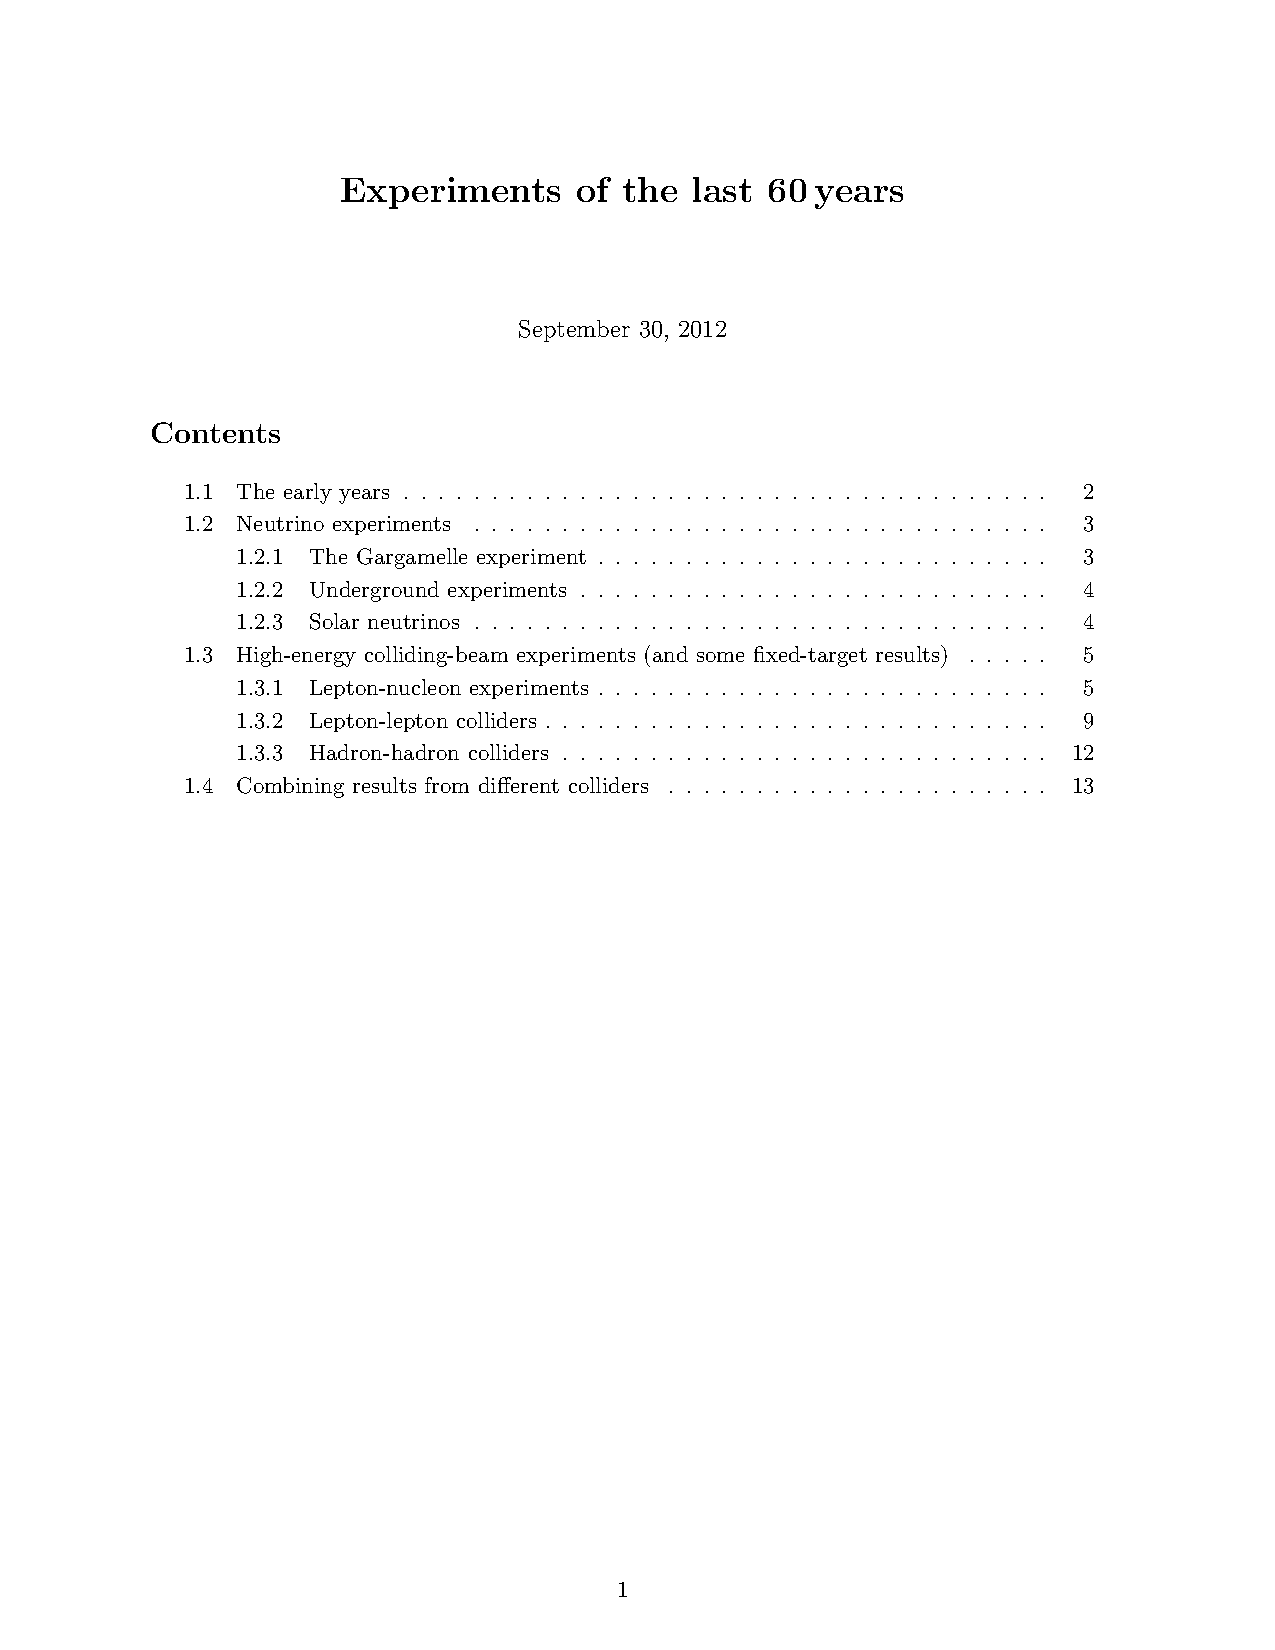
\includepdf[pages=-]{include/ExperimentalHighlights}

  \chapter{Special Relativity}
  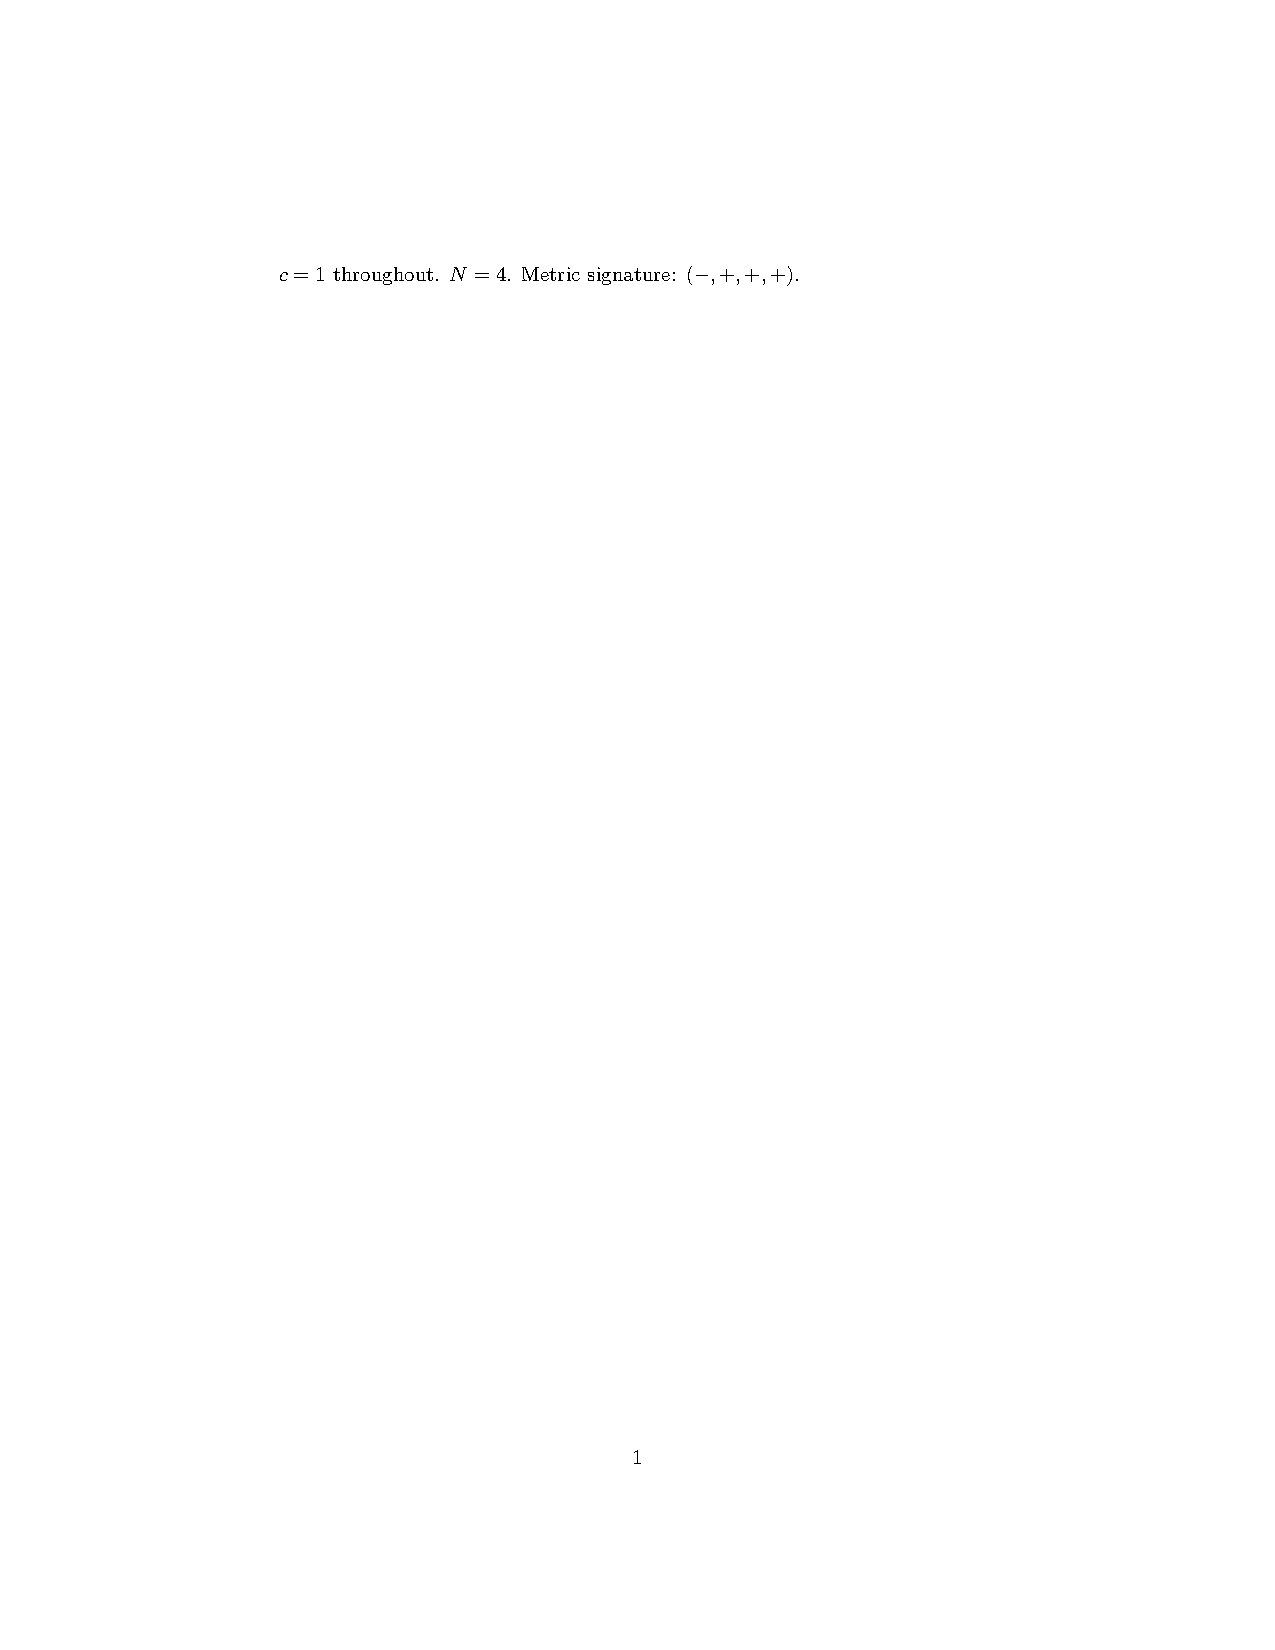
\includepdf[pages=-]{include/SR}

  \chapter{Fermi $beta$-Decay}
  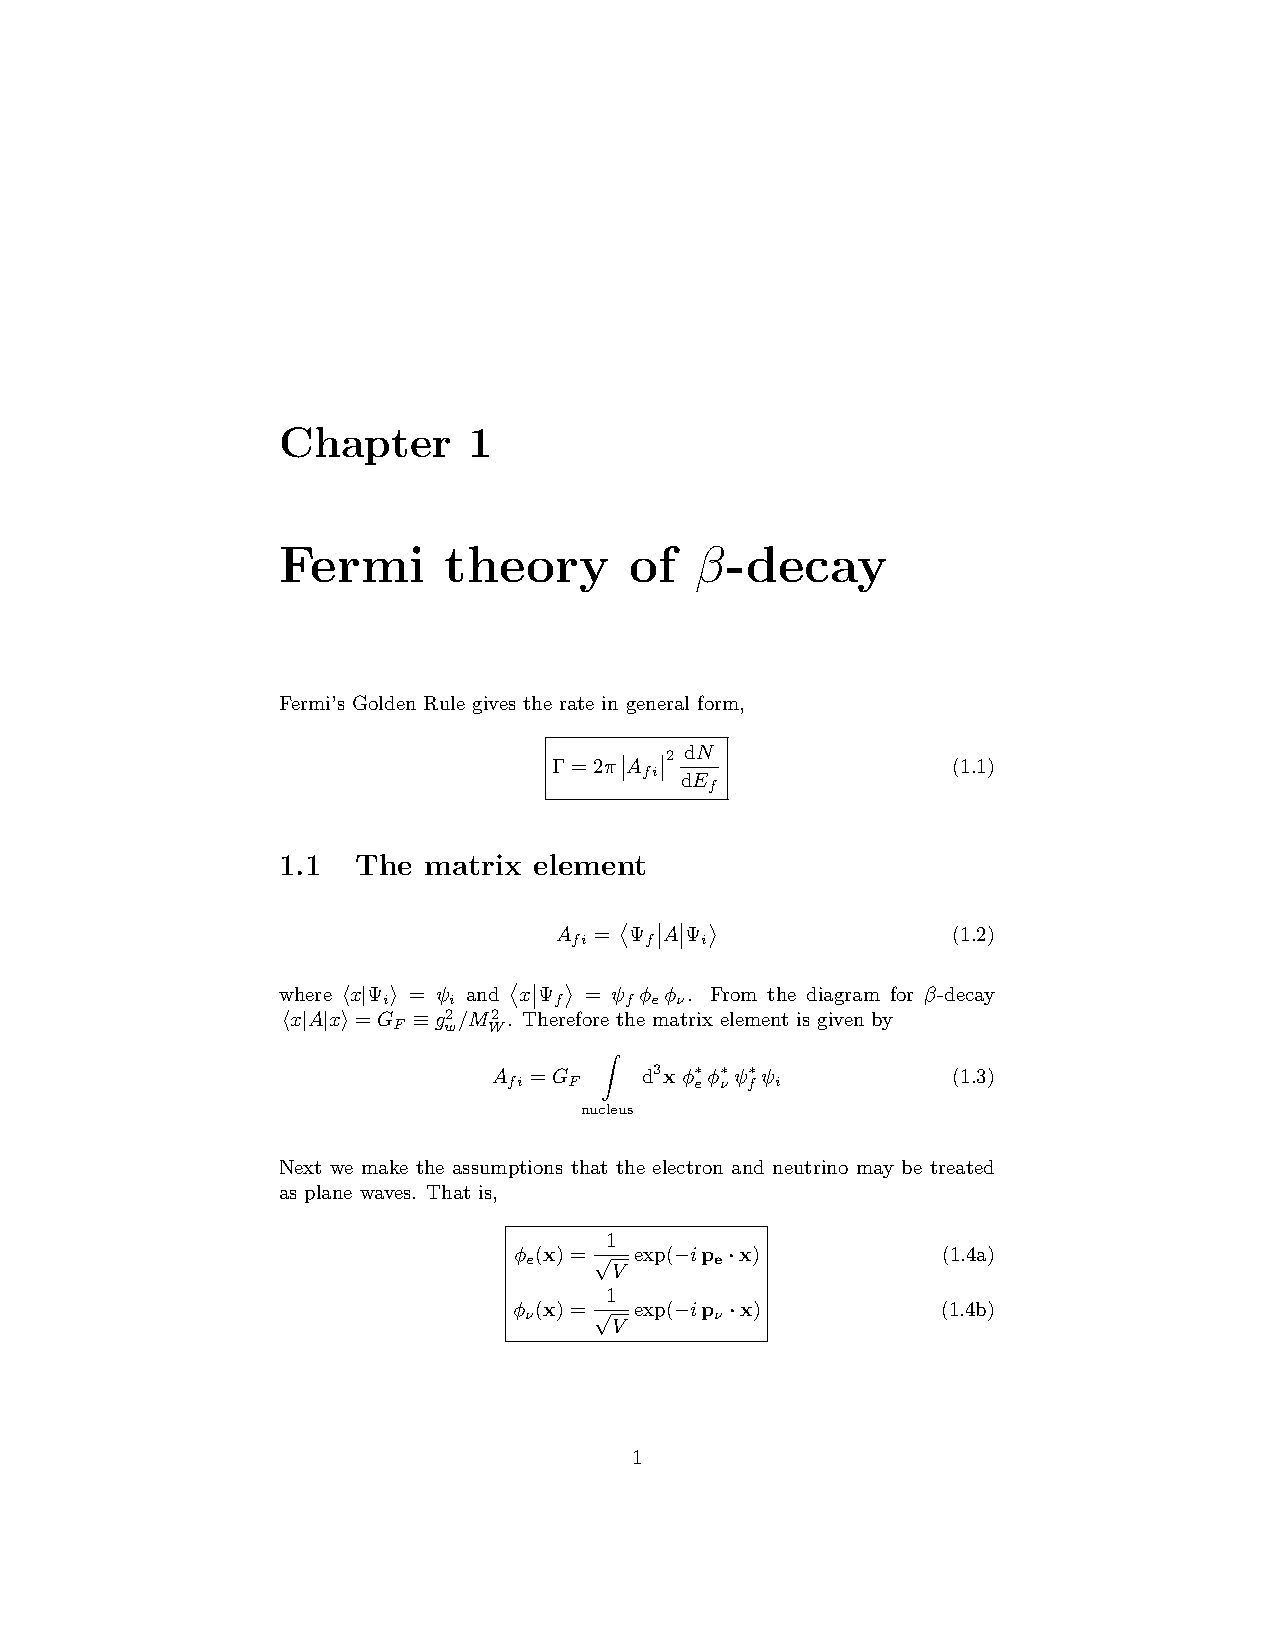
\includepdf[pages=-]{include/Subatomic}

  \chapter{2-Flavor Neutrino Model}
  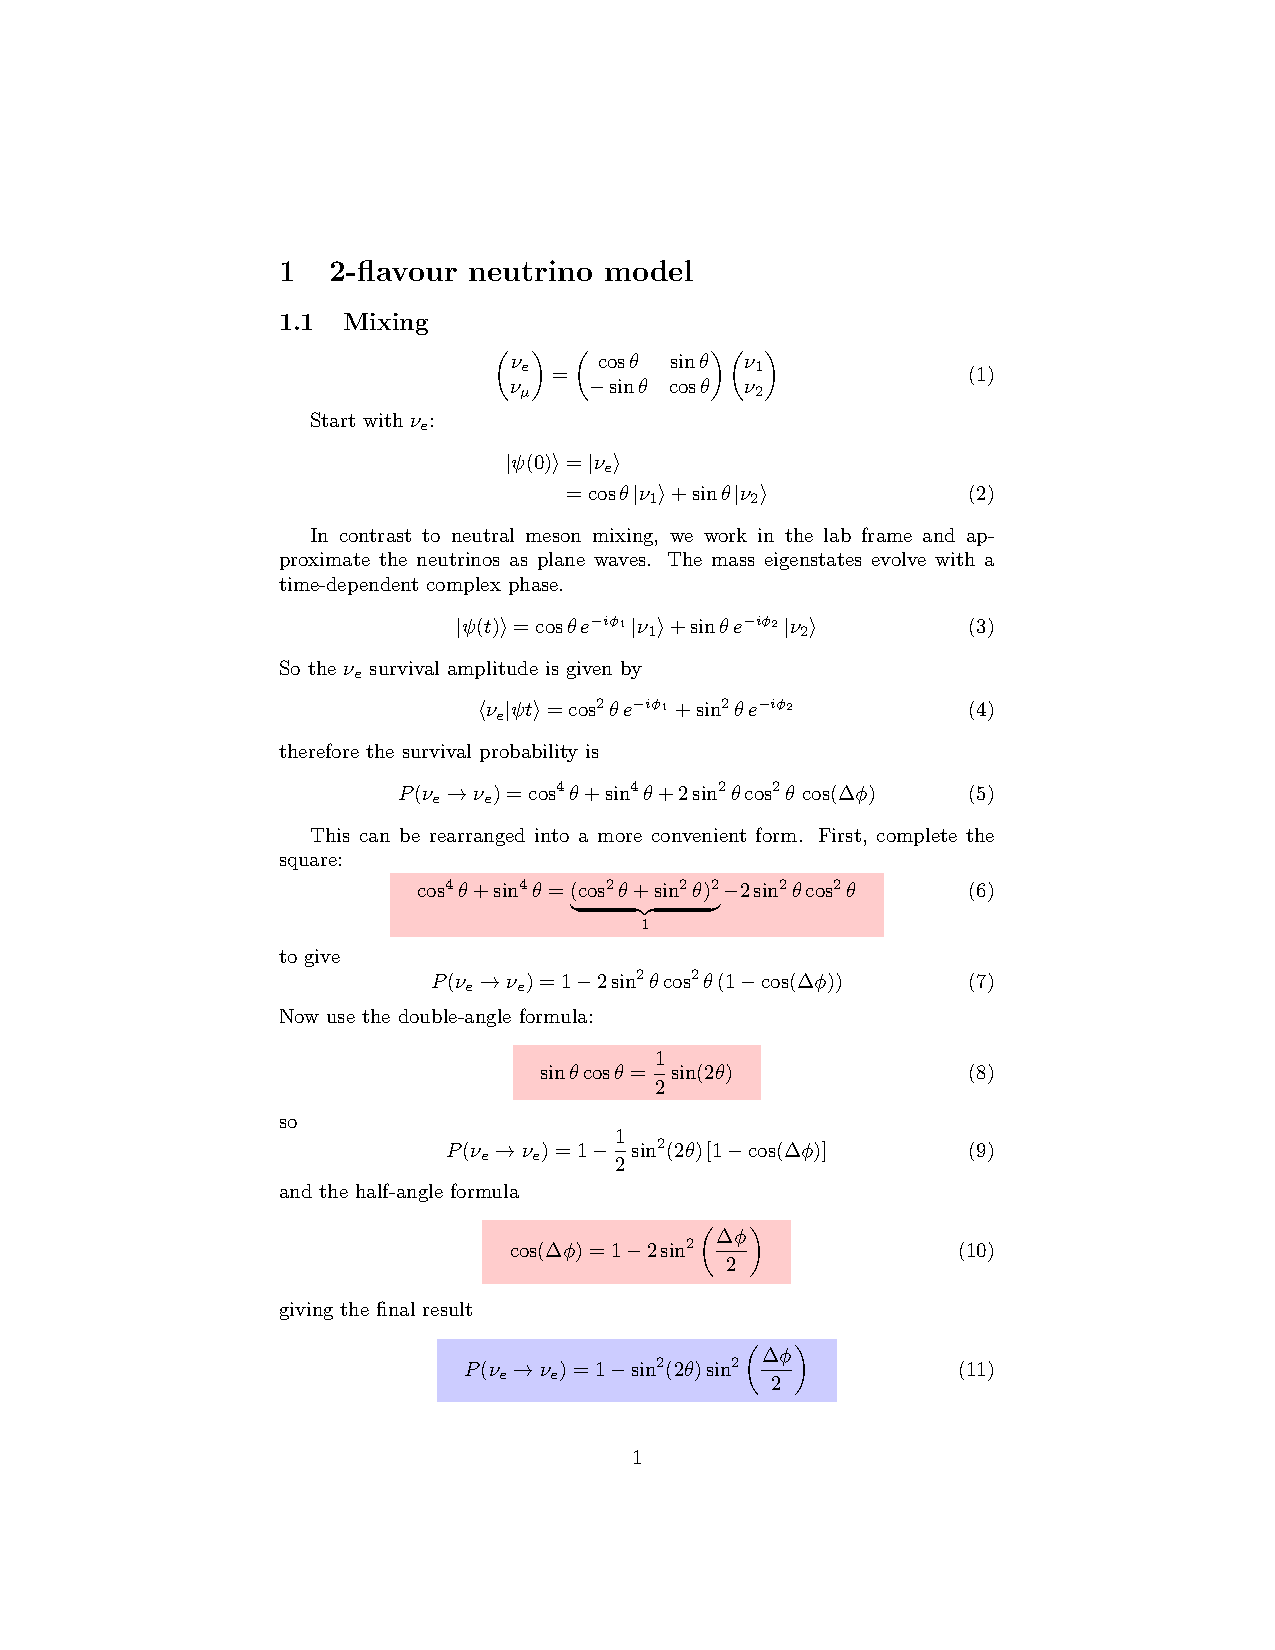
\includepdf[pages=-]{include/Neutrinos}

  \chapter{Electroweak Unification}
  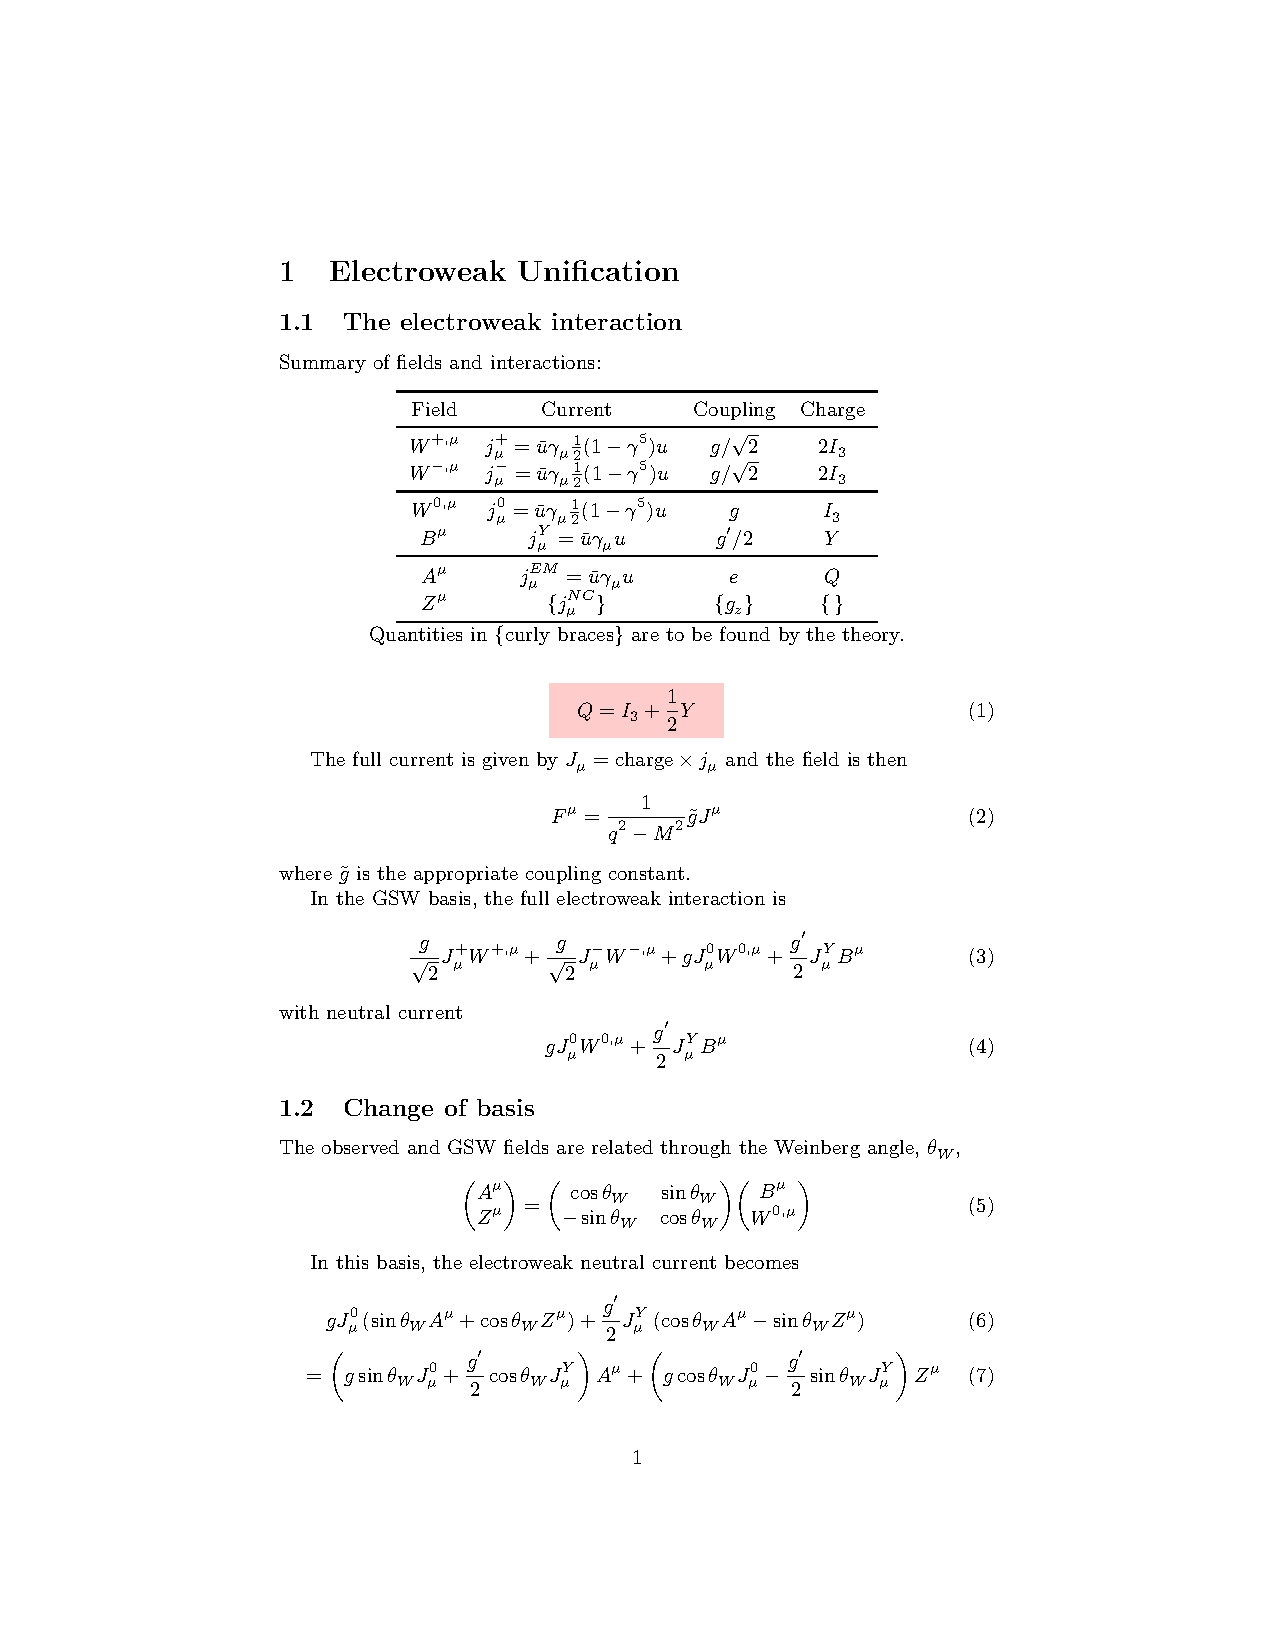
\includepdf[pages=-]{include/EW_Unification}

  \chapter{Lorentz Invariant Phase Space}
  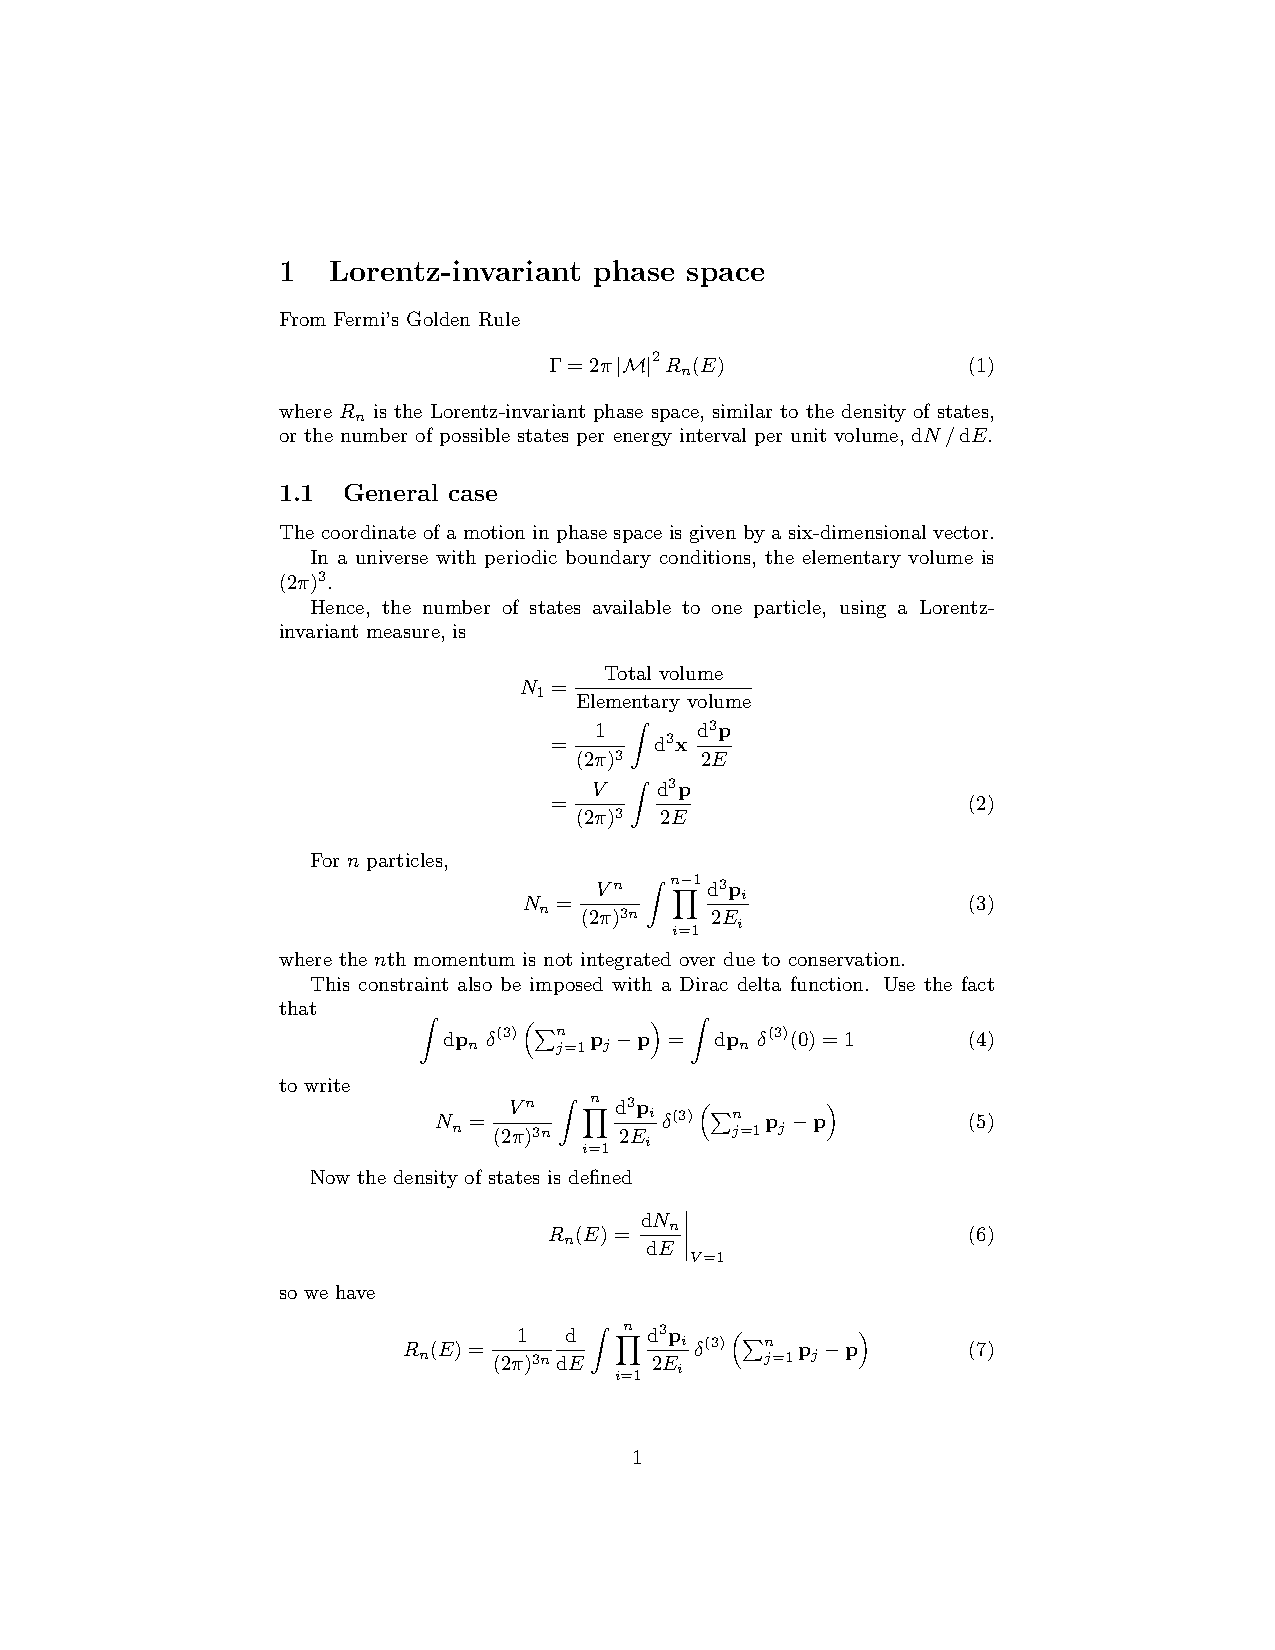
\includepdf[pages=-]{include/Phase_space}

\end{document}
